\INEchaptercarta{Alumnos en el ciclo básico}{}



\cajita{Inscritos en básicos }{El número de  inscritos en básicos se obtiene a partir del total de los alumnos registrados al treinta de marzo de cada año escolar, sin distinción de la edad y que se matriculan en el ciclo básico.
	
	 En el año 2009 se inscribieron 671,872 alumnos y en el 2014 se inscribieron 769,163, lo cual muestra un crecimiento de 14.5\%.}{Número de inscritos en el ciclo de educación básica}{República de Guatemala, serie histórica, en datos absolutos}{\ \\[0mm]\begin{tikzpicture}[x=1pt,y=1pt]  % Created by tikzDevice version 0.7.0 on 2015-08-28 13:08:39
% !TEX encoding = UTF-8 Unicode
\definecolor[named]{fillColor}{rgb}{1.00,1.00,1.00}
\path[use as bounding box,fill=fillColor,fill opacity=0.00] (0,0) rectangle (289.08,198.74);
\begin{scope}
\path[clip] (  0.00,  0.00) rectangle (289.08,198.74);
\definecolor[named]{drawColor}{rgb}{1.00,1.00,1.00}

\path[draw=drawColor,line width= 0.6pt,line join=round,line cap=round] (  0.00,  0.00) rectangle (289.08,198.74);
\end{scope}
\begin{scope}
\path[clip] (  0.00,  0.00) rectangle (289.08,198.74);

\path[] ( 14.70, 17.78) rectangle (280.54,191.48);

\path[] ( 14.70, 46.32) --
	(280.54, 46.32);

\path[] ( 14.70, 87.64) --
	(280.54, 87.64);

\path[] ( 14.70,128.96) --
	(280.54,128.96);

\path[] ( 14.70,170.28) --
	(280.54,170.28);

\path[] ( 14.70, 25.66) --
	(280.54, 25.66);

\path[] ( 14.70, 66.98) --
	(280.54, 66.98);

\path[] ( 14.70,108.30) --
	(280.54,108.30);

\path[] ( 14.70,149.62) --
	(280.54,149.62);

\path[] ( 14.70,190.94) --
	(280.54,190.94);

\path[] ( 45.37, 17.78) --
	( 45.37,191.48);

\path[] ( 96.50, 17.78) --
	( 96.50,191.48);

\path[] (147.62, 17.78) --
	(147.62,191.48);

\path[] (198.74, 17.78) --
	(198.74,191.48);

\path[] (249.87, 17.78) --
	(249.87,191.48);
\definecolor[named]{drawColor}{rgb}{0.00,0.00,1.00}

\path[draw=drawColor,line width= 1.7pt,line join=round] ( 45.37,164.47) --
	( 96.50,176.67) --
	(147.62,178.72) --
	(198.74,179.89) --
	(249.87,183.59);
\definecolor[named]{drawColor}{rgb}{0.00,0.00,0.00}

\node[text=drawColor,anchor=base,inner sep=0pt, outer sep=0pt, scale=  1.01] at ( 45.37,152.60) {671,872};

\node[text=drawColor,anchor=base east,inner sep=0pt, outer sep=0pt, scale=  1.01] at ( 90.72,176.67) {730,929};

\node[text=drawColor,anchor=base east,inner sep=0pt, outer sep=0pt, scale=  1.01] at (141.84,183.72) {740,877};

\node[text=drawColor,anchor=base east,inner sep=0pt, outer sep=0pt, scale=  1.01] at (192.97,183.89) {746,516};

\node[text=drawColor,anchor=base,inner sep=0pt, outer sep=0pt, scale=  1.01] at (249.87,187.54) {764,415};
\definecolor[named]{fillColor}{rgb}{0.00,0.00,0.00}

\path[draw=drawColor,line width= 0.1pt,line join=round,fill=fillColor] ( 14.70, 25.67) -- (280.54, 25.67);
\end{scope}
\begin{scope}
\path[clip] (  0.00,  0.00) rectangle (289.08,198.74);

\path[] ( 14.70, 17.78) --
	( 14.70,191.48);
\end{scope}
\begin{scope}
\path[clip] (  0.00,  0.00) rectangle (289.08,198.74);
\definecolor[named]{drawColor}{rgb}{1.00,1.00,1.00}

\node[text=drawColor,text opacity=0.00,anchor=base east,inner sep=0pt, outer sep=0pt, scale=  1.00] at (  7.58, 21.75) {0e+00};

\node[text=drawColor,text opacity=0.00,anchor=base east,inner sep=0pt, outer sep=0pt, scale=  1.00] at (  7.58, 63.07) {2e+05};

\node[text=drawColor,text opacity=0.00,anchor=base east,inner sep=0pt, outer sep=0pt, scale=  1.00] at (  7.58,104.39) {4e+05};

\node[text=drawColor,text opacity=0.00,anchor=base east,inner sep=0pt, outer sep=0pt, scale=  1.00] at (  7.58,145.71) {6e+05};

\node[text=drawColor,text opacity=0.00,anchor=base east,inner sep=0pt, outer sep=0pt, scale=  1.00] at (  7.58,187.03) {8e+05};
\end{scope}
\begin{scope}
\path[clip] (  0.00,  0.00) rectangle (289.08,198.74);

\path[] ( 10.43, 25.66) --
	( 14.70, 25.66);

\path[] ( 10.43, 66.98) --
	( 14.70, 66.98);

\path[] ( 10.43,108.30) --
	( 14.70,108.30);

\path[] ( 10.43,149.62) --
	( 14.70,149.62);

\path[] ( 10.43,190.94) --
	( 14.70,190.94);
\end{scope}
\begin{scope}
\path[clip] (  0.00,  0.00) rectangle (289.08,198.74);

\path[] ( 14.70, 17.78) --
	(280.54, 17.78);
\end{scope}
\begin{scope}
\path[clip] (  0.00,  0.00) rectangle (289.08,198.74);

\path[] ( 45.37, 13.51) --
	( 45.37, 17.78);

\path[] ( 96.50, 13.51) --
	( 96.50, 17.78);

\path[] (147.62, 13.51) --
	(147.62, 17.78);

\path[] (198.74, 13.51) --
	(198.74, 17.78);

\path[] (249.87, 13.51) --
	(249.87, 17.78);
\end{scope}
\begin{scope}
\path[clip] (  0.00,  0.00) rectangle (289.08,198.74);
\definecolor[named]{drawColor}{rgb}{0.00,0.00,0.00}

\node[text=drawColor,anchor=base,inner sep=0pt, outer sep=0pt, scale=  1.00] at ( 45.37,  2.85) {2009};

\node[text=drawColor,anchor=base,inner sep=0pt, outer sep=0pt, scale=  1.00] at ( 96.50,  2.85) {2010};

\node[text=drawColor,anchor=base,inner sep=0pt, outer sep=0pt, scale=  1.00] at (147.62,  2.85) {2011};

\node[text=drawColor,anchor=base,inner sep=0pt, outer sep=0pt, scale=  1.00] at (198.74,  2.85) {2012};

\node[text=drawColor,anchor=base,inner sep=0pt, outer sep=0pt, scale=  1.00] at (249.87,  2.85) {2014};
\end{scope}
  \end{tikzpicture}}{Instituto Nacional de Estadística, con datos del Ministerio de Educación}

\cajita{Inscritos en básicos por sexo}{La distribución por sexo de los alumnos inscritos en educación básica muestra que el 53.4\% fueron hombres y de mujeres  46.6\%.}{Distribución de inscritos en el ciclo de educación básica, por sexo}{República de Guatemala, año 2014, en porcentaje}{\ \\[0mm]\begin{tikzpicture}[x=1pt,y=1pt]  % Created by tikzDevice version 0.7.0 on 2015-08-28 13:08:47
% !TEX encoding = UTF-8 Unicode
\definecolor[named]{fillColor}{rgb}{1.00,1.00,1.00}
\path[use as bounding box,fill=fillColor,fill opacity=0.00] (0,0) rectangle (289.08,198.74);
\begin{scope}
\path[clip] ( 30.54,  0.00) rectangle (258.54,198.74);
\definecolor[named]{drawColor}{rgb}{1.00,1.00,1.00}

\path[draw=drawColor,line width= 0.6pt,line join=round,line cap=round] ( 30.54,  0.00) rectangle (258.54,198.74);
\end{scope}
\begin{scope}
\path[clip] (  0.00,  0.00) rectangle (289.08,198.74);

\path[] (  9.28,  7.11) rectangle (200.91,198.74);

\path[] (105.09,102.93) --
	(190.76, 93.06);

\path[] (105.09,102.93) --
	( 19.42,112.80);

\path[] (105.09,102.93) --
	(114.96,188.59);

\path[] (105.09,102.93) --
	(190.76, 93.06);

\path[] (105.09,102.93) --
	( 95.22, 17.26);

\path[] (105.09,102.93) --
	( 19.42,112.80);

\path[] (105.09,102.93) --
	(105.09,102.93) --
	(105.09,102.93) --
	(105.09,102.93) --
	(105.09,102.93) --
	(105.09,102.93) --
	(105.09,102.93) --
	(105.09,102.93) --
	(105.09,102.93) --
	(105.09,102.93) --
	(105.09,102.93) --
	(105.09,102.93) --
	(105.09,102.93) --
	(105.09,102.93) --
	(105.09,102.93) --
	(105.09,102.93) --
	(105.09,102.93) --
	(105.09,102.93) --
	(105.09,102.93) --
	(105.09,102.93) --
	(105.09,102.93) --
	(105.09,102.93) --
	(105.09,102.93) --
	(105.09,102.93) --
	(105.09,102.93) --
	(105.09,102.93) --
	(105.09,102.93) --
	(105.09,102.93) --
	(105.09,102.93) --
	(105.09,102.93) --
	(105.09,102.93) --
	(105.09,102.93) --
	(105.09,102.93) --
	(105.09,102.93) --
	(105.09,102.93) --
	(105.09,102.93) --
	(105.09,102.93) --
	(105.09,102.93) --
	(105.09,102.93) --
	(105.09,102.93) --
	(105.09,102.93) --
	(105.09,102.93) --
	(105.09,102.93) --
	(105.09,102.93) --
	(105.09,102.93) --
	(105.09,102.93) --
	(105.09,102.93) --
	(105.09,102.93) --
	(105.09,102.93) --
	(105.09,102.93) --
	(105.09,102.93) --
	(105.09,102.93) --
	(105.09,102.93) --
	(105.09,102.93) --
	(105.09,102.93) --
	(105.09,102.93) --
	(105.09,102.93) --
	(105.09,102.93) --
	(105.09,102.93) --
	(105.09,102.93) --
	(105.09,102.93) --
	(105.09,102.93) --
	(105.09,102.93) --
	(105.09,102.93) --
	(105.09,102.93) --
	(105.09,102.93) --
	(105.09,102.93) --
	(105.09,102.93) --
	(105.09,102.93) --
	(105.09,102.93) --
	(105.09,102.93) --
	(105.09,102.93) --
	(105.09,102.93) --
	(105.09,102.93) --
	(105.09,102.93) --
	(105.09,102.93) --
	(105.09,102.93) --
	(105.09,102.93) --
	(105.09,102.93) --
	(105.09,102.93) --
	(105.09,102.93) --
	(105.09,102.93) --
	(105.09,102.93) --
	(105.09,102.93) --
	(105.09,102.93) --
	(105.09,102.93) --
	(105.09,102.93) --
	(105.09,102.93) --
	(105.09,102.93) --
	(105.09,102.93) --
	(105.09,102.93) --
	(105.09,102.93) --
	(105.09,102.93) --
	(105.09,102.93) --
	(105.09,102.93) --
	(105.09,102.93) --
	(105.09,102.93) --
	(105.09,102.93) --
	(105.09,102.93) --
	(105.09,102.93);

\path[] (105.09,122.09) --
	(106.31,122.05) --
	(107.52,121.94) --
	(108.72,121.74) --
	(109.90,121.48) --
	(111.07,121.13) --
	(112.21,120.72) --
	(113.33,120.23) --
	(114.41,119.67) --
	(115.45,119.05) --
	(116.45,118.36) --
	(117.41,117.61) --
	(118.32,116.80) --
	(119.17,115.93) --
	(119.96,115.01) --
	(120.70,114.04) --
	(121.37,113.03) --
	(121.98,111.98) --
	(122.52,110.89) --
	(122.99,109.77) --
	(123.39,108.62) --
	(123.71,107.45) --
	(123.96,106.26) --
	(124.14,105.05) --
	(124.23,103.84) --
	(124.25,102.62) --
	(124.19,101.41) --
	(124.06,100.20) --
	(123.85, 99.00) --
	(123.56, 97.82) --
	(123.20, 96.66) --
	(122.77, 95.52) --
	(122.26, 94.42) --
	(121.69, 93.35) --
	(121.05, 92.31) --
	(120.34, 91.32) --
	(119.57, 90.38) --
	(118.75, 89.49) --
	(117.87, 88.65) --
	(116.94, 87.86) --
	(115.96, 87.14) --
	(114.93, 86.49) --
	(113.87, 85.90) --
	(112.77, 85.37) --
	(111.65, 84.92) --
	(110.49, 84.54) --
	(109.31, 84.24) --
	(108.12, 84.01) --
	(106.91, 83.85) --
	(105.70, 83.77) --
	(104.48, 83.77) --
	(103.27, 83.85) --
	(102.06, 84.01) --
	(100.87, 84.24) --
	( 99.69, 84.54) --
	( 98.54, 84.92) --
	( 97.41, 85.37) --
	( 96.31, 85.90) --
	( 95.25, 86.49) --
	( 94.22, 87.14) --
	( 93.25, 87.86) --
	( 92.31, 88.65) --
	( 91.43, 89.49) --
	( 90.61, 90.38) --
	( 89.84, 91.32) --
	( 89.14, 92.31) --
	( 88.50, 93.35) --
	( 87.92, 94.42) --
	( 87.42, 95.52) --
	( 86.98, 96.66) --
	( 86.62, 97.82) --
	( 86.33, 99.00) --
	( 86.12,100.20) --
	( 85.99,101.41) --
	( 85.93,102.62) --
	( 85.95,103.84) --
	( 86.05,105.05) --
	( 86.22,106.26) --
	( 86.47,107.45) --
	( 86.79,108.62) --
	( 87.19,109.77) --
	( 87.66,110.89) --
	( 88.20,111.98) --
	( 88.81,113.03) --
	( 89.48,114.04) --
	( 90.22,115.01) --
	( 91.01,115.93) --
	( 91.87,116.80) --
	( 92.77,117.61) --
	( 93.73,118.36) --
	( 94.73,119.05) --
	( 95.77,119.67) --
	( 96.85,120.23) --
	( 97.97,120.72) --
	( 99.11,121.13) --
	(100.28,121.48) --
	(101.46,121.74) --
	(102.67,121.94) --
	(103.88,122.05) --
	(105.09,122.09);

\path[] (105.09,141.25) --
	(107.52,141.18) --
	(109.94,140.95) --
	(112.34,140.56) --
	(114.72,140.03) --
	(117.05,139.34) --
	(119.34,138.51) --
	(121.56,137.53) --
	(123.72,136.42) --
	(125.81,135.17) --
	(127.81,133.79) --
	(129.73,132.29) --
	(131.54,130.67) --
	(133.24,128.93) --
	(134.84,127.09) --
	(136.31,125.16) --
	(137.66,123.13) --
	(138.87,121.03) --
	(139.95,118.85) --
	(140.89,116.61) --
	(141.69,114.31) --
	(142.34,111.96) --
	(142.83,109.58) --
	(143.18,107.18) --
	(143.37,104.75) --
	(143.41,102.32) --
	(143.30, 99.89) --
	(143.03, 97.47) --
	(142.60, 95.08) --
	(142.03, 92.72) --
	(141.31, 90.39) --
	(140.44, 88.12) --
	(139.43, 85.91) --
	(138.28, 83.76) --
	(137.00, 81.70) --
	(135.59, 79.72) --
	(134.06, 77.83) --
	(132.41, 76.04) --
	(130.65, 74.36) --
	(128.78, 72.80) --
	(126.82, 71.36) --
	(124.78, 70.04) --
	(122.65, 68.86) --
	(120.46, 67.82) --
	(118.20, 66.91) --
	(115.89, 66.15) --
	(113.53, 65.54) --
	(111.15, 65.08) --
	(108.73, 64.78) --
	(106.31, 64.62) --
	(103.88, 64.62) --
	(101.45, 64.78) --
	( 99.04, 65.08) --
	( 96.65, 65.54) --
	( 94.29, 66.15) --
	( 91.98, 66.91) --
	( 89.73, 67.82) --
	( 87.53, 68.86) --
	( 85.40, 70.04) --
	( 83.36, 71.36) --
	( 81.40, 72.80) --
	( 79.54, 74.36) --
	( 77.78, 76.04) --
	( 76.13, 77.83) --
	( 74.59, 79.72) --
	( 73.18, 81.70) --
	( 71.90, 83.76) --
	( 70.75, 85.91) --
	( 69.74, 88.12) --
	( 68.87, 90.39) --
	( 68.15, 92.72) --
	( 67.58, 95.08) --
	( 67.16, 97.47) --
	( 66.89, 99.89) --
	( 66.77,102.32) --
	( 66.81,104.75) --
	( 67.00,107.18) --
	( 67.35,109.58) --
	( 67.85,111.96) --
	( 68.49,114.31) --
	( 69.29,116.61) --
	( 70.23,118.85) --
	( 71.31,121.03) --
	( 72.52,123.13) --
	( 73.87,125.16) --
	( 75.34,127.09) --
	( 76.94,128.93) --
	( 78.64,130.67) --
	( 80.46,132.29) --
	( 82.37,133.79) --
	( 84.37,135.17) --
	( 86.46,136.42) --
	( 88.62,137.53) --
	( 90.85,138.51) --
	( 93.13,139.34) --
	( 95.47,140.03) --
	( 97.84,140.56) --
	(100.24,140.95) --
	(102.66,141.18) --
	(105.09,141.25);

\path[] (105.09,160.42) --
	(108.74,160.30) --
	(112.37,159.95) --
	(115.97,159.38) --
	(119.53,158.57) --
	(123.03,157.55) --
	(126.46,156.30) --
	(129.80,154.84) --
	(133.04,153.16) --
	(136.17,151.29) --
	(139.18,149.22) --
	(142.04,146.97) --
	(144.76,144.53) --
	(147.32,141.93) --
	(149.71,139.18) --
	(151.92,136.27) --
	(153.94,133.24) --
	(155.76,130.08) --
	(157.38,126.81) --
	(158.79,123.44) --
	(159.99,120.00) --
	(160.96,116.48) --
	(161.71,112.91) --
	(162.23,109.30) --
	(162.51,105.66) --
	(162.57,102.02) --
	(162.40, 98.37) --
	(161.99, 94.75) --
	(161.36, 91.15) --
	(160.50, 87.61) --
	(159.42, 84.13) --
	(158.12, 80.72) --
	(156.60, 77.40) --
	(154.88, 74.18) --
	(152.95, 71.08) --
	(150.84, 68.11) --
	(148.54, 65.28) --
	(146.06, 62.60) --
	(143.42, 60.08) --
	(140.63, 57.74) --
	(137.69, 55.58) --
	(134.62, 53.60) --
	(131.43, 51.83) --
	(128.14, 50.26) --
	(124.75, 48.91) --
	(121.29, 47.77) --
	(117.76, 46.85) --
	(114.17, 46.16) --
	(110.56, 45.70) --
	(106.92, 45.47) --
	(103.27, 45.47) --
	( 99.63, 45.70) --
	( 96.01, 46.16) --
	( 92.43, 46.85) --
	( 88.89, 47.77) --
	( 85.43, 48.91) --
	( 82.04, 50.26) --
	( 78.75, 51.83) --
	( 75.56, 53.60) --
	( 72.49, 55.58) --
	( 69.55, 57.74) --
	( 66.76, 60.08) --
	( 64.12, 62.60) --
	( 61.64, 65.28) --
	( 59.34, 68.11) --
	( 57.23, 71.08) --
	( 55.30, 74.18) --
	( 53.58, 77.40) --
	( 52.07, 80.72) --
	( 50.76, 84.13) --
	( 49.68, 87.61) --
	( 48.82, 91.15) --
	( 48.19, 94.75) --
	( 47.78, 98.37) --
	( 47.61,102.02) --
	( 47.67,105.66) --
	( 47.96,109.30) --
	( 48.48,112.91) --
	( 49.22,116.48) --
	( 50.19,120.00) --
	( 51.39,123.44) --
	( 52.80,126.81) --
	( 54.42,130.08) --
	( 56.24,133.24) --
	( 58.26,136.27) --
	( 60.47,139.18) --
	( 62.86,141.93) --
	( 65.42,144.53) --
	( 68.14,146.97) --
	( 71.01,149.22) --
	( 74.01,151.29) --
	( 77.14,153.16) --
	( 80.38,154.84) --
	( 83.72,156.30) --
	( 87.15,157.55) --
	( 90.65,158.57) --
	( 94.21,159.38) --
	( 97.81,159.95) --
	(101.44,160.30) --
	(105.09,160.42);

\path[] (105.09,179.58) --
	(109.95,179.43) --
	(114.79,178.96) --
	(119.60,178.19) --
	(124.34,177.12) --
	(129.01,175.75) --
	(133.58,174.09) --
	(138.04,172.14) --
	(142.36,169.91) --
	(146.53,167.41) --
	(150.54,164.65) --
	(154.36,161.65) --
	(157.99,158.40) --
	(161.40,154.94) --
	(164.58,151.26) --
	(167.53,147.39) --
	(170.22,143.34) --
	(172.66,139.13) --
	(174.82,134.77) --
	(176.70,130.28) --
	(178.29,125.69) --
	(179.58,121.00) --
	(180.58,116.24) --
	(181.27,111.42) --
	(181.66,106.58) --
	(181.73,101.71) --
	(181.50, 96.85) --
	(180.96, 92.02) --
	(180.12, 87.23) --
	(178.97, 82.50) --
	(177.53, 77.86) --
	(175.79, 73.31) --
	(173.77, 68.89) --
	(171.47, 64.60) --
	(168.91, 60.47) --
	(166.09, 56.51) --
	(163.02, 52.73) --
	(159.72, 49.16) --
	(156.20, 45.80) --
	(152.47, 42.68) --
	(148.56, 39.79) --
	(144.47, 37.16) --
	(140.21, 34.80) --
	(135.82, 32.71) --
	(131.31, 30.90) --
	(126.69, 29.38) --
	(121.98, 28.16) --
	(117.20, 27.24) --
	(112.38, 26.62) --
	(107.52, 26.31) --
	(102.66, 26.31) --
	( 97.80, 26.62) --
	( 92.98, 27.24) --
	( 88.20, 28.16) --
	( 83.50, 29.38) --
	( 78.87, 30.90) --
	( 74.36, 32.71) --
	( 69.97, 34.80) --
	( 65.72, 37.16) --
	( 61.62, 39.79) --
	( 57.71, 42.68) --
	( 53.98, 45.80) --
	( 50.46, 49.16) --
	( 47.16, 52.73) --
	( 44.09, 56.51) --
	( 41.27, 60.47) --
	( 38.71, 64.60) --
	( 36.41, 68.89) --
	( 34.39, 73.31) --
	( 32.66, 77.86) --
	( 31.21, 82.50) --
	( 30.06, 87.23) --
	( 29.22, 92.02) --
	( 28.68, 96.85) --
	( 28.45,101.71) --
	( 28.53,106.58) --
	( 28.91,111.42) --
	( 29.60,116.24) --
	( 30.60,121.00) --
	( 31.90,125.69) --
	( 33.49,130.28) --
	( 35.37,134.77) --
	( 37.53,139.13) --
	( 39.96,143.34) --
	( 42.65,147.39) --
	( 45.60,151.26) --
	( 48.78,154.94) --
	( 52.20,158.40) --
	( 55.82,161.65) --
	( 59.64,164.65) --
	( 63.65,167.41) --
	( 67.82,169.91) --
	( 72.15,172.14) --
	( 76.60,174.09) --
	( 81.17,175.75) --
	( 85.84,177.12) --
	( 90.58,178.19) --
	( 95.39,178.96) --
	(100.23,179.43) --
	(105.09,179.58);

\path[] (105.09,189.16) --
	(110.56,188.99) --
	(116.01,188.47) --
	(121.41,187.60) --
	(126.75,186.40) --
	(132.00,184.86) --
	(137.14,182.98) --
	(142.15,180.79) --
	(147.02,178.28) --
	(151.71,175.47) --
	(156.22,172.37) --
	(160.52,168.99) --
	(164.60,165.34) --
	(168.44,161.44) --
	(172.02,157.30) --
	(175.33,152.95) --
	(178.37,148.39) --
	(181.10,143.65) --
	(183.53,138.75) --
	(185.65,133.70) --
	(187.44,128.53) --
	(188.89,123.26) --
	(190.01,117.90) --
	(190.79,112.49) --
	(191.23,107.03) --
	(191.31,101.56) --
	(191.05, 96.09) --
	(190.45, 90.66) --
	(189.50, 85.27) --
	(188.21, 79.95) --
	(186.58, 74.72) --
	(184.63, 69.61) --
	(182.36, 64.63) --
	(179.77, 59.81) --
	(176.89, 55.16) --
	(173.71, 50.70) --
	(170.26, 46.46) --
	(166.55, 42.44) --
	(162.59, 38.66) --
	(158.40, 35.14) --
	(153.99, 31.90) --
	(149.39, 28.94) --
	(144.61, 26.28) --
	(139.66, 23.93) --
	(134.58, 21.90) --
	(129.39, 20.19) --
	(124.09, 18.81) --
	(118.72, 17.78) --
	(113.29, 17.09) --
	(107.83, 16.74) --
	(102.36, 16.74) --
	( 96.89, 17.09) --
	( 91.47, 17.78) --
	( 86.09, 18.81) --
	( 80.80, 20.19) --
	( 75.60, 21.90) --
	( 70.52, 23.93) --
	( 65.58, 26.28) --
	( 60.80, 28.94) --
	( 56.19, 31.90) --
	( 51.79, 35.14) --
	( 47.59, 38.66) --
	( 43.63, 42.44) --
	( 39.92, 46.46) --
	( 36.47, 50.70) --
	( 33.30, 55.16) --
	( 30.41, 59.81) --
	( 27.83, 64.63) --
	( 25.55, 69.61) --
	( 23.60, 74.72) --
	( 21.98, 79.95) --
	( 20.69, 85.27) --
	( 19.74, 90.66) --
	( 19.13, 96.09) --
	( 18.87,101.56) --
	( 18.96,107.03) --
	( 19.39,112.49) --
	( 20.17,117.90) --
	( 21.29,123.26) --
	( 22.75,128.53) --
	( 24.54,133.70) --
	( 26.65,138.75) --
	( 29.08,143.65) --
	( 31.82,148.39) --
	( 34.85,152.95) --
	( 38.16,157.30) --
	( 41.74,161.44) --
	( 45.58,165.34) --
	( 49.66,168.99) --
	( 53.96,172.37) --
	( 58.47,175.47) --
	( 63.16,178.28) --
	( 68.03,180.79) --
	( 73.04,182.98) --
	( 78.18,184.86) --
	( 83.43,186.40) --
	( 88.77,187.60) --
	( 94.17,188.47) --
	( 99.62,188.99) --
	(105.09,189.16);
\definecolor[named]{drawColor}{rgb}{1.00,1.00,1.00}
\definecolor[named]{fillColor}{rgb}{0.00,0.00,1.00}

\path[draw=drawColor,line width= 0.6pt,line join=round,line cap=round,fill=fillColor] ( 96.37, 65.61) --
	( 95.75, 62.94) --
	( 95.13, 60.27) --
	( 94.51, 57.61) --
	( 93.88, 54.94) --
	( 93.26, 52.28) --
	( 92.64, 49.61) --
	( 92.02, 46.95) --
	( 91.39, 44.28) --
	( 90.77, 41.61) --
	( 90.15, 38.95) --
	( 89.53, 36.28) --
	( 88.90, 33.62) --
	( 88.28, 30.95) --
	( 87.66, 28.28) --
	( 87.66, 28.28) --
	( 90.21, 27.73) --
	( 92.78, 27.27) --
	( 95.36, 26.90) --
	( 97.95, 26.61) --
	(100.56, 26.41) --
	(103.16, 26.30) --
	(105.77, 26.28) --
	(108.38, 26.35) --
	(110.99, 26.50) --
	(113.59, 26.75) --
	(116.18, 27.08) --
	(118.75, 27.50) --
	(121.31, 28.01) --
	(123.85, 28.61) --
	(126.37, 29.29) --
	(128.87, 30.06) --
	(131.33, 30.91) --
	(133.77, 31.84) --
	(136.17, 32.86) --
	(138.54, 33.96) --
	(140.87, 35.14) --
	(143.16, 36.40) --
	(145.40, 37.73) --
	(147.60, 39.14) --
	(149.74, 40.62) --
	(151.84, 42.18) --
	(153.88, 43.81) --
	(155.86, 45.50) --
	(157.79, 47.26) --
	(159.65, 49.09) --
	(161.45, 50.98) --
	(163.19, 52.93) --
	(164.86, 54.93) --
	(166.46, 57.00) --
	(167.99, 59.11) --
	(169.44, 61.28) --
	(170.82, 63.49) --
	(172.13, 65.76) --
	(173.35, 68.06) --
	(174.50, 70.40) --
	(175.57, 72.79) --
	(176.55, 75.20) --
	(177.46, 77.65) --
	(178.27, 80.13) --
	(179.01, 82.63) --
	(179.66, 85.16) --
	(180.22, 87.71) --
	(180.69, 90.28) --
	(181.08, 92.86) --
	(181.38, 95.45) --
	(181.59, 98.05) --
	(181.71,100.66) --
	(181.74,103.27) --
	(181.69,105.88) --
	(181.54,108.48) --
	(181.31,111.08) --
	(180.99,113.67) --
	(180.58,116.25) --
	(180.08,118.81) --
	(179.49,121.36) --
	(178.82,123.88) --
	(178.07,126.38) --
	(177.23,128.85) --
	(176.30,131.29) --
	(175.30,133.70) --
	(174.21,136.07) --
	(173.04,138.40) --
	(171.79,140.70) --
	(170.47,142.94) --
	(169.07,145.15) --
	(167.59,147.30) --
	(166.05,149.40) --
	(164.43,151.45) --
	(162.74,153.44) --
	(160.99,155.38) --
	(159.17,157.25) --
	(157.29,159.06) --
	(155.35,160.80) --
	(153.35,162.48) --
	(151.29,164.09) --
	(149.19,165.63) --
	(147.03,167.09) --
	(144.82,168.48) --
	(142.56,169.80) --
	(140.26,171.03) --
	(137.92,172.19) --
	(135.55,173.27) --
	(133.14,174.27) --
	(130.69,175.18) --
	(128.22,176.01) --
	(125.71,176.75) --
	(123.19,177.41) --
	(120.64,177.99) --
	(118.08,178.47) --
	(115.50,178.87) --
	(112.91,179.18) --
	(110.31,179.40) --
	(107.70,179.54) --
	(105.09,179.58) --
	(105.09,179.58) --
	(105.09,176.84) --
	(105.09,174.10) --
	(105.09,171.37) --
	(105.09,168.63) --
	(105.09,165.89) --
	(105.09,163.15) --
	(105.09,160.42) --
	(105.09,157.68) --
	(105.09,154.94) --
	(105.09,152.20) --
	(105.09,149.47) --
	(105.09,146.73) --
	(105.09,143.99) --
	(105.09,141.25) --
	(105.09,141.25) --
	(107.73,141.16) --
	(110.35,140.89) --
	(112.95,140.44) --
	(115.51,139.81) --
	(118.02,139.01) --
	(120.47,138.03) --
	(122.84,136.89) --
	(125.14,135.59) --
	(127.33,134.14) --
	(129.43,132.54) --
	(131.40,130.79) --
	(133.26,128.92) --
	(134.98,126.92) --
	(136.56,124.81) --
	(137.99,122.59) --
	(139.26,120.29) --
	(140.37,117.90) --
	(141.32,115.44) --
	(142.09,112.92) --
	(142.69,110.35) --
	(143.11,107.75) --
	(143.35,105.12) --
	(143.41,102.49) --
	(143.29, 99.85) --
	(142.99, 97.23) --
	(142.51, 94.64) --
	(141.85, 92.09) --
	(141.02, 89.59) --
	(140.02, 87.15) --
	(138.85, 84.79) --
	(137.52, 82.51) --
	(136.04, 80.33) --
	(134.42, 78.25) --
	(132.65, 76.29) --
	(130.76, 74.46) --
	(128.74, 72.77) --
	(126.61, 71.21) --
	(124.38, 69.81) --
	(122.05, 68.56) --
	(119.65, 67.48) --
	(117.18, 66.56) --
	(114.65, 65.81) --
	(112.08, 65.24) --
	(109.47, 64.85) --
	(106.84, 64.64) --
	(104.21, 64.61) --
	(101.58, 64.76) --
	( 98.96, 65.10) --
	( 96.37, 65.61) --
	cycle;
\definecolor[named]{fillColor}{rgb}{0.62,0.73,1.00}

\path[draw=drawColor,line width= 0.6pt,line join=round,line cap=round,fill=fillColor] (105.09,141.25) --
	(105.09,143.99) --
	(105.09,146.73) --
	(105.09,149.47) --
	(105.09,152.20) --
	(105.09,154.94) --
	(105.09,157.68) --
	(105.09,160.42) --
	(105.09,163.15) --
	(105.09,165.89) --
	(105.09,168.63) --
	(105.09,171.37) --
	(105.09,174.10) --
	(105.09,176.84) --
	(105.09,179.58) --
	(105.09,179.58) --
	(102.50,179.54) --
	( 99.90,179.40) --
	( 97.32,179.18) --
	( 94.74,178.88) --
	( 92.18,178.48) --
	( 89.62,178.00) --
	( 87.09,177.44) --
	( 84.58,176.78) --
	( 82.09,176.05) --
	( 79.63,175.23) --
	( 77.20,174.32) --
	( 74.79,173.34) --
	( 72.43,172.27) --
	( 70.10,171.13) --
	( 67.81,169.90) --
	( 65.56,168.60) --
	( 63.36,167.23) --
	( 61.21,165.78) --
	( 59.11,164.25) --
	( 57.06,162.66) --
	( 55.06,161.00) --
	( 53.13,159.28) --
	( 51.25,157.48) --
	( 49.43,155.63) --
	( 47.68,153.71) --
	( 45.99,151.74) --
	( 44.37,149.71) --
	( 42.82,147.63) --
	( 41.35,145.50) --
	( 39.94,143.31) --
	( 38.61,141.09) --
	( 37.36,138.81) --
	( 36.18,136.50) --
	( 35.09,134.15) --
	( 34.07,131.76) --
	( 33.13,129.34) --
	( 32.28,126.89) --
	( 31.51,124.41) --
	( 30.83,121.90) --
	( 30.23,119.38) --
	( 29.71,116.84) --
	( 29.28,114.28) --
	( 28.94,111.70) --
	( 28.69,109.12) --
	( 28.52,106.53) --
	( 28.45,103.93) --
	( 28.46,101.34) --
	( 28.55, 98.75) --
	( 28.74, 96.16) --
	( 29.01, 93.58) --
	( 29.37, 91.01) --
	( 29.82, 88.45) --
	( 30.35, 85.91) --
	( 30.97, 83.39) --
	( 31.68, 80.89) --
	( 32.46, 78.42) --
	( 33.34, 75.97) --
	( 34.29, 73.56) --
	( 35.32, 71.18) --
	( 36.44, 68.83) --
	( 37.63, 66.53) --
	( 38.90, 64.27) --
	( 40.25, 62.05) --
	( 41.67, 59.88) --
	( 43.17, 57.75) --
	( 44.73, 55.68) --
	( 46.36, 53.67) --
	( 48.07, 51.71) --
	( 49.83, 49.81) --
	( 51.66, 47.97) --
	( 53.55, 46.19) --
	( 55.50, 44.48) --
	( 57.51, 42.83) --
	( 59.57, 41.25) --
	( 61.69, 39.75) --
	( 63.85, 38.31) --
	( 66.06, 36.96) --
	( 68.32, 35.67) --
	( 70.62, 34.47) --
	( 72.95, 33.34) --
	( 75.33, 32.29) --
	( 77.74, 31.32) --
	( 80.18, 30.44) --
	( 82.65, 29.64) --
	( 85.14, 28.92) --
	( 87.66, 28.28) --
	( 87.66, 28.28) --
	( 88.28, 30.95) --
	( 88.90, 33.62) --
	( 89.53, 36.28) --
	( 90.15, 38.95) --
	( 90.77, 41.61) --
	( 91.39, 44.28) --
	( 92.02, 46.95) --
	( 92.64, 49.61) --
	( 93.26, 52.28) --
	( 93.88, 54.94) --
	( 94.51, 57.61) --
	( 95.13, 60.27) --
	( 95.75, 62.94) --
	( 96.37, 65.61) --
	( 96.37, 65.61) --
	( 93.87, 66.28) --
	( 91.41, 67.13) --
	( 89.02, 68.13) --
	( 86.71, 69.30) --
	( 84.47, 70.62) --
	( 82.33, 72.09) --
	( 80.30, 73.70) --
	( 78.38, 75.45) --
	( 76.58, 77.32) --
	( 74.91, 79.31) --
	( 73.38, 81.40) --
	( 72.00, 83.60) --
	( 70.76, 85.88) --
	( 69.69, 88.24) --
	( 68.78, 90.67) --
	( 68.03, 93.16) --
	( 67.46, 95.69) --
	( 67.05, 98.25) --
	( 66.82,100.84) --
	( 66.77,103.43) --
	( 66.89,106.02) --
	( 67.19,108.60) --
	( 67.66,111.15) --
	( 68.30,113.67) --
	( 69.11,116.13) --
	( 70.09,118.54) --
	( 71.22,120.87) --
	( 72.52,123.12) --
	( 73.96,125.28) --
	( 75.54,127.33) --
	( 77.26,129.28) --
	( 79.11,131.10) --
	( 81.07,132.80) --
	( 83.15,134.35) --
	( 85.33,135.76) --
	( 87.59,137.03) --
	( 89.94,138.13) --
	( 92.36,139.08) --
	( 94.84,139.86) --
	( 97.36,140.47) --
	( 99.92,140.90) --
	(102.50,141.17) --
	(105.09,141.25) --
	cycle;
\definecolor[named]{drawColor}{rgb}{0.00,0.00,0.00}

\node[text=drawColor,anchor=base,inner sep=0pt, outer sep=0pt, scale=  1.00] at (190.76, 89.15) {53.7};

\node[text=drawColor,anchor=base,inner sep=0pt, outer sep=0pt, scale=  1.00] at ( 19.42,108.89) {46.3};
\end{scope}
\begin{scope}
\path[clip] (  0.00,  0.00) rectangle (289.08,198.74);

\path[] (  9.28,  7.11) --
	(  9.28,198.74);
\end{scope}
\begin{scope}
\path[clip] (  0.00,  0.00) rectangle (289.08,198.74);

\path[] (  5.01,102.93) --
	(  9.28,102.93);

\path[] (  5.01,122.09) --
	(  9.28,122.09);

\path[] (  5.01,141.25) --
	(  9.28,141.25);

\path[] (  5.01,160.42) --
	(  9.28,160.42);

\path[] (  5.01,179.58) --
	(  9.28,179.58);
\end{scope}
\begin{scope}
\path[clip] (  0.00,  0.00) rectangle (289.08,198.74);

\path[] (  9.28,  7.11) --
	(200.91,  7.11);
\end{scope}
\coordinate (rect) at (192.72,99.37);
\coordinate (desY) at (0,18.49);
\coordinate (desX) at (7.11,11.38);
\coordinate (mdesX) at (7.11,-11.38);
\definecolor[named]{ct1}{HTML}{
0000FF
}
\definecolor[named]{borde}{HTML}{
0000FF
}
\coordinate (t1) at ($(rect) + 0.5*(desX) + 0.5*(desY)$);
\coordinate (t2) at ($(rect)+0.5*(mdesX)-0.5*(desY)$);
\draw [color=ct1,fill=borde] ($(rect)+(desY)$) rectangle ($(rect)+(desX)$);
\definecolor[named]{ct2}{HTML}{
9DBBFF
}
\node [text width=
56.692913328
,right= 0.3cm of t1,scale = 0.9]{
Hombre
};
\path [fill=ct2] ($(rect)-(desY)$) rectangle ($(rect)+(mdesX)$);
\node [text width=
56.692913328
,right= 0.3cm of t2,scale = 0.9]{
Mujer
};
  \end{tikzpicture}}{Instituto Nacional de Estadística, con datos del Ministerio de Educación}

\cajita{Inscritos en básicos por grado}{En la gráfica  se observa que el número de inscritos por grado en básico  se concentra en primer grado, con el 38.7\% y esta proporción es menor conforme aumenta el grado.}{Distribución de inscritos en el ciclo de educación básica, según el grado escolar}{República de Guatemala, año 2014, en porcentaje}{\ \\[0mm]\begin{tikzpicture}[x=1pt,y=1pt]  % Created by tikzDevice version 0.10.1 on 2016-02-29 12:41:07
% !TEX encoding = UTF-8 Unicode
\definecolor{fillColor}{RGB}{255,255,255}
\path[use as bounding box,fill=fillColor,fill opacity=0.00] (0,0) rectangle (289.08,198.74);
\begin{scope}
\path[clip] ( 30.54,  0.00) rectangle (258.54,198.74);

\path[] ( 30.54,  0.00) rectangle (258.54,198.74);
\end{scope}
\begin{scope}
\path[clip] (  0.00,  0.00) rectangle (289.08,198.74);

\path[] (  7.11,  4.95) rectangle (200.91,198.74);

\path[] (104.01,101.85) --
	(171.12, 46.15);

\path[] (104.01,101.85) --
	( 36.90,157.54);

\path[] (104.01,101.85) --
	(159.70,168.95);

\path[] (104.01,101.85) --
	(171.12, 46.15);

\path[] (104.01,101.85) --
	( 48.32, 34.74);

\path[] (104.01,101.85) --
	( 36.90,157.54);

\path[] (104.01,101.85) --
	(104.01,101.85) --
	(104.01,101.85) --
	(104.01,101.85) --
	(104.01,101.85) --
	(104.01,101.85) --
	(104.01,101.85) --
	(104.01,101.85) --
	(104.01,101.85) --
	(104.01,101.85) --
	(104.01,101.85) --
	(104.01,101.85) --
	(104.01,101.85) --
	(104.01,101.85) --
	(104.01,101.85) --
	(104.01,101.85) --
	(104.01,101.85) --
	(104.01,101.85) --
	(104.01,101.85) --
	(104.01,101.85) --
	(104.01,101.85) --
	(104.01,101.85) --
	(104.01,101.85) --
	(104.01,101.85) --
	(104.01,101.85) --
	(104.01,101.85) --
	(104.01,101.85) --
	(104.01,101.85) --
	(104.01,101.85) --
	(104.01,101.85) --
	(104.01,101.85) --
	(104.01,101.85) --
	(104.01,101.85) --
	(104.01,101.85) --
	(104.01,101.85) --
	(104.01,101.85) --
	(104.01,101.85) --
	(104.01,101.85) --
	(104.01,101.85) --
	(104.01,101.85) --
	(104.01,101.85) --
	(104.01,101.85) --
	(104.01,101.85) --
	(104.01,101.85) --
	(104.01,101.85) --
	(104.01,101.85) --
	(104.01,101.85) --
	(104.01,101.85) --
	(104.01,101.85) --
	(104.01,101.85) --
	(104.01,101.85) --
	(104.01,101.85) --
	(104.01,101.85) --
	(104.01,101.85) --
	(104.01,101.85) --
	(104.01,101.85) --
	(104.01,101.85) --
	(104.01,101.85) --
	(104.01,101.85) --
	(104.01,101.85) --
	(104.01,101.85) --
	(104.01,101.85) --
	(104.01,101.85) --
	(104.01,101.85) --
	(104.01,101.85) --
	(104.01,101.85) --
	(104.01,101.85) --
	(104.01,101.85) --
	(104.01,101.85) --
	(104.01,101.85) --
	(104.01,101.85) --
	(104.01,101.85) --
	(104.01,101.85) --
	(104.01,101.85) --
	(104.01,101.85) --
	(104.01,101.85) --
	(104.01,101.85) --
	(104.01,101.85) --
	(104.01,101.85) --
	(104.01,101.85) --
	(104.01,101.85) --
	(104.01,101.85) --
	(104.01,101.85) --
	(104.01,101.85) --
	(104.01,101.85) --
	(104.01,101.85) --
	(104.01,101.85) --
	(104.01,101.85) --
	(104.01,101.85) --
	(104.01,101.85) --
	(104.01,101.85) --
	(104.01,101.85) --
	(104.01,101.85) --
	(104.01,101.85) --
	(104.01,101.85) --
	(104.01,101.85) --
	(104.01,101.85) --
	(104.01,101.85) --
	(104.01,101.85) --
	(104.01,101.85);

\path[] (104.01,121.23) --
	(105.24,121.19) --
	(106.46,121.07) --
	(107.68,120.88) --
	(108.88,120.60) --
	(110.06,120.26) --
	(111.21,119.84) --
	(112.34,119.34) --
	(113.43,118.78) --
	(114.49,118.15) --
	(115.50,117.45) --
	(116.47,116.69) --
	(117.38,115.87) --
	(118.25,115.00) --
	(119.05,114.07) --
	(119.80,113.09) --
	(120.48,112.06) --
	(121.09,111.00) --
	(121.64,109.90) --
	(122.11,108.76) --
	(122.51,107.60) --
	(122.84,106.42) --
	(123.09,105.21) --
	(123.27,103.99) --
	(123.37,102.77) --
	(123.39,101.54) --
	(123.33,100.31) --
	(123.19, 99.09) --
	(122.98, 97.88) --
	(122.69, 96.68) --
	(122.32, 95.51) --
	(121.88, 94.36) --
	(121.37, 93.24) --
	(120.79, 92.16) --
	(120.14, 91.11) --
	(119.43, 90.11) --
	(118.66, 89.16) --
	(117.82, 88.25) --
	(116.93, 87.40) --
	(115.99, 86.61) --
	(115.00, 85.88) --
	(113.96, 85.22) --
	(112.89, 84.62) --
	(111.78, 84.09) --
	(110.64, 83.64) --
	(109.47, 83.25) --
	(108.28, 82.94) --
	(107.07, 82.71) --
	(105.85, 82.55) --
	(104.62, 82.48) --
	(103.39, 82.48) --
	(102.17, 82.55) --
	(100.95, 82.71) --
	( 99.74, 82.94) --
	( 98.55, 83.25) --
	( 97.38, 83.64) --
	( 96.24, 84.09) --
	( 95.13, 84.62) --
	( 94.05, 85.22) --
	( 93.02, 85.88) --
	( 92.03, 86.61) --
	( 91.09, 87.40) --
	( 90.20, 88.25) --
	( 89.36, 89.16) --
	( 88.59, 90.11) --
	( 87.87, 91.11) --
	( 87.23, 92.16) --
	( 86.65, 93.24) --
	( 86.13, 94.36) --
	( 85.70, 95.51) --
	( 85.33, 96.68) --
	( 85.04, 97.88) --
	( 84.83, 99.09) --
	( 84.69,100.31) --
	( 84.63,101.54) --
	( 84.65,102.77) --
	( 84.75,103.99) --
	( 84.92,105.21) --
	( 85.18,106.42) --
	( 85.50,107.60) --
	( 85.91,108.76) --
	( 86.38,109.90) --
	( 86.93,111.00) --
	( 87.54,112.06) --
	( 88.22,113.09) --
	( 88.97,114.07) --
	( 89.77,115.00) --
	( 90.64,115.87) --
	( 91.55,116.69) --
	( 92.52,117.45) --
	( 93.53,118.15) --
	( 94.59,118.78) --
	( 95.68,119.34) --
	( 96.81,119.84) --
	( 97.96,120.26) --
	( 99.14,120.60) --
	(100.34,120.88) --
	(101.56,121.07) --
	(102.78,121.19) --
	(104.01,121.23);

\path[] (104.01,140.60) --
	(106.47,140.53) --
	(108.92,140.29) --
	(111.34,139.90) --
	(113.74,139.36) --
	(116.10,138.67) --
	(118.41,137.83) --
	(120.67,136.84) --
	(122.85,135.72) --
	(124.96,134.45) --
	(126.99,133.06) --
	(128.92,131.54) --
	(130.76,129.90) --
	(132.48,128.14) --
	(134.09,126.29) --
	(135.58,124.33) --
	(136.94,122.28) --
	(138.17,120.15) --
	(139.27,117.95) --
	(140.22,115.68) --
	(141.02,113.35) --
	(141.68,110.98) --
	(142.18,108.58) --
	(142.53,106.14) --
	(142.72,103.69) --
	(142.76,101.23) --
	(142.65, 98.77) --
	(142.37, 96.33) --
	(141.95, 93.91) --
	(141.37, 91.52) --
	(140.64, 89.17) --
	(139.76, 86.87) --
	(138.74, 84.63) --
	(137.58, 82.47) --
	(136.28, 80.38) --
	(134.85, 78.37) --
	(133.30, 76.46) --
	(131.63, 74.66) --
	(129.85, 72.96) --
	(127.97, 71.38) --
	(125.99, 69.92) --
	(123.92, 68.59) --
	(121.77, 67.40) --
	(119.55, 66.34) --
	(117.27, 65.43) --
	(114.93, 64.66) --
	(112.55, 64.04) --
	(110.13, 63.57) --
	(107.69, 63.26) --
	(105.24, 63.11) --
	(102.78, 63.11) --
	(100.33, 63.26) --
	( 97.89, 63.57) --
	( 95.47, 64.04) --
	( 93.09, 64.66) --
	( 90.75, 65.43) --
	( 88.47, 66.34) --
	( 86.25, 67.40) --
	( 84.10, 68.59) --
	( 82.03, 69.92) --
	( 80.05, 71.38) --
	( 78.17, 72.96) --
	( 76.39, 74.66) --
	( 74.72, 76.46) --
	( 73.17, 78.37) --
	( 71.74, 80.38) --
	( 70.44, 82.47) --
	( 69.28, 84.63) --
	( 68.26, 86.87) --
	( 67.38, 89.17) --
	( 66.65, 91.52) --
	( 66.07, 93.91) --
	( 65.65, 96.33) --
	( 65.37, 98.77) --
	( 65.26,101.23) --
	( 65.29,103.69) --
	( 65.49,106.14) --
	( 65.84,108.58) --
	( 66.34,110.98) --
	( 67.00,113.35) --
	( 67.80,115.68) --
	( 68.75,117.95) --
	( 69.85,120.15) --
	( 71.08,122.28) --
	( 72.44,124.33) --
	( 73.93,126.29) --
	( 75.54,128.14) --
	( 77.26,129.90) --
	( 79.10,131.54) --
	( 81.03,133.06) --
	( 83.06,134.45) --
	( 85.17,135.72) --
	( 87.35,136.84) --
	( 89.60,137.83) --
	( 91.92,138.67) --
	( 94.28,139.36) --
	( 96.67,139.90) --
	( 99.10,140.29) --
	(101.55,140.53) --
	(104.01,140.60);

\path[] (104.01,159.98) --
	(107.70,159.87) --
	(111.37,159.52) --
	(115.01,158.93) --
	(118.61,158.12) --
	(122.15,157.08) --
	(125.62,155.82) --
	(129.00,154.34) --
	(132.28,152.65) --
	(135.44,150.75) --
	(138.48,148.66) --
	(141.38,146.38) --
	(144.13,143.92) --
	(146.72,141.29) --
	(149.13,138.51) --
	(151.37,135.57) --
	(153.41,132.50) --
	(155.26,129.30) --
	(156.89,126.00) --
	(158.32,122.59) --
	(159.53,119.11) --
	(160.51,115.55) --
	(161.26,111.94) --
	(161.79,108.29) --
	(162.08,104.61) --
	(162.14,100.92) --
	(161.96, 97.24) --
	(161.56, 93.57) --
	(160.91, 89.94) --
	(160.05, 86.35) --
	(158.95, 82.83) --
	(157.63, 79.39) --
	(156.10, 76.03) --
	(154.36, 72.78) --
	(152.41, 69.64) --
	(150.27, 66.64) --
	(147.95, 63.77) --
	(145.44, 61.06) --
	(142.77, 58.52) --
	(139.95, 56.15) --
	(136.98, 53.96) --
	(133.87, 51.97) --
	(130.65, 50.17) --
	(127.32, 48.59) --
	(123.89, 47.21) --
	(120.39, 46.06) --
	(116.82, 45.14) --
	(113.20, 44.44) --
	(109.54, 43.97) --
	(105.85, 43.74) --
	(102.16, 43.74) --
	( 98.48, 43.97) --
	( 94.82, 44.44) --
	( 91.20, 45.14) --
	( 87.63, 46.06) --
	( 84.13, 47.21) --
	( 80.70, 48.59) --
	( 77.37, 50.17) --
	( 74.15, 51.97) --
	( 71.04, 53.96) --
	( 68.07, 56.15) --
	( 65.25, 58.52) --
	( 62.58, 61.06) --
	( 60.07, 63.77) --
	( 57.75, 66.64) --
	( 55.61, 69.64) --
	( 53.66, 72.78) --
	( 51.92, 76.03) --
	( 50.39, 79.39) --
	( 49.07, 82.83) --
	( 47.97, 86.35) --
	( 47.10, 89.94) --
	( 46.46, 93.57) --
	( 46.05, 97.24) --
	( 45.88,100.92) --
	( 45.94,104.61) --
	( 46.23,108.29) --
	( 46.75,111.94) --
	( 47.51,115.55) --
	( 48.49,119.11) --
	( 49.70,122.59) --
	( 51.13,126.00) --
	( 52.76,129.30) --
	( 54.61,132.50) --
	( 56.65,135.57) --
	( 58.89,138.51) --
	( 61.30,141.29) --
	( 63.89,143.92) --
	( 66.64,146.38) --
	( 69.54,148.66) --
	( 72.58,150.75) --
	( 75.74,152.65) --
	( 79.02,154.34) --
	( 82.40,155.82) --
	( 85.87,157.08) --
	( 89.41,158.12) --
	( 93.01,158.93) --
	( 96.65,159.52) --
	(100.32,159.87) --
	(104.01,159.98);

\path[] (104.01,179.36) --
	(108.93,179.21) --
	(113.82,178.74) --
	(118.68,177.96) --
	(123.48,176.88) --
	(128.20,175.49) --
	(132.82,173.81) --
	(137.33,171.84) --
	(141.70,169.58) --
	(145.92,167.06) --
	(149.97,164.27) --
	(153.84,161.23) --
	(157.50,157.95) --
	(160.95,154.44) --
	(164.17,150.72) --
	(167.15,146.81) --
	(169.88,142.72) --
	(172.34,138.46) --
	(174.52,134.05) --
	(176.42,129.51) --
	(178.03,124.86) --
	(179.34,120.12) --
	(180.35,115.31) --
	(181.05,110.44) --
	(181.44,105.53) --
	(181.52,100.62) --
	(181.28, 95.70) --
	(180.74, 90.81) --
	(179.88, 85.97) --
	(178.72, 81.19) --
	(177.26, 76.49) --
	(175.51, 71.90) --
	(173.46, 67.42) --
	(171.14, 63.09) --
	(168.55, 58.91) --
	(165.69, 54.90) --
	(162.59, 51.08) --
	(159.26, 47.47) --
	(155.70, 44.08) --
	(151.93, 40.91) --
	(147.97, 38.00) --
	(143.83, 35.34) --
	(139.53, 32.95) --
	(135.09, 30.83) --
	(130.52, 29.00) --
	(125.85, 27.47) --
	(121.09, 26.23) --
	(116.26, 25.30) --
	(111.38, 24.68) --
	(106.47, 24.37) --
	(101.55, 24.37) --
	( 96.64, 24.68) --
	( 91.76, 25.30) --
	( 86.93, 26.23) --
	( 82.17, 27.47) --
	( 77.50, 29.00) --
	( 72.93, 30.83) --
	( 68.49, 32.95) --
	( 64.19, 35.34) --
	( 60.05, 38.00) --
	( 56.09, 40.91) --
	( 52.32, 44.08) --
	( 48.76, 47.47) --
	( 45.43, 51.08) --
	( 42.32, 54.90) --
	( 39.47, 58.91) --
	( 36.88, 63.09) --
	( 34.55, 67.42) --
	( 32.51, 71.90) --
	( 30.76, 76.49) --
	( 29.30, 81.19) --
	( 28.14, 85.97) --
	( 27.28, 90.81) --
	( 26.74, 95.70) --
	( 26.50,100.62) --
	( 26.58,105.53) --
	( 26.97,110.44) --
	( 27.67,115.31) --
	( 28.68,120.12) --
	( 29.99,124.86) --
	( 31.60,129.51) --
	( 33.50,134.05) --
	( 35.68,138.46) --
	( 38.14,142.72) --
	( 40.87,146.81) --
	( 43.84,150.72) --
	( 47.07,154.44) --
	( 50.52,157.95) --
	( 54.18,161.23) --
	( 58.05,164.27) --
	( 62.10,167.06) --
	( 66.32,169.58) --
	( 70.69,171.84) --
	( 75.20,173.81) --
	( 79.82,175.49) --
	( 84.54,176.88) --
	( 89.34,177.96) --
	( 94.20,178.74) --
	( 99.09,179.21) --
	(104.01,179.36);

\path[] (104.01,189.05) --
	(109.54,188.88) --
	(115.05,188.35) --
	(120.51,187.48) --
	(125.91,186.26) --
	(131.22,184.70) --
	(136.42,182.81) --
	(141.49,180.59) --
	(146.41,178.05) --
	(151.16,175.21) --
	(155.71,172.07) --
	(160.06,168.65) --
	(164.19,164.96) --
	(168.07,161.02) --
	(171.69,156.83) --
	(175.05,152.43) --
	(178.11,147.82) --
	(180.88,143.03) --
	(183.34,138.07) --
	(185.47,132.97) --
	(187.28,127.74) --
	(188.76,122.41) --
	(189.89,116.99) --
	(190.68,111.51) --
	(191.12,106.00) --
	(191.21,100.46) --
	(190.94, 94.94) --
	(190.33, 89.44) --
	(189.37, 83.99) --
	(188.06, 78.61) --
	(186.42, 73.32) --
	(184.44, 68.15) --
	(182.15, 63.12) --
	(179.53, 58.24) --
	(176.62, 53.54) --
	(173.41, 49.03) --
	(169.92, 44.74) --
	(166.16, 40.67) --
	(162.16, 36.85) --
	(157.92, 33.30) --
	(153.46, 30.02) --
	(148.81, 27.02) --
	(143.97, 24.33) --
	(138.97, 21.96) --
	(133.84, 19.90) --
	(128.58, 18.17) --
	(123.22, 16.78) --
	(117.79, 15.74) --
	(112.30, 15.03) --
	(106.78, 14.68) --
	(101.24, 14.68) --
	( 95.72, 15.03) --
	( 90.23, 15.74) --
	( 84.80, 16.78) --
	( 79.44, 18.17) --
	( 74.18, 19.90) --
	( 69.05, 21.96) --
	( 64.05, 24.33) --
	( 59.21, 27.02) --
	( 54.56, 30.02) --
	( 50.10, 33.30) --
	( 45.86, 36.85) --
	( 41.86, 40.67) --
	( 38.10, 44.74) --
	( 34.61, 49.03) --
	( 31.40, 53.54) --
	( 28.49, 58.24) --
	( 25.87, 63.12) --
	( 23.57, 68.15) --
	( 21.60, 73.32) --
	( 19.96, 78.61) --
	( 18.65, 83.99) --
	( 17.69, 89.44) --
	( 17.08, 94.94) --
	( 16.81,100.46) --
	( 16.90,106.00) --
	( 17.34,111.51) --
	( 18.13,116.99) --
	( 19.26,122.41) --
	( 20.74,127.74) --
	( 22.55,132.97) --
	( 24.68,138.07) --
	( 27.14,143.03) --
	( 29.91,147.82) --
	( 32.97,152.43) --
	( 36.32,156.83) --
	( 39.95,161.02) --
	( 43.83,164.96) --
	( 47.95,168.65) --
	( 52.30,172.07) --
	( 56.86,175.21) --
	( 61.61,178.05) --
	( 66.53,180.59) --
	( 71.60,182.81) --
	( 76.80,184.70) --
	( 82.11,186.26) --
	( 87.51,187.48) --
	( 92.97,188.35) --
	( 98.48,188.88) --
	(104.01,189.05);
\definecolor{drawColor}{RGB}{255,255,255}
\definecolor{fillColor}{RGB}{0,0,255}

\path[draw=drawColor,line width= 0.6pt,line join=round,line cap=round,fill=fillColor] ( 65.91, 94.70) --
	( 63.19, 94.19) --
	( 60.47, 93.68) --
	( 57.75, 93.17) --
	( 55.03, 92.66) --
	( 52.31, 92.15) --
	( 49.59, 91.64) --
	( 46.87, 91.13) --
	( 44.15, 90.62) --
	( 41.43, 90.11) --
	( 38.70, 89.60) --
	( 35.98, 89.09) --
	( 33.26, 88.58) --
	( 30.54, 88.07) --
	( 27.82, 87.56) --
	( 28.35, 84.98) --
	( 28.97, 82.41) --
	( 29.67, 79.87) --
	( 30.46, 77.35) --
	( 31.34, 74.86) --
	( 32.30, 72.40) --
	( 33.34, 69.98) --
	( 34.47, 67.60) --
	( 35.68, 65.25) --
	( 36.96, 62.94) --
	( 38.32, 60.68) --
	( 39.76, 58.47) --
	( 41.28, 56.31) --
	( 42.86, 54.20) --
	( 44.52, 52.15) --
	( 46.24, 50.15) --
	( 48.04, 48.22) --
	( 49.89, 46.34) --
	( 51.81, 44.54) --
	( 53.79, 42.79) --
	( 55.83, 41.12) --
	( 57.93, 39.51) --
	( 60.08, 37.98) --
	( 62.27, 36.52) --
	( 64.52, 35.14) --
	( 66.82, 33.84) --
	( 69.15, 32.61) --
	( 71.53, 31.46) --
	( 73.94, 30.40) --
	( 76.39, 29.42) --
	( 78.87, 28.52) --
	( 81.38, 27.71) --
	( 83.92, 26.98) --
	( 86.48, 26.34) --
	( 89.06, 25.79) --
	( 91.65, 25.32) --
	( 94.27, 24.94) --
	( 96.89, 24.66) --
	( 99.52, 24.46) --
	(102.16, 24.35) --
	(104.79, 24.33) --
	(107.43, 24.40) --
	(110.06, 24.57) --
	(112.69, 24.82) --
	(115.31, 25.16) --
	(117.91, 25.59) --
	(120.50, 26.10) --
	(123.07, 26.71) --
	(125.61, 27.40) --
	(128.13, 28.18) --
	(130.63, 29.04) --
	(133.09, 29.99) --
	(135.52, 31.02) --
	(137.91, 32.13) --
	(140.26, 33.33) --
	(142.57, 34.60) --
	(144.84, 35.95) --
	(147.06, 37.38) --
	(149.23, 38.88) --
	(151.34, 40.46) --
	(153.40, 42.10) --
	(155.41, 43.82) --
	(157.35, 45.60) --
	(159.24, 47.45) --
	(161.06, 49.36) --
	(162.81, 51.33) --
	(164.49, 53.36) --
	(166.11, 55.45) --
	(167.65, 57.59) --
	(169.12, 59.78) --
	(170.51, 62.02) --
	(171.83, 64.31) --
	(173.07, 66.64) --
	(174.23, 69.01) --
	(175.30, 71.42) --
	(176.30, 73.86) --
	(177.21, 76.34) --
	(178.03, 78.84) --
	(178.77, 81.38) --
	(179.43, 83.93) --
	(179.99, 86.51) --
	(180.47, 89.10) --
	(180.86, 91.71) --
	(181.16, 94.33) --
	(181.37, 96.96) --
	(181.49, 99.60) --
	(181.53,102.24) --
	(181.47,104.88) --
	(181.32,107.51) --
	(181.08,110.14) --
	(180.75,112.76) --
	(180.34,115.36) --
	(179.84,117.95) --
	(179.24,120.52) --
	(178.56,123.07) --
	(177.80,125.60) --
	(176.95,128.09) --
	(176.01,130.56) --
	(174.99,132.99) --
	(173.89,135.39) --
	(172.71,137.75) --
	(171.45,140.07) --
	(170.11,142.34) --
	(168.69,144.57) --
	(167.20,146.74) --
	(165.64,148.87) --
	(164.00,150.94) --
	(162.29,152.95) --
	(160.52,154.91) --
	(158.68,156.80) --
	(156.78,158.63) --
	(154.82,160.39) --
	(152.80,162.08) --
	(150.72,163.71) --
	(148.59,165.26) --
	(146.40,166.74) --
	(144.17,168.15) --
	(141.89,169.48) --
	(139.57,170.73) --
	(137.20,171.90) --
	(134.80,172.99) --
	(132.36,173.99) --
	(129.89,174.92) --
	(127.39,175.75) --
	(124.86,176.51) --
	(122.30,177.17) --
	(119.73,177.75) --
	(117.14,178.24) --
	(114.53,178.65) --
	(111.91,178.96) --
	(109.28,179.18) --
	(106.65,179.32) --
	(104.01,179.36) --
	(104.01,176.59) --
	(104.01,173.83) --
	(104.01,171.06) --
	(104.01,168.29) --
	(104.01,165.52) --
	(104.01,162.75) --
	(104.01,159.98) --
	(104.01,157.22) --
	(104.01,154.45) --
	(104.01,151.68) --
	(104.01,148.91) --
	(104.01,146.14) --
	(104.01,143.37) --
	(104.01,140.60) --
	(106.67,140.51) --
	(109.31,140.24) --
	(111.93,139.79) --
	(114.51,139.16) --
	(117.04,138.35) --
	(119.51,137.37) --
	(121.91,136.22) --
	(124.23,134.91) --
	(126.44,133.45) --
	(128.56,131.84) --
	(130.56,130.09) --
	(132.43,128.20) --
	(134.17,126.19) --
	(135.77,124.07) --
	(137.21,121.84) --
	(138.51,119.51) --
	(139.64,117.11) --
	(140.60,114.63) --
	(141.39,112.09) --
	(142.00,109.51) --
	(142.44,106.89) --
	(142.69,104.24) --
	(142.77,101.58) --
	(142.66, 98.93) --
	(142.37, 96.28) --
	(141.90, 93.67) --
	(141.25, 91.09) --
	(140.42, 88.56) --
	(139.43, 86.10) --
	(138.26, 83.71) --
	(136.94, 81.41) --
	(135.46, 79.20) --
	(133.83, 77.09) --
	(132.07, 75.11) --
	(130.17, 73.25) --
	(128.15, 71.52) --
	(126.01, 69.94) --
	(123.77, 68.51) --
	(121.44, 67.23) --
	(119.03, 66.12) --
	(116.55, 65.17) --
	(114.00, 64.40) --
	(111.41, 63.80) --
	(108.79, 63.38) --
	(106.14, 63.15) --
	(103.48, 63.09) --
	(100.83, 63.22) --
	( 98.19, 63.53) --
	( 95.57, 64.02) --
	( 93.00, 64.68) --
	( 90.48, 65.53) --
	( 88.02, 66.54) --
	( 85.64, 67.72) --
	( 83.34, 69.06) --
	( 81.15, 70.55) --
	( 79.05, 72.19) --
	( 77.08, 73.97) --
	( 75.23, 75.88) --
	( 73.52, 77.91) --
	( 71.95, 80.06) --
	( 70.54, 82.31) --
	( 69.28, 84.65) --
	( 68.18, 87.07) --
	( 67.25, 89.56) --
	( 66.49, 92.11) --
	( 65.91, 94.70) --
	cycle;
\definecolor{fillColor}{RGB}{157,187,255}

\path[draw=drawColor,line width= 0.6pt,line join=round,line cap=round,fill=fillColor] (104.01,140.60) --
	(104.01,143.37) --
	(104.01,146.14) --
	(104.01,148.91) --
	(104.01,151.68) --
	(104.01,154.45) --
	(104.01,157.22) --
	(104.01,159.98) --
	(104.01,162.75) --
	(104.01,165.52) --
	(104.01,168.29) --
	(104.01,171.06) --
	(104.01,173.83) --
	(104.01,176.59) --
	(104.01,179.36) --
	(101.34,179.32) --
	( 98.68,179.18) --
	( 96.02,178.95) --
	( 93.37,178.63) --
	( 90.73,178.22) --
	( 88.11,177.71) --
	( 85.51,177.12) --
	( 82.92,176.44) --
	( 80.37,175.67) --
	( 77.84,174.81) --
	( 75.34,173.87) --
	( 72.88,172.84) --
	( 70.46,171.73) --
	( 68.07,170.53) --
	( 65.73,169.25) --
	( 63.43,167.89) --
	( 61.18,166.46) --
	( 58.98,164.94) --
	( 56.84,163.36) --
	( 54.75,161.70) --
	( 52.71,159.96) --
	( 50.74,158.16) --
	( 48.84,156.30) --
	( 46.99,154.36) --
	( 45.22,152.37) --
	( 43.52,150.32) --
	( 41.88,148.21) --
	( 40.32,146.04) --
	( 38.84,143.82) --
	( 37.43,141.55) --
	( 36.11,139.24) --
	( 34.86,136.88) --
	( 33.69,134.47) --
	( 32.61,132.03) --
	( 31.62,129.56) --
	( 30.70,127.05) --
	( 29.88,124.51) --
	( 29.14,121.95) --
	( 28.50,119.36) --
	( 27.94,116.75) --
	( 27.47,114.12) --
	( 27.09,111.48) --
	( 26.81,108.82) --
	( 26.61,106.16) --
	( 26.51,103.49) --
	( 26.50,100.82) --
	( 26.58, 98.16) --
	( 26.75, 95.49) --
	( 27.02, 92.84) --
	( 27.37, 90.19) --
	( 27.82, 87.56) --
	( 30.54, 88.07) --
	( 33.26, 88.58) --
	( 35.98, 89.09) --
	( 38.70, 89.60) --
	( 41.43, 90.11) --
	( 44.15, 90.62) --
	( 46.87, 91.13) --
	( 49.59, 91.64) --
	( 52.31, 92.15) --
	( 55.03, 92.66) --
	( 57.75, 93.17) --
	( 60.47, 93.68) --
	( 63.19, 94.19) --
	( 65.91, 94.70) --
	( 65.51, 97.39) --
	( 65.29,100.11) --
	( 65.26,102.83) --
	( 65.43,105.55) --
	( 65.78,108.25) --
	( 66.33,110.91) --
	( 67.06,113.54) --
	( 67.97,116.10) --
	( 69.06,118.60) --
	( 70.32,121.01) --
	( 71.75,123.32) --
	( 73.33,125.54) --
	( 75.07,127.63) --
	( 76.95,129.60) --
	( 78.97,131.43) --
	( 81.11,133.11) --
	( 83.36,134.64) --
	( 85.71,136.01) --
	( 88.15,137.21) --
	( 90.67,138.24) --
	( 93.26,139.08) --
	( 95.90,139.75) --
	( 98.58,140.22) --
	(101.29,140.51) --
	(104.01,140.60) --
	cycle;
\definecolor{drawColor}{RGB}{0,0,0}

\node[text=drawColor,anchor=base,inner sep=0pt, outer sep=0pt, scale=  1.00] at (171.12, 42.25) {72};

\node[text=drawColor,anchor=base,inner sep=0pt, outer sep=0pt, scale=  1.00] at ( 36.90,153.63) {28};

\path[] (  7.11,  4.95) rectangle (200.91,198.74);
\end{scope}
\begin{scope}
\path[clip] (  0.00,  0.00) rectangle (289.08,198.74);

\path[] (  7.11,  4.95) --
	(  7.11,198.74);
\end{scope}
\begin{scope}
\path[clip] (  0.00,  0.00) rectangle (289.08,198.74);

\path[] (  4.36,101.85) --
	(  7.11,101.85);

\path[] (  4.36,121.23) --
	(  7.11,121.23);

\path[] (  4.36,140.60) --
	(  7.11,140.60);

\path[] (  4.36,159.98) --
	(  7.11,159.98);

\path[] (  4.36,179.36) --
	(  7.11,179.36);
\end{scope}
\begin{scope}
\path[clip] (  0.00,  0.00) rectangle (289.08,198.74);

\path[] (  7.11,  4.95) --
	(200.91,  4.95);
\end{scope}
\begin{scope}
\path[clip] (  0.00,  0.00) rectangle (289.08,198.74);
\coordinate (rect) at (192.72,99.37);
\coordinate (desY) at (0,18.49);
\coordinate (desX) at (7.11,11.38);
\coordinate (mdesX) at (7.11,-11.38);
\definecolor[named]{ct1}{HTML}{
0000FF
}
\definecolor[named]{borde}{HTML}{
0000FF
}
\coordinate (t1) at ($(rect) + 0.5*(desX) + 0.5*(desY)$);
\coordinate (t2) at ($(rect)+0.5*(mdesX)-0.5*(desY)$);
\draw [color=ct1,fill=borde] ($(rect)+(desY)$) rectangle ($(rect)+(desX)$);
\definecolor[named]{ct2}{HTML}{
9DBBFF
}
\node [text width=
56.692913328
,right= 0.3cm of t1,scale = 0.9]{
No indígenas
};
\path [fill=ct2] ($(rect)-(desY)$) rectangle ($(rect)+(mdesX)$);
\node [text width=
56.692913328
,right= 0.3cm of t2,scale = 0.9]{
Indígenas
};
\end{scope}
  \end{tikzpicture}}{Instituto Nacional de Estadística, con datos del Ministerio de Educación}

\cajita{Inscritos en básicos por grupo étnico}{En la gráfica  se observa que del total de inscritos en básico, los no indígenas representan el 74.8\%.}{Distribución de inscritos en el ciclo de educación básica, por grupo étnico}{República de Guatemala, año 2014, en porcentaje}{\ \\[0mm]\begin{tikzpicture}[x=1pt,y=1pt]  % Created by tikzDevice version 0.7.0 on 2015-08-28 13:08:50
% !TEX encoding = UTF-8 Unicode
\definecolor[named]{fillColor}{rgb}{1.00,1.00,1.00}
\path[use as bounding box,fill=fillColor,fill opacity=0.00] (0,0) rectangle (289.08,198.74);
\begin{scope}
\path[clip] ( 30.54,  0.00) rectangle (258.54,198.74);
\definecolor[named]{drawColor}{rgb}{1.00,1.00,1.00}

\path[draw=drawColor,line width= 0.6pt,line join=round,line cap=round] ( 30.54,  0.00) rectangle (258.54,198.74);
\end{scope}
\begin{scope}
\path[clip] (  0.00,  0.00) rectangle (289.08,198.74);

\path[] (  9.28,  7.11) rectangle (200.91,198.74);

\path[] (105.09,102.93) --
	(165.75, 41.64);

\path[] (105.09,102.93) --
	( 44.43,164.22);

\path[] (105.09,102.93) --
	(166.38,163.59);

\path[] (105.09,102.93) --
	(165.75, 41.64);

\path[] (105.09,102.93) --
	( 43.80, 42.27);

\path[] (105.09,102.93) --
	( 44.43,164.22);

\path[] (105.09,102.93) --
	(105.09,102.93) --
	(105.09,102.93) --
	(105.09,102.93) --
	(105.09,102.93) --
	(105.09,102.93) --
	(105.09,102.93) --
	(105.09,102.93) --
	(105.09,102.93) --
	(105.09,102.93) --
	(105.09,102.93) --
	(105.09,102.93) --
	(105.09,102.93) --
	(105.09,102.93) --
	(105.09,102.93) --
	(105.09,102.93) --
	(105.09,102.93) --
	(105.09,102.93) --
	(105.09,102.93) --
	(105.09,102.93) --
	(105.09,102.93) --
	(105.09,102.93) --
	(105.09,102.93) --
	(105.09,102.93) --
	(105.09,102.93) --
	(105.09,102.93) --
	(105.09,102.93) --
	(105.09,102.93) --
	(105.09,102.93) --
	(105.09,102.93) --
	(105.09,102.93) --
	(105.09,102.93) --
	(105.09,102.93) --
	(105.09,102.93) --
	(105.09,102.93) --
	(105.09,102.93) --
	(105.09,102.93) --
	(105.09,102.93) --
	(105.09,102.93) --
	(105.09,102.93) --
	(105.09,102.93) --
	(105.09,102.93) --
	(105.09,102.93) --
	(105.09,102.93) --
	(105.09,102.93) --
	(105.09,102.93) --
	(105.09,102.93) --
	(105.09,102.93) --
	(105.09,102.93) --
	(105.09,102.93) --
	(105.09,102.93) --
	(105.09,102.93) --
	(105.09,102.93) --
	(105.09,102.93) --
	(105.09,102.93) --
	(105.09,102.93) --
	(105.09,102.93) --
	(105.09,102.93) --
	(105.09,102.93) --
	(105.09,102.93) --
	(105.09,102.93) --
	(105.09,102.93) --
	(105.09,102.93) --
	(105.09,102.93) --
	(105.09,102.93) --
	(105.09,102.93) --
	(105.09,102.93) --
	(105.09,102.93) --
	(105.09,102.93) --
	(105.09,102.93) --
	(105.09,102.93) --
	(105.09,102.93) --
	(105.09,102.93) --
	(105.09,102.93) --
	(105.09,102.93) --
	(105.09,102.93) --
	(105.09,102.93) --
	(105.09,102.93) --
	(105.09,102.93) --
	(105.09,102.93) --
	(105.09,102.93) --
	(105.09,102.93) --
	(105.09,102.93) --
	(105.09,102.93) --
	(105.09,102.93) --
	(105.09,102.93) --
	(105.09,102.93) --
	(105.09,102.93) --
	(105.09,102.93) --
	(105.09,102.93) --
	(105.09,102.93) --
	(105.09,102.93) --
	(105.09,102.93) --
	(105.09,102.93) --
	(105.09,102.93) --
	(105.09,102.93) --
	(105.09,102.93) --
	(105.09,102.93) --
	(105.09,102.93) --
	(105.09,102.93);

\path[] (105.09,122.09) --
	(106.31,122.05) --
	(107.52,121.94) --
	(108.72,121.74) --
	(109.90,121.48) --
	(111.07,121.13) --
	(112.21,120.72) --
	(113.33,120.23) --
	(114.41,119.67) --
	(115.45,119.05) --
	(116.45,118.36) --
	(117.41,117.61) --
	(118.32,116.80) --
	(119.17,115.93) --
	(119.96,115.01) --
	(120.70,114.04) --
	(121.37,113.03) --
	(121.98,111.98) --
	(122.52,110.89) --
	(122.99,109.77) --
	(123.39,108.62) --
	(123.71,107.45) --
	(123.96,106.26) --
	(124.14,105.05) --
	(124.23,103.84) --
	(124.25,102.62) --
	(124.19,101.41) --
	(124.06,100.20) --
	(123.85, 99.00) --
	(123.56, 97.82) --
	(123.20, 96.66) --
	(122.77, 95.52) --
	(122.26, 94.42) --
	(121.69, 93.35) --
	(121.05, 92.31) --
	(120.34, 91.32) --
	(119.57, 90.38) --
	(118.75, 89.49) --
	(117.87, 88.65) --
	(116.94, 87.86) --
	(115.96, 87.14) --
	(114.93, 86.49) --
	(113.87, 85.90) --
	(112.77, 85.37) --
	(111.65, 84.92) --
	(110.49, 84.54) --
	(109.31, 84.24) --
	(108.12, 84.01) --
	(106.91, 83.85) --
	(105.70, 83.77) --
	(104.48, 83.77) --
	(103.27, 83.85) --
	(102.06, 84.01) --
	(100.87, 84.24) --
	( 99.69, 84.54) --
	( 98.54, 84.92) --
	( 97.41, 85.37) --
	( 96.31, 85.90) --
	( 95.25, 86.49) --
	( 94.22, 87.14) --
	( 93.25, 87.86) --
	( 92.31, 88.65) --
	( 91.43, 89.49) --
	( 90.61, 90.38) --
	( 89.84, 91.32) --
	( 89.14, 92.31) --
	( 88.50, 93.35) --
	( 87.92, 94.42) --
	( 87.42, 95.52) --
	( 86.98, 96.66) --
	( 86.62, 97.82) --
	( 86.33, 99.00) --
	( 86.12,100.20) --
	( 85.99,101.41) --
	( 85.93,102.62) --
	( 85.95,103.84) --
	( 86.05,105.05) --
	( 86.22,106.26) --
	( 86.47,107.45) --
	( 86.79,108.62) --
	( 87.19,109.77) --
	( 87.66,110.89) --
	( 88.20,111.98) --
	( 88.81,113.03) --
	( 89.48,114.04) --
	( 90.22,115.01) --
	( 91.01,115.93) --
	( 91.87,116.80) --
	( 92.77,117.61) --
	( 93.73,118.36) --
	( 94.73,119.05) --
	( 95.77,119.67) --
	( 96.85,120.23) --
	( 97.97,120.72) --
	( 99.11,121.13) --
	(100.28,121.48) --
	(101.46,121.74) --
	(102.67,121.94) --
	(103.88,122.05) --
	(105.09,122.09);

\path[] (105.09,141.25) --
	(107.52,141.18) --
	(109.94,140.95) --
	(112.34,140.56) --
	(114.72,140.03) --
	(117.05,139.34) --
	(119.34,138.51) --
	(121.56,137.53) --
	(123.72,136.42) --
	(125.81,135.17) --
	(127.81,133.79) --
	(129.73,132.29) --
	(131.54,130.67) --
	(133.24,128.93) --
	(134.84,127.09) --
	(136.31,125.16) --
	(137.66,123.13) --
	(138.87,121.03) --
	(139.95,118.85) --
	(140.89,116.61) --
	(141.69,114.31) --
	(142.34,111.96) --
	(142.83,109.58) --
	(143.18,107.18) --
	(143.37,104.75) --
	(143.41,102.32) --
	(143.30, 99.89) --
	(143.03, 97.47) --
	(142.60, 95.08) --
	(142.03, 92.72) --
	(141.31, 90.39) --
	(140.44, 88.12) --
	(139.43, 85.91) --
	(138.28, 83.76) --
	(137.00, 81.70) --
	(135.59, 79.72) --
	(134.06, 77.83) --
	(132.41, 76.04) --
	(130.65, 74.36) --
	(128.78, 72.80) --
	(126.82, 71.36) --
	(124.78, 70.04) --
	(122.65, 68.86) --
	(120.46, 67.82) --
	(118.20, 66.91) --
	(115.89, 66.15) --
	(113.53, 65.54) --
	(111.15, 65.08) --
	(108.73, 64.78) --
	(106.31, 64.62) --
	(103.88, 64.62) --
	(101.45, 64.78) --
	( 99.04, 65.08) --
	( 96.65, 65.54) --
	( 94.29, 66.15) --
	( 91.98, 66.91) --
	( 89.73, 67.82) --
	( 87.53, 68.86) --
	( 85.40, 70.04) --
	( 83.36, 71.36) --
	( 81.40, 72.80) --
	( 79.54, 74.36) --
	( 77.78, 76.04) --
	( 76.13, 77.83) --
	( 74.59, 79.72) --
	( 73.18, 81.70) --
	( 71.90, 83.76) --
	( 70.75, 85.91) --
	( 69.74, 88.12) --
	( 68.87, 90.39) --
	( 68.15, 92.72) --
	( 67.58, 95.08) --
	( 67.16, 97.47) --
	( 66.89, 99.89) --
	( 66.77,102.32) --
	( 66.81,104.75) --
	( 67.00,107.18) --
	( 67.35,109.58) --
	( 67.85,111.96) --
	( 68.49,114.31) --
	( 69.29,116.61) --
	( 70.23,118.85) --
	( 71.31,121.03) --
	( 72.52,123.13) --
	( 73.87,125.16) --
	( 75.34,127.09) --
	( 76.94,128.93) --
	( 78.64,130.67) --
	( 80.46,132.29) --
	( 82.37,133.79) --
	( 84.37,135.17) --
	( 86.46,136.42) --
	( 88.62,137.53) --
	( 90.85,138.51) --
	( 93.13,139.34) --
	( 95.47,140.03) --
	( 97.84,140.56) --
	(100.24,140.95) --
	(102.66,141.18) --
	(105.09,141.25);

\path[] (105.09,160.42) --
	(108.74,160.30) --
	(112.37,159.95) --
	(115.97,159.38) --
	(119.53,158.57) --
	(123.03,157.55) --
	(126.46,156.30) --
	(129.80,154.84) --
	(133.04,153.16) --
	(136.17,151.29) --
	(139.18,149.22) --
	(142.04,146.97) --
	(144.76,144.53) --
	(147.32,141.93) --
	(149.71,139.18) --
	(151.92,136.27) --
	(153.94,133.24) --
	(155.76,130.08) --
	(157.38,126.81) --
	(158.79,123.44) --
	(159.99,120.00) --
	(160.96,116.48) --
	(161.71,112.91) --
	(162.23,109.30) --
	(162.51,105.66) --
	(162.57,102.02) --
	(162.40, 98.37) --
	(161.99, 94.75) --
	(161.36, 91.15) --
	(160.50, 87.61) --
	(159.42, 84.13) --
	(158.12, 80.72) --
	(156.60, 77.40) --
	(154.88, 74.18) --
	(152.95, 71.08) --
	(150.84, 68.11) --
	(148.54, 65.28) --
	(146.06, 62.60) --
	(143.42, 60.08) --
	(140.63, 57.74) --
	(137.69, 55.58) --
	(134.62, 53.60) --
	(131.43, 51.83) --
	(128.14, 50.26) --
	(124.75, 48.91) --
	(121.29, 47.77) --
	(117.76, 46.85) --
	(114.17, 46.16) --
	(110.56, 45.70) --
	(106.92, 45.47) --
	(103.27, 45.47) --
	( 99.63, 45.70) --
	( 96.01, 46.16) --
	( 92.43, 46.85) --
	( 88.89, 47.77) --
	( 85.43, 48.91) --
	( 82.04, 50.26) --
	( 78.75, 51.83) --
	( 75.56, 53.60) --
	( 72.49, 55.58) --
	( 69.55, 57.74) --
	( 66.76, 60.08) --
	( 64.12, 62.60) --
	( 61.64, 65.28) --
	( 59.34, 68.11) --
	( 57.23, 71.08) --
	( 55.30, 74.18) --
	( 53.58, 77.40) --
	( 52.07, 80.72) --
	( 50.76, 84.13) --
	( 49.68, 87.61) --
	( 48.82, 91.15) --
	( 48.19, 94.75) --
	( 47.78, 98.37) --
	( 47.61,102.02) --
	( 47.67,105.66) --
	( 47.96,109.30) --
	( 48.48,112.91) --
	( 49.22,116.48) --
	( 50.19,120.00) --
	( 51.39,123.44) --
	( 52.80,126.81) --
	( 54.42,130.08) --
	( 56.24,133.24) --
	( 58.26,136.27) --
	( 60.47,139.18) --
	( 62.86,141.93) --
	( 65.42,144.53) --
	( 68.14,146.97) --
	( 71.01,149.22) --
	( 74.01,151.29) --
	( 77.14,153.16) --
	( 80.38,154.84) --
	( 83.72,156.30) --
	( 87.15,157.55) --
	( 90.65,158.57) --
	( 94.21,159.38) --
	( 97.81,159.95) --
	(101.44,160.30) --
	(105.09,160.42);

\path[] (105.09,179.58) --
	(109.95,179.43) --
	(114.79,178.96) --
	(119.60,178.19) --
	(124.34,177.12) --
	(129.01,175.75) --
	(133.58,174.09) --
	(138.04,172.14) --
	(142.36,169.91) --
	(146.53,167.41) --
	(150.54,164.65) --
	(154.36,161.65) --
	(157.99,158.40) --
	(161.40,154.94) --
	(164.58,151.26) --
	(167.53,147.39) --
	(170.22,143.34) --
	(172.66,139.13) --
	(174.82,134.77) --
	(176.70,130.28) --
	(178.29,125.69) --
	(179.58,121.00) --
	(180.58,116.24) --
	(181.27,111.42) --
	(181.66,106.58) --
	(181.73,101.71) --
	(181.50, 96.85) --
	(180.96, 92.02) --
	(180.12, 87.23) --
	(178.97, 82.50) --
	(177.53, 77.86) --
	(175.79, 73.31) --
	(173.77, 68.89) --
	(171.47, 64.60) --
	(168.91, 60.47) --
	(166.09, 56.51) --
	(163.02, 52.73) --
	(159.72, 49.16) --
	(156.20, 45.80) --
	(152.47, 42.68) --
	(148.56, 39.79) --
	(144.47, 37.16) --
	(140.21, 34.80) --
	(135.82, 32.71) --
	(131.31, 30.90) --
	(126.69, 29.38) --
	(121.98, 28.16) --
	(117.20, 27.24) --
	(112.38, 26.62) --
	(107.52, 26.31) --
	(102.66, 26.31) --
	( 97.80, 26.62) --
	( 92.98, 27.24) --
	( 88.20, 28.16) --
	( 83.50, 29.38) --
	( 78.87, 30.90) --
	( 74.36, 32.71) --
	( 69.97, 34.80) --
	( 65.72, 37.16) --
	( 61.62, 39.79) --
	( 57.71, 42.68) --
	( 53.98, 45.80) --
	( 50.46, 49.16) --
	( 47.16, 52.73) --
	( 44.09, 56.51) --
	( 41.27, 60.47) --
	( 38.71, 64.60) --
	( 36.41, 68.89) --
	( 34.39, 73.31) --
	( 32.66, 77.86) --
	( 31.21, 82.50) --
	( 30.06, 87.23) --
	( 29.22, 92.02) --
	( 28.68, 96.85) --
	( 28.45,101.71) --
	( 28.53,106.58) --
	( 28.91,111.42) --
	( 29.60,116.24) --
	( 30.60,121.00) --
	( 31.90,125.69) --
	( 33.49,130.28) --
	( 35.37,134.77) --
	( 37.53,139.13) --
	( 39.96,143.34) --
	( 42.65,147.39) --
	( 45.60,151.26) --
	( 48.78,154.94) --
	( 52.20,158.40) --
	( 55.82,161.65) --
	( 59.64,164.65) --
	( 63.65,167.41) --
	( 67.82,169.91) --
	( 72.15,172.14) --
	( 76.60,174.09) --
	( 81.17,175.75) --
	( 85.84,177.12) --
	( 90.58,178.19) --
	( 95.39,178.96) --
	(100.23,179.43) --
	(105.09,179.58);

\path[] (105.09,189.16) --
	(110.56,188.99) --
	(116.01,188.47) --
	(121.41,187.60) --
	(126.75,186.40) --
	(132.00,184.86) --
	(137.14,182.98) --
	(142.15,180.79) --
	(147.02,178.28) --
	(151.71,175.47) --
	(156.22,172.37) --
	(160.52,168.99) --
	(164.60,165.34) --
	(168.44,161.44) --
	(172.02,157.30) --
	(175.33,152.95) --
	(178.37,148.39) --
	(181.10,143.65) --
	(183.53,138.75) --
	(185.65,133.70) --
	(187.44,128.53) --
	(188.89,123.26) --
	(190.01,117.90) --
	(190.79,112.49) --
	(191.23,107.03) --
	(191.31,101.56) --
	(191.05, 96.09) --
	(190.45, 90.66) --
	(189.50, 85.27) --
	(188.21, 79.95) --
	(186.58, 74.72) --
	(184.63, 69.61) --
	(182.36, 64.63) --
	(179.77, 59.81) --
	(176.89, 55.16) --
	(173.71, 50.70) --
	(170.26, 46.46) --
	(166.55, 42.44) --
	(162.59, 38.66) --
	(158.40, 35.14) --
	(153.99, 31.90) --
	(149.39, 28.94) --
	(144.61, 26.28) --
	(139.66, 23.93) --
	(134.58, 21.90) --
	(129.39, 20.19) --
	(124.09, 18.81) --
	(118.72, 17.78) --
	(113.29, 17.09) --
	(107.83, 16.74) --
	(102.36, 16.74) --
	( 96.89, 17.09) --
	( 91.47, 17.78) --
	( 86.09, 18.81) --
	( 80.80, 20.19) --
	( 75.60, 21.90) --
	( 70.52, 23.93) --
	( 65.58, 26.28) --
	( 60.80, 28.94) --
	( 56.19, 31.90) --
	( 51.79, 35.14) --
	( 47.59, 38.66) --
	( 43.63, 42.44) --
	( 39.92, 46.46) --
	( 36.47, 50.70) --
	( 33.30, 55.16) --
	( 30.41, 59.81) --
	( 27.83, 64.63) --
	( 25.55, 69.61) --
	( 23.60, 74.72) --
	( 21.98, 79.95) --
	( 20.69, 85.27) --
	( 19.74, 90.66) --
	( 19.13, 96.09) --
	( 18.87,101.56) --
	( 18.96,107.03) --
	( 19.39,112.49) --
	( 20.17,117.90) --
	( 21.29,123.26) --
	( 22.75,128.53) --
	( 24.54,133.70) --
	( 26.65,138.75) --
	( 29.08,143.65) --
	( 31.82,148.39) --
	( 34.85,152.95) --
	( 38.16,157.30) --
	( 41.74,161.44) --
	( 45.58,165.34) --
	( 49.66,168.99) --
	( 53.96,172.37) --
	( 58.47,175.47) --
	( 63.16,178.28) --
	( 68.03,180.79) --
	( 73.04,182.98) --
	( 78.18,184.86) --
	( 83.43,186.40) --
	( 88.77,187.60) --
	( 94.17,188.47) --
	( 99.62,188.99) --
	(105.09,189.16);
\definecolor[named]{drawColor}{rgb}{1.00,1.00,1.00}
\definecolor[named]{fillColor}{rgb}{0.00,0.00,1.00}

\path[draw=drawColor,line width= 0.6pt,line join=round,line cap=round,fill=fillColor] ( 66.77,103.33) --
	( 64.03,103.36) --
	( 61.29,103.38) --
	( 58.56,103.41) --
	( 55.82,103.44) --
	( 53.08,103.47) --
	( 50.34,103.50) --
	( 47.61,103.53) --
	( 44.87,103.55) --
	( 42.13,103.58) --
	( 39.39,103.61) --
	( 36.66,103.64) --
	( 33.92,103.67) --
	( 31.18,103.70) --
	( 28.44,103.73) --
	( 28.44,103.73) --
	( 28.46,101.12) --
	( 28.57, 98.52) --
	( 28.76, 95.92) --
	( 29.04, 93.33) --
	( 29.41, 90.76) --
	( 29.87, 88.19) --
	( 30.41, 85.64) --
	( 31.04, 83.12) --
	( 31.76, 80.61) --
	( 32.56, 78.14) --
	( 33.44, 75.69) --
	( 34.41, 73.27) --
	( 35.46, 70.88) --
	( 36.59, 68.54) --
	( 37.80, 66.23) --
	( 39.08, 63.96) --
	( 40.44, 61.74) --
	( 41.88, 59.57) --
	( 43.39, 57.45) --
	( 44.97, 55.38) --
	( 46.62, 53.37) --
	( 48.34, 51.41) --
	( 50.12, 49.51) --
	( 51.97, 47.67) --
	( 53.87, 45.90) --
	( 55.84, 44.19) --
	( 57.86, 42.55) --
	( 59.94, 40.98) --
	( 62.07, 39.49) --
	( 64.25, 38.06) --
	( 66.48, 36.71) --
	( 68.75, 35.44) --
	( 71.06, 34.24) --
	( 73.42, 33.13) --
	( 75.81, 32.09) --
	( 78.23, 31.14) --
	( 80.68, 30.27) --
	( 83.17, 29.48) --
	( 85.67, 28.78) --
	( 88.20, 28.16) --
	( 90.75, 27.63) --
	( 93.32, 27.19) --
	( 95.90, 26.83) --
	( 98.49, 26.56) --
	(101.09, 26.38) --
	(103.69, 26.29) --
	(106.30, 26.29) --
	(108.90, 26.37) --
	(111.50, 26.54) --
	(114.09, 26.81) --
	(116.67, 27.16) --
	(119.24, 27.59) --
	(121.79, 28.12) --
	(124.32, 28.73) --
	(126.83, 29.42) --
	(129.31, 30.20) --
	(131.77, 31.07) --
	(134.19, 32.02) --
	(136.59, 33.05) --
	(138.94, 34.16) --
	(141.26, 35.35) --
	(143.53, 36.61) --
	(145.76, 37.96) --
	(147.95, 39.38) --
	(150.08, 40.87) --
	(152.16, 42.43) --
	(154.19, 44.07) --
	(156.16, 45.77) --
	(158.08, 47.54) --
	(159.93, 49.37) --
	(161.71, 51.26) --
	(163.44, 53.22) --
	(165.09, 55.23) --
	(166.68, 57.29) --
	(168.19, 59.41) --
	(169.63, 61.58) --
	(171.00, 63.80) --
	(172.29, 66.06) --
	(173.51, 68.36) --
	(174.64, 70.71) --
	(175.70, 73.09) --
	(176.67, 75.50) --
	(177.56, 77.95) --
	(178.37, 80.43) --
	(179.09, 82.93) --
	(179.72, 85.45) --
	(180.28, 88.00) --
	(180.74, 90.56) --
	(181.12, 93.14) --
	(181.40, 95.73) --
	(181.60, 98.32) --
	(181.72,100.93) --
	(181.74,103.53) --
	(181.68,106.13) --
	(181.52,108.73) --
	(181.28,111.33) --
	(180.95,113.91) --
	(180.54,116.48) --
	(180.03,119.04) --
	(179.44,121.57) --
	(178.76,124.09) --
	(178.00,126.58) --
	(177.16,129.04) --
	(176.23,131.47) --
	(175.22,133.87) --
	(174.13,136.24) --
	(172.96,138.56) --
	(171.71,140.85) --
	(170.38,143.09) --
	(168.98,145.28) --
	(167.50,147.43) --
	(165.95,149.52) --
	(164.34,151.57) --
	(162.65,153.55) --
	(160.90,155.48) --
	(159.08,157.34) --
	(157.20,159.14) --
	(155.26,160.88) --
	(153.26,162.55) --
	(151.21,164.15) --
	(149.10,165.69) --
	(146.94,167.14) --
	(144.74,168.53) --
	(142.49,169.84) --
	(140.19,171.07) --
	(137.86,172.22) --
	(135.49,173.30) --
	(133.08,174.29) --
	(130.64,175.20) --
	(128.17,176.02) --
	(125.67,176.77) --
	(123.15,177.42) --
	(120.61,177.99) --
	(118.05,178.48) --
	(115.48,178.87) --
	(112.89,179.18) --
	(110.30,179.40) --
	(107.69,179.54) --
	(105.09,179.58) --
	(105.09,179.58) --
	(105.09,176.84) --
	(105.09,174.10) --
	(105.09,171.37) --
	(105.09,168.63) --
	(105.09,165.89) --
	(105.09,163.15) --
	(105.09,160.42) --
	(105.09,157.68) --
	(105.09,154.94) --
	(105.09,152.20) --
	(105.09,149.47) --
	(105.09,146.73) --
	(105.09,143.99) --
	(105.09,141.25) --
	(105.09,141.25) --
	(107.71,141.16) --
	(110.32,140.90) --
	(112.91,140.45) --
	(115.45,139.83) --
	(117.95,139.03) --
	(120.39,138.07) --
	(122.76,136.94) --
	(125.04,135.65) --
	(127.24,134.21) --
	(129.32,132.62) --
	(131.30,130.89) --
	(133.15,129.04) --
	(134.87,127.06) --
	(136.45,124.96) --
	(137.88,122.77) --
	(139.16,120.48) --
	(140.28,118.11) --
	(141.24,115.66) --
	(142.03,113.16) --
	(142.64,110.61) --
	(143.08,108.03) --
	(143.34,105.42) --
	(143.42,102.79) --
	(143.32,100.17) --
	(143.04, 97.57) --
	(142.58, 94.98) --
	(141.95, 92.44) --
	(141.15, 89.94) --
	(140.18, 87.51) --
	(139.04, 85.14) --
	(137.74, 82.86) --
	(136.30, 80.68) --
	(134.70, 78.59) --
	(132.97, 76.63) --
	(131.10, 74.78) --
	(129.12, 73.07) --
	(127.02, 71.49) --
	(124.82, 70.07) --
	(122.52, 68.80) --
	(120.15, 67.68) --
	(117.70, 66.74) --
	(115.20, 65.96) --
	(112.65, 65.35) --
	(110.06, 64.93) --
	(107.45, 64.67) --
	(104.83, 64.60) --
	(102.20, 64.71) --
	( 99.60, 65.00) --
	( 97.02, 65.46) --
	( 94.47, 66.10) --
	( 91.98, 66.91) --
	( 89.55, 67.90) --
	( 87.19, 69.04) --
	( 84.91, 70.34) --
	( 82.73, 71.80) --
	( 80.65, 73.40) --
	( 78.69, 75.14) --
	( 76.85, 77.01) --
	( 75.15, 79.01) --
	( 73.58, 81.11) --
	( 72.16, 83.32) --
	( 70.90, 85.61) --
	( 69.79, 87.99) --
	( 68.86, 90.44) --
	( 68.09, 92.95) --
	( 67.49, 95.50) --
	( 67.07, 98.09) --
	( 66.83,100.70) --
	( 66.77,103.33) --
	cycle;
\definecolor[named]{fillColor}{rgb}{0.62,0.73,1.00}

\path[draw=drawColor,line width= 0.6pt,line join=round,line cap=round,fill=fillColor] (105.09,141.25) --
	(105.09,143.99) --
	(105.09,146.73) --
	(105.09,149.47) --
	(105.09,152.20) --
	(105.09,154.94) --
	(105.09,157.68) --
	(105.09,160.42) --
	(105.09,163.15) --
	(105.09,165.89) --
	(105.09,168.63) --
	(105.09,171.37) --
	(105.09,174.10) --
	(105.09,176.84) --
	(105.09,179.58) --
	(105.09,179.58) --
	(102.49,179.54) --
	( 99.89,179.40) --
	( 97.30,179.18) --
	( 94.72,178.88) --
	( 92.15,178.48) --
	( 89.60,178.00) --
	( 87.06,177.43) --
	( 84.54,176.77) --
	( 82.05,176.04) --
	( 79.59,175.21) --
	( 77.15,174.31) --
	( 74.74,173.32) --
	( 72.37,172.25) --
	( 70.04,171.10) --
	( 67.75,169.87) --
	( 65.50,168.56) --
	( 63.30,167.18) --
	( 61.14,165.73) --
	( 59.04,164.20) --
	( 56.99,162.61) --
	( 54.99,160.94) --
	( 53.05,159.21) --
	( 51.17,157.41) --
	( 49.36,155.55) --
	( 47.60,153.63) --
	( 45.92,151.65) --
	( 44.30,149.62) --
	( 42.75,147.53) --
	( 41.27,145.39) --
	( 39.87,143.20) --
	( 38.54,140.96) --
	( 37.29,138.68) --
	( 36.12,136.36) --
	( 35.02,134.01) --
	( 34.01,131.61) --
	( 33.08,129.18) --
	( 32.23,126.73) --
	( 31.46,124.24) --
	( 30.78,121.73) --
	( 30.19,119.20) --
	( 29.68,116.65) --
	( 29.26,114.09) --
	( 28.92,111.51) --
	( 28.67,108.92) --
	( 28.51,106.32) --
	( 28.44,103.73) --
	( 28.44,103.73) --
	( 31.18,103.70) --
	( 33.92,103.67) --
	( 36.66,103.64) --
	( 39.39,103.61) --
	( 42.13,103.58) --
	( 44.87,103.55) --
	( 47.61,103.53) --
	( 50.34,103.50) --
	( 53.08,103.47) --
	( 55.82,103.44) --
	( 58.56,103.41) --
	( 61.29,103.38) --
	( 64.03,103.36) --
	( 66.77,103.33) --
	( 66.77,103.33) --
	( 66.88,105.92) --
	( 67.17,108.51) --
	( 67.64,111.06) --
	( 68.28,113.58) --
	( 69.08,116.06) --
	( 70.06,118.47) --
	( 71.19,120.81) --
	( 72.48,123.06) --
	( 73.92,125.23) --
	( 75.50,127.29) --
	( 77.22,129.24) --
	( 79.07,131.07) --
	( 81.04,132.77) --
	( 83.12,134.33) --
	( 85.30,135.75) --
	( 87.57,137.01) --
	( 89.92,138.12) --
	( 92.34,139.07) --
	( 94.82,139.85) --
	( 97.34,140.46) --
	( 99.91,140.90) --
	(102.49,141.17) --
	(105.09,141.25) --
	cycle;
\definecolor[named]{drawColor}{rgb}{0.00,0.00,0.00}

\node[text=drawColor,anchor=base,inner sep=0pt, outer sep=0pt, scale=  1.00] at (165.75, 37.73) {75.2};

\node[text=drawColor,anchor=base,inner sep=0pt, outer sep=0pt, scale=  1.00] at ( 44.43,160.31) {24.8};
\end{scope}
\begin{scope}
\path[clip] (  0.00,  0.00) rectangle (289.08,198.74);

\path[] (  9.28,  7.11) --
	(  9.28,198.74);
\end{scope}
\begin{scope}
\path[clip] (  0.00,  0.00) rectangle (289.08,198.74);

\path[] (  5.01,102.93) --
	(  9.28,102.93);

\path[] (  5.01,122.09) --
	(  9.28,122.09);

\path[] (  5.01,141.25) --
	(  9.28,141.25);

\path[] (  5.01,160.42) --
	(  9.28,160.42);

\path[] (  5.01,179.58) --
	(  9.28,179.58);
\end{scope}
\begin{scope}
\path[clip] (  0.00,  0.00) rectangle (289.08,198.74);

\path[] (  9.28,  7.11) --
	(200.91,  7.11);
\end{scope}
\coordinate (rect) at (192.72,99.37);
\coordinate (desY) at (0,18.49);
\coordinate (desX) at (7.11,11.38);
\coordinate (mdesX) at (7.11,-11.38);
\definecolor[named]{ct1}{HTML}{
0000FF
}
\definecolor[named]{borde}{HTML}{
0000FF
}
\coordinate (t1) at ($(rect) + 0.5*(desX) + 0.5*(desY)$);
\coordinate (t2) at ($(rect)+0.5*(mdesX)-0.5*(desY)$);
\draw [color=ct1,fill=borde] ($(rect)+(desY)$) rectangle ($(rect)+(desX)$);
\definecolor[named]{ct2}{HTML}{
9DBBFF
}
\node [text width=
56.692913328
,right= 0.3cm of t1,scale = 0.9]{
No ind\'igenas
};
\path [fill=ct2] ($(rect)-(desY)$) rectangle ($(rect)+(mdesX)$);
\node [text width=
56.692913328
,right= 0.3cm of t2,scale = 0.9]{
Ind\'igenas
};
  \end{tikzpicture}}{Instituto Nacional de Estadística, con datos del Ministerio de Educación}


\cajita{Inscritos en básicos por sector educativo}{En la gráfica  se observa que del total de inscritos en básico, el 38.7\% están inscritos en el sector público y también figura el sector Cooperativa con 28.9\% de los estudiantes inscritos.}{Distribución de inscritos en el ciclo de educación básica, por sector educativo}{República de Guatemala, año 2014, en porcentaje}{\ \\[0mm]\begin{tikzpicture}[x=1pt,y=1pt]  % Created by tikzDevice version 0.9 on 2016-02-29 21:52:29
% !TEX encoding = UTF-8 Unicode
\definecolor{fillColor}{RGB}{255,255,255}
\path[use as bounding box,fill=fillColor,fill opacity=0.00] (0,0) rectangle (289.08,198.74);
\begin{scope}
\path[clip] ( 30.54,  0.00) rectangle (258.54,198.74);

\path[] ( 30.54,  0.00) rectangle (258.54,198.74);
\end{scope}
\begin{scope}
\path[clip] (  0.00,  0.00) rectangle (289.08,198.74);

\path[] (  7.11,  4.95) rectangle (200.91,198.74);

\path[] (104.01,101.85) --
	(133.88, 19.91);

\path[] (104.01,101.85) --
	( 74.14,183.78);

\path[] (104.01,101.85) --
	(185.94,131.71);

\path[] (104.01,101.85) --
	(133.88, 19.91);

\path[] (104.01,101.85) --
	( 22.08, 71.98);

\path[] (104.01,101.85) --
	( 74.14,183.78);

\path[] (104.01,101.85) --
	(104.01,101.85) --
	(104.01,101.85) --
	(104.01,101.85) --
	(104.01,101.85) --
	(104.01,101.85) --
	(104.01,101.85) --
	(104.01,101.85) --
	(104.01,101.85) --
	(104.01,101.85) --
	(104.01,101.85) --
	(104.01,101.85) --
	(104.01,101.85) --
	(104.01,101.85) --
	(104.01,101.85) --
	(104.01,101.85) --
	(104.01,101.85) --
	(104.01,101.85) --
	(104.01,101.85) --
	(104.01,101.85) --
	(104.01,101.85) --
	(104.01,101.85) --
	(104.01,101.85) --
	(104.01,101.85) --
	(104.01,101.85) --
	(104.01,101.85) --
	(104.01,101.85) --
	(104.01,101.85) --
	(104.01,101.85) --
	(104.01,101.85) --
	(104.01,101.85) --
	(104.01,101.85) --
	(104.01,101.85) --
	(104.01,101.85) --
	(104.01,101.85) --
	(104.01,101.85) --
	(104.01,101.85) --
	(104.01,101.85) --
	(104.01,101.85) --
	(104.01,101.85) --
	(104.01,101.85) --
	(104.01,101.85) --
	(104.01,101.85) --
	(104.01,101.85) --
	(104.01,101.85) --
	(104.01,101.85) --
	(104.01,101.85) --
	(104.01,101.85) --
	(104.01,101.85) --
	(104.01,101.85) --
	(104.01,101.85) --
	(104.01,101.85) --
	(104.01,101.85) --
	(104.01,101.85) --
	(104.01,101.85) --
	(104.01,101.85) --
	(104.01,101.85) --
	(104.01,101.85) --
	(104.01,101.85) --
	(104.01,101.85) --
	(104.01,101.85) --
	(104.01,101.85) --
	(104.01,101.85) --
	(104.01,101.85) --
	(104.01,101.85) --
	(104.01,101.85) --
	(104.01,101.85) --
	(104.01,101.85) --
	(104.01,101.85) --
	(104.01,101.85) --
	(104.01,101.85) --
	(104.01,101.85) --
	(104.01,101.85) --
	(104.01,101.85) --
	(104.01,101.85) --
	(104.01,101.85) --
	(104.01,101.85) --
	(104.01,101.85) --
	(104.01,101.85) --
	(104.01,101.85) --
	(104.01,101.85) --
	(104.01,101.85) --
	(104.01,101.85) --
	(104.01,101.85) --
	(104.01,101.85) --
	(104.01,101.85) --
	(104.01,101.85) --
	(104.01,101.85) --
	(104.01,101.85) --
	(104.01,101.85) --
	(104.01,101.85) --
	(104.01,101.85) --
	(104.01,101.85) --
	(104.01,101.85) --
	(104.01,101.85) --
	(104.01,101.85) --
	(104.01,101.85) --
	(104.01,101.85) --
	(104.01,101.85) --
	(104.01,101.85);

\path[] (104.01,121.23) --
	(105.24,121.19) --
	(106.46,121.07) --
	(107.68,120.88) --
	(108.88,120.60) --
	(110.06,120.26) --
	(111.21,119.84) --
	(112.34,119.34) --
	(113.43,118.78) --
	(114.49,118.15) --
	(115.50,117.45) --
	(116.47,116.69) --
	(117.38,115.87) --
	(118.25,115.00) --
	(119.05,114.07) --
	(119.80,113.09) --
	(120.48,112.06) --
	(121.09,111.00) --
	(121.64,109.90) --
	(122.11,108.76) --
	(122.51,107.60) --
	(122.84,106.42) --
	(123.09,105.21) --
	(123.27,103.99) --
	(123.37,102.77) --
	(123.39,101.54) --
	(123.33,100.31) --
	(123.19, 99.09) --
	(122.98, 97.88) --
	(122.69, 96.68) --
	(122.32, 95.51) --
	(121.88, 94.36) --
	(121.37, 93.24) --
	(120.79, 92.16) --
	(120.14, 91.11) --
	(119.43, 90.11) --
	(118.66, 89.16) --
	(117.82, 88.25) --
	(116.93, 87.40) --
	(115.99, 86.61) --
	(115.00, 85.88) --
	(113.96, 85.22) --
	(112.89, 84.62) --
	(111.78, 84.09) --
	(110.64, 83.64) --
	(109.47, 83.25) --
	(108.28, 82.94) --
	(107.07, 82.71) --
	(105.85, 82.55) --
	(104.62, 82.48) --
	(103.39, 82.48) --
	(102.17, 82.55) --
	(100.95, 82.71) --
	( 99.74, 82.94) --
	( 98.55, 83.25) --
	( 97.38, 83.64) --
	( 96.24, 84.09) --
	( 95.13, 84.62) --
	( 94.05, 85.22) --
	( 93.02, 85.88) --
	( 92.03, 86.61) --
	( 91.09, 87.40) --
	( 90.20, 88.25) --
	( 89.36, 89.16) --
	( 88.59, 90.11) --
	( 87.87, 91.11) --
	( 87.23, 92.16) --
	( 86.65, 93.24) --
	( 86.13, 94.36) --
	( 85.70, 95.51) --
	( 85.33, 96.68) --
	( 85.04, 97.88) --
	( 84.83, 99.09) --
	( 84.69,100.31) --
	( 84.63,101.54) --
	( 84.65,102.77) --
	( 84.75,103.99) --
	( 84.92,105.21) --
	( 85.18,106.42) --
	( 85.50,107.60) --
	( 85.91,108.76) --
	( 86.38,109.90) --
	( 86.93,111.00) --
	( 87.54,112.06) --
	( 88.22,113.09) --
	( 88.97,114.07) --
	( 89.77,115.00) --
	( 90.64,115.87) --
	( 91.55,116.69) --
	( 92.52,117.45) --
	( 93.53,118.15) --
	( 94.59,118.78) --
	( 95.68,119.34) --
	( 96.81,119.84) --
	( 97.96,120.26) --
	( 99.14,120.60) --
	(100.34,120.88) --
	(101.56,121.07) --
	(102.78,121.19) --
	(104.01,121.23);

\path[] (104.01,140.60) --
	(106.47,140.53) --
	(108.92,140.29) --
	(111.34,139.90) --
	(113.74,139.36) --
	(116.10,138.67) --
	(118.41,137.83) --
	(120.67,136.84) --
	(122.85,135.72) --
	(124.96,134.45) --
	(126.99,133.06) --
	(128.92,131.54) --
	(130.76,129.90) --
	(132.48,128.14) --
	(134.09,126.29) --
	(135.58,124.33) --
	(136.94,122.28) --
	(138.17,120.15) --
	(139.27,117.95) --
	(140.22,115.68) --
	(141.02,113.35) --
	(141.68,110.98) --
	(142.18,108.58) --
	(142.53,106.14) --
	(142.72,103.69) --
	(142.76,101.23) --
	(142.65, 98.77) --
	(142.37, 96.33) --
	(141.95, 93.91) --
	(141.37, 91.52) --
	(140.64, 89.17) --
	(139.76, 86.87) --
	(138.74, 84.63) --
	(137.58, 82.47) --
	(136.28, 80.38) --
	(134.85, 78.37) --
	(133.30, 76.46) --
	(131.63, 74.66) --
	(129.85, 72.96) --
	(127.97, 71.38) --
	(125.99, 69.92) --
	(123.92, 68.59) --
	(121.77, 67.40) --
	(119.55, 66.34) --
	(117.27, 65.43) --
	(114.93, 64.66) --
	(112.55, 64.04) --
	(110.13, 63.57) --
	(107.69, 63.26) --
	(105.24, 63.11) --
	(102.78, 63.11) --
	(100.33, 63.26) --
	( 97.89, 63.57) --
	( 95.47, 64.04) --
	( 93.09, 64.66) --
	( 90.75, 65.43) --
	( 88.47, 66.34) --
	( 86.25, 67.40) --
	( 84.10, 68.59) --
	( 82.03, 69.92) --
	( 80.05, 71.38) --
	( 78.17, 72.96) --
	( 76.39, 74.66) --
	( 74.72, 76.46) --
	( 73.17, 78.37) --
	( 71.74, 80.38) --
	( 70.44, 82.47) --
	( 69.28, 84.63) --
	( 68.26, 86.87) --
	( 67.38, 89.17) --
	( 66.65, 91.52) --
	( 66.07, 93.91) --
	( 65.65, 96.33) --
	( 65.37, 98.77) --
	( 65.26,101.23) --
	( 65.29,103.69) --
	( 65.49,106.14) --
	( 65.84,108.58) --
	( 66.34,110.98) --
	( 67.00,113.35) --
	( 67.80,115.68) --
	( 68.75,117.95) --
	( 69.85,120.15) --
	( 71.08,122.28) --
	( 72.44,124.33) --
	( 73.93,126.29) --
	( 75.54,128.14) --
	( 77.26,129.90) --
	( 79.10,131.54) --
	( 81.03,133.06) --
	( 83.06,134.45) --
	( 85.17,135.72) --
	( 87.35,136.84) --
	( 89.60,137.83) --
	( 91.92,138.67) --
	( 94.28,139.36) --
	( 96.67,139.90) --
	( 99.10,140.29) --
	(101.55,140.53) --
	(104.01,140.60);

\path[] (104.01,159.98) --
	(107.70,159.87) --
	(111.37,159.52) --
	(115.01,158.93) --
	(118.61,158.12) --
	(122.15,157.08) --
	(125.62,155.82) --
	(129.00,154.34) --
	(132.28,152.65) --
	(135.44,150.75) --
	(138.48,148.66) --
	(141.38,146.38) --
	(144.13,143.92) --
	(146.72,141.29) --
	(149.13,138.51) --
	(151.37,135.57) --
	(153.41,132.50) --
	(155.26,129.30) --
	(156.89,126.00) --
	(158.32,122.59) --
	(159.53,119.11) --
	(160.51,115.55) --
	(161.26,111.94) --
	(161.79,108.29) --
	(162.08,104.61) --
	(162.14,100.92) --
	(161.96, 97.24) --
	(161.56, 93.57) --
	(160.91, 89.94) --
	(160.05, 86.35) --
	(158.95, 82.83) --
	(157.63, 79.39) --
	(156.10, 76.03) --
	(154.36, 72.78) --
	(152.41, 69.64) --
	(150.27, 66.64) --
	(147.95, 63.77) --
	(145.44, 61.06) --
	(142.77, 58.52) --
	(139.95, 56.15) --
	(136.98, 53.96) --
	(133.87, 51.97) --
	(130.65, 50.17) --
	(127.32, 48.59) --
	(123.89, 47.21) --
	(120.39, 46.06) --
	(116.82, 45.14) --
	(113.20, 44.44) --
	(109.54, 43.97) --
	(105.85, 43.74) --
	(102.16, 43.74) --
	( 98.48, 43.97) --
	( 94.82, 44.44) --
	( 91.20, 45.14) --
	( 87.63, 46.06) --
	( 84.13, 47.21) --
	( 80.70, 48.59) --
	( 77.37, 50.17) --
	( 74.15, 51.97) --
	( 71.04, 53.96) --
	( 68.07, 56.15) --
	( 65.25, 58.52) --
	( 62.58, 61.06) --
	( 60.07, 63.77) --
	( 57.75, 66.64) --
	( 55.61, 69.64) --
	( 53.66, 72.78) --
	( 51.92, 76.03) --
	( 50.39, 79.39) --
	( 49.07, 82.83) --
	( 47.97, 86.35) --
	( 47.10, 89.94) --
	( 46.46, 93.57) --
	( 46.05, 97.24) --
	( 45.88,100.92) --
	( 45.94,104.61) --
	( 46.23,108.29) --
	( 46.75,111.94) --
	( 47.51,115.55) --
	( 48.49,119.11) --
	( 49.70,122.59) --
	( 51.13,126.00) --
	( 52.76,129.30) --
	( 54.61,132.50) --
	( 56.65,135.57) --
	( 58.89,138.51) --
	( 61.30,141.29) --
	( 63.89,143.92) --
	( 66.64,146.38) --
	( 69.54,148.66) --
	( 72.58,150.75) --
	( 75.74,152.65) --
	( 79.02,154.34) --
	( 82.40,155.82) --
	( 85.87,157.08) --
	( 89.41,158.12) --
	( 93.01,158.93) --
	( 96.65,159.52) --
	(100.32,159.87) --
	(104.01,159.98);

\path[] (104.01,179.36) --
	(108.93,179.21) --
	(113.82,178.74) --
	(118.68,177.96) --
	(123.48,176.88) --
	(128.20,175.49) --
	(132.82,173.81) --
	(137.33,171.84) --
	(141.70,169.58) --
	(145.92,167.06) --
	(149.97,164.27) --
	(153.84,161.23) --
	(157.50,157.95) --
	(160.95,154.44) --
	(164.17,150.72) --
	(167.15,146.81) --
	(169.88,142.72) --
	(172.34,138.46) --
	(174.52,134.05) --
	(176.42,129.51) --
	(178.03,124.86) --
	(179.34,120.12) --
	(180.35,115.31) --
	(181.05,110.44) --
	(181.44,105.53) --
	(181.52,100.62) --
	(181.28, 95.70) --
	(180.74, 90.81) --
	(179.88, 85.97) --
	(178.72, 81.19) --
	(177.26, 76.49) --
	(175.51, 71.90) --
	(173.46, 67.42) --
	(171.14, 63.09) --
	(168.55, 58.91) --
	(165.69, 54.90) --
	(162.59, 51.08) --
	(159.26, 47.47) --
	(155.70, 44.08) --
	(151.93, 40.91) --
	(147.97, 38.00) --
	(143.83, 35.34) --
	(139.53, 32.95) --
	(135.09, 30.83) --
	(130.52, 29.00) --
	(125.85, 27.47) --
	(121.09, 26.23) --
	(116.26, 25.30) --
	(111.38, 24.68) --
	(106.47, 24.37) --
	(101.55, 24.37) --
	( 96.64, 24.68) --
	( 91.76, 25.30) --
	( 86.93, 26.23) --
	( 82.17, 27.47) --
	( 77.50, 29.00) --
	( 72.93, 30.83) --
	( 68.49, 32.95) --
	( 64.19, 35.34) --
	( 60.05, 38.00) --
	( 56.09, 40.91) --
	( 52.32, 44.08) --
	( 48.76, 47.47) --
	( 45.43, 51.08) --
	( 42.32, 54.90) --
	( 39.47, 58.91) --
	( 36.88, 63.09) --
	( 34.55, 67.42) --
	( 32.51, 71.90) --
	( 30.76, 76.49) --
	( 29.30, 81.19) --
	( 28.14, 85.97) --
	( 27.28, 90.81) --
	( 26.74, 95.70) --
	( 26.50,100.62) --
	( 26.58,105.53) --
	( 26.97,110.44) --
	( 27.67,115.31) --
	( 28.68,120.12) --
	( 29.99,124.86) --
	( 31.60,129.51) --
	( 33.50,134.05) --
	( 35.68,138.46) --
	( 38.14,142.72) --
	( 40.87,146.81) --
	( 43.84,150.72) --
	( 47.07,154.44) --
	( 50.52,157.95) --
	( 54.18,161.23) --
	( 58.05,164.27) --
	( 62.10,167.06) --
	( 66.32,169.58) --
	( 70.69,171.84) --
	( 75.20,173.81) --
	( 79.82,175.49) --
	( 84.54,176.88) --
	( 89.34,177.96) --
	( 94.20,178.74) --
	( 99.09,179.21) --
	(104.01,179.36);

\path[] (104.01,189.05) --
	(109.54,188.88) --
	(115.05,188.35) --
	(120.51,187.48) --
	(125.91,186.26) --
	(131.22,184.70) --
	(136.42,182.81) --
	(141.49,180.59) --
	(146.41,178.05) --
	(151.16,175.21) --
	(155.71,172.07) --
	(160.06,168.65) --
	(164.19,164.96) --
	(168.07,161.02) --
	(171.69,156.83) --
	(175.05,152.43) --
	(178.11,147.82) --
	(180.88,143.03) --
	(183.34,138.07) --
	(185.47,132.97) --
	(187.28,127.74) --
	(188.76,122.41) --
	(189.89,116.99) --
	(190.68,111.51) --
	(191.12,106.00) --
	(191.21,100.46) --
	(190.94, 94.94) --
	(190.33, 89.44) --
	(189.37, 83.99) --
	(188.06, 78.61) --
	(186.42, 73.32) --
	(184.44, 68.15) --
	(182.15, 63.12) --
	(179.53, 58.24) --
	(176.62, 53.54) --
	(173.41, 49.03) --
	(169.92, 44.74) --
	(166.16, 40.67) --
	(162.16, 36.85) --
	(157.92, 33.30) --
	(153.46, 30.02) --
	(148.81, 27.02) --
	(143.97, 24.33) --
	(138.97, 21.96) --
	(133.84, 19.90) --
	(128.58, 18.17) --
	(123.22, 16.78) --
	(117.79, 15.74) --
	(112.30, 15.03) --
	(106.78, 14.68) --
	(101.24, 14.68) --
	( 95.72, 15.03) --
	( 90.23, 15.74) --
	( 84.80, 16.78) --
	( 79.44, 18.17) --
	( 74.18, 19.90) --
	( 69.05, 21.96) --
	( 64.05, 24.33) --
	( 59.21, 27.02) --
	( 54.56, 30.02) --
	( 50.10, 33.30) --
	( 45.86, 36.85) --
	( 41.86, 40.67) --
	( 38.10, 44.74) --
	( 34.61, 49.03) --
	( 31.40, 53.54) --
	( 28.49, 58.24) --
	( 25.87, 63.12) --
	( 23.57, 68.15) --
	( 21.60, 73.32) --
	( 19.96, 78.61) --
	( 18.65, 83.99) --
	( 17.69, 89.44) --
	( 17.08, 94.94) --
	( 16.81,100.46) --
	( 16.90,106.00) --
	( 17.34,111.51) --
	( 18.13,116.99) --
	( 19.26,122.41) --
	( 20.74,127.74) --
	( 22.55,132.97) --
	( 24.68,138.07) --
	( 27.14,143.03) --
	( 29.91,147.82) --
	( 32.97,152.43) --
	( 36.32,156.83) --
	( 39.95,161.02) --
	( 43.83,164.96) --
	( 47.95,168.65) --
	( 52.30,172.07) --
	( 56.86,175.21) --
	( 61.61,178.05) --
	( 66.53,180.59) --
	( 71.60,182.81) --
	( 76.80,184.70) --
	( 82.11,186.26) --
	( 87.51,187.48) --
	( 92.97,188.35) --
	( 98.48,188.88) --
	(104.01,189.05);
\definecolor{drawColor}{RGB}{255,255,255}
\definecolor{fillColor}{RGB}{0,0,255}

\path[draw=drawColor,line width= 0.6pt,line join=round,line cap=round,fill=fillColor] ( 79.07,131.51) --
	( 77.28,133.63) --
	( 75.50,135.75) --
	( 73.72,137.87) --
	( 71.94,139.99) --
	( 70.16,142.11) --
	( 68.38,144.23) --
	( 66.59,146.34) --
	( 64.81,148.46) --
	( 63.03,150.58) --
	( 61.25,152.70) --
	( 59.47,154.82) --
	( 57.69,156.94) --
	( 55.90,159.06) --
	( 54.12,161.18) --
	( 52.14,159.45) --
	( 50.22,157.67) --
	( 48.37,155.81) --
	( 46.57,153.90) --
	( 44.84,151.93) --
	( 43.18,149.90) --
	( 41.59,147.81) --
	( 40.07,145.67) --
	( 38.62,143.48) --
	( 37.25,141.25) --
	( 35.96,138.97) --
	( 34.74,136.64) --
	( 33.60,134.28) --
	( 32.55,131.88) --
	( 31.57,129.44) --
	( 30.68,126.98) --
	( 29.87,124.48) --
	( 29.15,121.96) --
	( 28.51,119.41) --
	( 27.96,116.85) --
	( 27.49,114.27) --
	( 27.12,111.67) --
	( 26.83,109.06) --
	( 26.63,106.45) --
	( 26.52,103.83) --
	( 26.50,101.21) --
	( 26.56, 98.58) --
	( 26.72, 95.96) --
	( 26.96, 93.35) --
	( 27.29, 90.75) --
	( 27.71, 88.16) --
	( 28.22, 85.59) --
	( 28.81, 83.03) --
	( 29.49, 80.50) --
	( 30.26, 77.99) --
	( 31.10, 75.51) --
	( 32.04, 73.05) --
	( 33.05, 70.64) --
	( 34.15, 68.25) --
	( 35.33, 65.91) --
	( 36.58, 63.61) --
	( 37.91, 61.35) --
	( 39.32, 59.13) --
	( 40.80, 56.97) --
	( 42.36, 54.86) --
	( 43.98, 52.80) --
	( 45.68, 50.79) --
	( 47.44, 48.85) --
	( 49.27, 46.96) --
	( 51.15, 45.14) --
	( 53.10, 43.39) --
	( 55.11, 41.70) --
	( 57.17, 40.08) --
	( 59.29, 38.53) --
	( 61.46, 37.05) --
	( 63.67, 35.65) --
	( 65.94, 34.32) --
	( 68.24, 33.07) --
	( 70.59, 31.90) --
	( 72.98, 30.81) --
	( 75.40, 29.80) --
	( 77.85, 28.88) --
	( 80.34, 28.03) --
	( 82.85, 27.27) --
	( 85.38, 26.60) --
	( 87.94, 26.01) --
	( 90.51, 25.51) --
	( 93.11, 25.10) --
	( 95.71, 24.78) --
	( 98.32, 24.54) --
	(100.94, 24.39) --
	(103.56, 24.33) --
	(106.19, 24.36) --
	(108.81, 24.48) --
	(111.42, 24.68) --
	(114.03, 24.98) --
	(116.62, 25.36) --
	(119.20, 25.83) --
	(121.77, 26.39) --
	(124.31, 27.03) --
	(126.83, 27.76) --
	(129.32, 28.58) --
	(131.79, 29.48) --
	(134.22, 30.46) --
	(136.62, 31.52) --
	(138.98, 32.67) --
	(141.30, 33.89) --
	(143.58, 35.19) --
	(145.81, 36.57) --
	(148.00, 38.02) --
	(150.13, 39.54) --
	(152.21, 41.14) --
	(154.24, 42.80) --
	(156.21, 44.54) --
	(158.12, 46.34) --
	(159.96, 48.20) --
	(161.75, 50.12) --
	(163.46, 52.11) --
	(165.11, 54.15) --
	(166.69, 56.24) --
	(168.20, 58.39) --
	(169.63, 60.59) --
	(170.99, 62.83) --
	(172.27, 65.12) --
	(173.48, 67.45) --
	(174.60, 69.82) --
	(175.64, 72.23) --
	(176.61, 74.67) --
	(177.48, 77.14) --
	(178.28, 79.64) --
	(178.99, 82.17) --
	(179.61, 84.71) --
	(180.15, 87.28) --
	(180.60, 89.87) --
	(180.96, 92.46) --
	(181.23, 95.07) --
	(181.41, 97.69) --
	(181.51,100.31) --
	(181.52,102.93) --
	(181.44,105.56) --
	(181.27,108.17) --
	(181.01,110.78) --
	(180.66,113.38) --
	(180.23,115.97) --
	(179.71,118.54) --
	(179.10,121.09) --
	(178.40,123.62) --
	(177.62,126.13) --
	(176.76,128.61) --
	(175.81,131.05) --
	(174.78,133.47) --
	(173.67,135.84) --
	(172.48,138.18) --
	(171.22,140.48) --
	(169.87,142.73) --
	(168.45,144.93) --
	(166.95,147.09) --
	(165.39,149.19) --
	(163.75,151.24) --
	(162.04,153.23) --
	(160.27,155.17) --
	(158.44,157.04) --
	(156.54,158.85) --
	(154.58,160.60) --
	(152.56,162.27) --
	(150.49,163.88) --
	(148.36,165.42) --
	(146.19,166.88) --
	(143.96,168.27) --
	(141.69,169.59) --
	(139.38,170.82) --
	(137.02,171.98) --
	(134.63,173.06) --
	(132.20,174.05) --
	(129.75,174.97) --
	(127.26,175.80) --
	(124.74,176.54) --
	(122.20,177.20) --
	(119.64,177.77) --
	(117.06,178.26) --
	(114.47,178.65) --
	(111.87,178.96) --
	(109.25,179.19) --
	(106.63,179.32) --
	(104.01,179.36) --
	(104.01,176.59) --
	(104.01,173.83) --
	(104.01,171.06) --
	(104.01,168.29) --
	(104.01,165.52) --
	(104.01,162.75) --
	(104.01,159.98) --
	(104.01,157.22) --
	(104.01,154.45) --
	(104.01,151.68) --
	(104.01,148.91) --
	(104.01,146.14) --
	(104.01,143.37) --
	(104.01,140.60) --
	(106.65,140.51) --
	(109.27,140.25) --
	(111.87,139.80) --
	(114.44,139.18) --
	(116.95,138.38) --
	(119.41,137.41) --
	(121.79,136.28) --
	(124.10,134.99) --
	(126.30,133.55) --
	(128.41,131.96) --
	(130.40,130.23) --
	(132.27,128.37) --
	(134.01,126.38) --
	(135.61,124.29) --
	(137.07,122.08) --
	(138.37,119.79) --
	(139.51,117.41) --
	(140.48,114.96) --
	(141.29,112.44) --
	(141.93,109.88) --
	(142.38,107.28) --
	(142.67,104.66) --
	(142.77,102.02) --
	(142.69, 99.38) --
	(142.43, 96.76) --
	(142.00, 94.16) --
	(141.39, 91.59) --
	(140.60, 89.07) --
	(139.65, 86.61) --
	(138.53, 84.22) --
	(137.25, 81.91) --
	(135.81, 79.70) --
	(134.23, 77.58) --
	(132.51, 75.58) --
	(130.66, 73.70) --
	(128.68, 71.96) --
	(126.59, 70.35) --
	(124.40, 68.88) --
	(122.11, 67.57) --
	(119.73, 66.42) --
	(117.28, 65.43) --
	(114.78, 64.61) --
	(112.22, 63.97) --
	(109.62, 63.50) --
	(107.00, 63.20) --
	(104.36, 63.09) --
	(101.72, 63.16) --
	( 99.10, 63.40) --
	( 96.49, 63.82) --
	( 93.92, 64.42) --
	( 91.40, 65.20) --
	( 88.93, 66.14) --
	( 86.54, 67.25) --
	( 84.23, 68.52) --
	( 82.00, 69.94) --
	( 79.88, 71.51) --
	( 77.88, 73.22) --
	( 75.99, 75.07) --
	( 74.23, 77.04) --
	( 72.61, 79.12) --
	( 71.14, 81.31) --
	( 69.82, 83.59) --
	( 68.65, 85.96) --
	( 67.66, 88.41) --
	( 66.83, 90.91) --
	( 66.17, 93.47) --
	( 65.69, 96.06) --
	( 65.38, 98.68) --
	( 65.25,101.32) --
	( 65.31,103.96) --
	( 65.54,106.58) --
	( 65.95,109.19) --
	( 66.54,111.76) --
	( 67.30,114.29) --
	( 68.23,116.76) --
	( 69.33,119.16) --
	( 70.59,121.48) --
	( 72.00,123.71) --
	( 73.57,125.83) --
	( 75.27,127.85) --
	( 77.10,129.75) --
	( 79.07,131.51) --
	cycle;
\definecolor{fillColor}{RGB}{157,187,255}

\path[draw=drawColor,line width= 0.6pt,line join=round,line cap=round,fill=fillColor] (104.01,140.60) --
	(104.01,143.37) --
	(104.01,146.14) --
	(104.01,148.91) --
	(104.01,151.68) --
	(104.01,154.45) --
	(104.01,157.22) --
	(104.01,159.98) --
	(104.01,162.75) --
	(104.01,165.52) --
	(104.01,168.29) --
	(104.01,171.06) --
	(104.01,173.83) --
	(104.01,176.59) --
	(104.01,179.36) --
	(101.30,179.32) --
	( 98.59,179.17) --
	( 95.89,178.94) --
	( 93.21,178.61) --
	( 90.53,178.18) --
	( 87.87,177.66) --
	( 85.23,177.05) --
	( 82.61,176.35) --
	( 80.02,175.56) --
	( 77.46,174.67) --
	( 74.93,173.70) --
	( 72.44,172.64) --
	( 69.98,171.50) --
	( 67.57,170.26) --
	( 65.20,168.95) --
	( 62.88,167.55) --
	( 60.61,166.07) --
	( 58.39,164.52) --
	( 56.23,162.88) --
	( 54.12,161.18) --
	( 55.90,159.06) --
	( 57.69,156.94) --
	( 59.47,154.82) --
	( 61.25,152.70) --
	( 63.03,150.58) --
	( 64.81,148.46) --
	( 66.59,146.34) --
	( 68.38,144.23) --
	( 70.16,142.11) --
	( 71.94,139.99) --
	( 73.72,137.87) --
	( 75.50,135.75) --
	( 77.28,133.63) --
	( 79.07,131.51) --
	( 81.20,133.18) --
	( 83.44,134.70) --
	( 85.79,136.05) --
	( 88.22,137.24) --
	( 90.73,138.26) --
	( 93.31,139.10) --
	( 95.94,139.76) --
	( 98.61,140.23) --
	(101.30,140.51) --
	(104.01,140.60) --
	cycle;
\definecolor{drawColor}{RGB}{0,0,0}

\node[text=drawColor,anchor=base,inner sep=0pt, outer sep=0pt, scale=  1.00] at (133.88, 16.01) {88.9};

\node[text=drawColor,anchor=base,inner sep=0pt, outer sep=0pt, scale=  1.00] at ( 74.14,179.87) {11.1};

\path[] (  7.11,  4.95) rectangle (200.91,198.74);
\end{scope}
\begin{scope}
\path[clip] (  0.00,  0.00) rectangle (289.08,198.74);

\path[] (  7.11,  4.95) --
	(  7.11,198.74);
\end{scope}
\begin{scope}
\path[clip] (  0.00,  0.00) rectangle (289.08,198.74);

\path[] (  4.36,101.85) --
	(  7.11,101.85);

\path[] (  4.36,121.23) --
	(  7.11,121.23);

\path[] (  4.36,140.60) --
	(  7.11,140.60);

\path[] (  4.36,159.98) --
	(  7.11,159.98);

\path[] (  4.36,179.36) --
	(  7.11,179.36);
\end{scope}
\begin{scope}
\path[clip] (  0.00,  0.00) rectangle (289.08,198.74);

\path[] (  7.11,  4.95) --
	(200.91,  4.95);
\end{scope}
\begin{scope}
\path[clip] (  0.00,  0.00) rectangle (289.08,198.74);
\coordinate (rect) at (192.72,99.37);
\coordinate (desY) at (0,18.49);
\coordinate (desX) at (7.11,11.38);
\coordinate (mdesX) at (7.11,-11.38);
\definecolor[named]{ct1}{HTML}{
0000FF
}
\definecolor[named]{borde}{HTML}{
0000FF
}
\coordinate (t1) at ($(rect) + 0.5*(desX) + 0.5*(desY)$);
\coordinate (t2) at ($(rect)+0.5*(mdesX)-0.5*(desY)$);
\draw [color=ct1,fill=borde] ($(rect)+(desY)$) rectangle ($(rect)+(desX)$);
\definecolor[named]{ct2}{HTML}{
9DBBFF
}
\node [text width=
56.692913328
,right= 0.3cm of t1,scale = 0.9]{
Público
};
\path [fill=ct2] ($(rect)-(desY)$) rectangle ($(rect)+(mdesX)$);
\node [text width=
56.692913328
,right= 0.3cm of t2,scale = 0.9]{
Privado
};
\end{scope}
  \end{tikzpicture}}{Instituto Nacional de Estadística, con datos del Ministerio de Educación}

\cajita{Inscritos en básicos e idioma}{En la gráfica  se observa que del total de inscritos en básico, el 97.6\% recibieron clases en idioma español.
	
	El 2.4\% de la población recibe educación básica en idioma maya.}{Distribución de inscritos en el ciclo de educación básica, según el idioma en el que reciben clases}{República de Guatemala, año 2014, en porcentaje}{\ \\[0mm]\begin{tikzpicture}[x=1pt,y=1pt]  % Created by tikzDevice version 0.7.0 on 2015-08-28 13:08:52
% !TEX encoding = UTF-8 Unicode
\definecolor[named]{fillColor}{rgb}{1.00,1.00,1.00}
\path[use as bounding box,fill=fillColor,fill opacity=0.00] (0,0) rectangle (289.08,198.74);
\begin{scope}
\path[clip] ( 30.54,  0.00) rectangle (258.54,198.74);
\definecolor[named]{drawColor}{rgb}{1.00,1.00,1.00}

\path[draw=drawColor,line width= 0.6pt,line join=round,line cap=round] ( 30.54,  0.00) rectangle (258.54,198.74);
\end{scope}
\begin{scope}
\path[clip] (  0.00,  0.00) rectangle (289.08,198.74);

\path[] (  9.28,  7.11) rectangle (200.91,198.74);

\path[] (105.09,102.93) --
	(111.92, 16.97);

\path[] (105.09,102.93) --
	( 98.26,188.89);

\path[] (105.09,102.93) --
	(191.05,109.76);

\path[] (105.09,102.93) --
	(111.92, 16.97);

\path[] (105.09,102.93) --
	( 19.13, 96.10);

\path[] (105.09,102.93) --
	( 98.26,188.89);

\path[] (105.09,102.93) --
	(105.09,102.93) --
	(105.09,102.93) --
	(105.09,102.93) --
	(105.09,102.93) --
	(105.09,102.93) --
	(105.09,102.93) --
	(105.09,102.93) --
	(105.09,102.93) --
	(105.09,102.93) --
	(105.09,102.93) --
	(105.09,102.93) --
	(105.09,102.93) --
	(105.09,102.93) --
	(105.09,102.93) --
	(105.09,102.93) --
	(105.09,102.93) --
	(105.09,102.93) --
	(105.09,102.93) --
	(105.09,102.93) --
	(105.09,102.93) --
	(105.09,102.93) --
	(105.09,102.93) --
	(105.09,102.93) --
	(105.09,102.93) --
	(105.09,102.93) --
	(105.09,102.93) --
	(105.09,102.93) --
	(105.09,102.93) --
	(105.09,102.93) --
	(105.09,102.93) --
	(105.09,102.93) --
	(105.09,102.93) --
	(105.09,102.93) --
	(105.09,102.93) --
	(105.09,102.93) --
	(105.09,102.93) --
	(105.09,102.93) --
	(105.09,102.93) --
	(105.09,102.93) --
	(105.09,102.93) --
	(105.09,102.93) --
	(105.09,102.93) --
	(105.09,102.93) --
	(105.09,102.93) --
	(105.09,102.93) --
	(105.09,102.93) --
	(105.09,102.93) --
	(105.09,102.93) --
	(105.09,102.93) --
	(105.09,102.93) --
	(105.09,102.93) --
	(105.09,102.93) --
	(105.09,102.93) --
	(105.09,102.93) --
	(105.09,102.93) --
	(105.09,102.93) --
	(105.09,102.93) --
	(105.09,102.93) --
	(105.09,102.93) --
	(105.09,102.93) --
	(105.09,102.93) --
	(105.09,102.93) --
	(105.09,102.93) --
	(105.09,102.93) --
	(105.09,102.93) --
	(105.09,102.93) --
	(105.09,102.93) --
	(105.09,102.93) --
	(105.09,102.93) --
	(105.09,102.93) --
	(105.09,102.93) --
	(105.09,102.93) --
	(105.09,102.93) --
	(105.09,102.93) --
	(105.09,102.93) --
	(105.09,102.93) --
	(105.09,102.93) --
	(105.09,102.93) --
	(105.09,102.93) --
	(105.09,102.93) --
	(105.09,102.93) --
	(105.09,102.93) --
	(105.09,102.93) --
	(105.09,102.93) --
	(105.09,102.93) --
	(105.09,102.93) --
	(105.09,102.93) --
	(105.09,102.93) --
	(105.09,102.93) --
	(105.09,102.93) --
	(105.09,102.93) --
	(105.09,102.93) --
	(105.09,102.93) --
	(105.09,102.93) --
	(105.09,102.93) --
	(105.09,102.93) --
	(105.09,102.93) --
	(105.09,102.93) --
	(105.09,102.93);

\path[] (105.09,122.09) --
	(106.31,122.05) --
	(107.52,121.94) --
	(108.72,121.74) --
	(109.90,121.48) --
	(111.07,121.13) --
	(112.21,120.72) --
	(113.33,120.23) --
	(114.41,119.67) --
	(115.45,119.05) --
	(116.45,118.36) --
	(117.41,117.61) --
	(118.32,116.80) --
	(119.17,115.93) --
	(119.96,115.01) --
	(120.70,114.04) --
	(121.37,113.03) --
	(121.98,111.98) --
	(122.52,110.89) --
	(122.99,109.77) --
	(123.39,108.62) --
	(123.71,107.45) --
	(123.96,106.26) --
	(124.14,105.05) --
	(124.23,103.84) --
	(124.25,102.62) --
	(124.19,101.41) --
	(124.06,100.20) --
	(123.85, 99.00) --
	(123.56, 97.82) --
	(123.20, 96.66) --
	(122.77, 95.52) --
	(122.26, 94.42) --
	(121.69, 93.35) --
	(121.05, 92.31) --
	(120.34, 91.32) --
	(119.57, 90.38) --
	(118.75, 89.49) --
	(117.87, 88.65) --
	(116.94, 87.86) --
	(115.96, 87.14) --
	(114.93, 86.49) --
	(113.87, 85.90) --
	(112.77, 85.37) --
	(111.65, 84.92) --
	(110.49, 84.54) --
	(109.31, 84.24) --
	(108.12, 84.01) --
	(106.91, 83.85) --
	(105.70, 83.77) --
	(104.48, 83.77) --
	(103.27, 83.85) --
	(102.06, 84.01) --
	(100.87, 84.24) --
	( 99.69, 84.54) --
	( 98.54, 84.92) --
	( 97.41, 85.37) --
	( 96.31, 85.90) --
	( 95.25, 86.49) --
	( 94.22, 87.14) --
	( 93.25, 87.86) --
	( 92.31, 88.65) --
	( 91.43, 89.49) --
	( 90.61, 90.38) --
	( 89.84, 91.32) --
	( 89.14, 92.31) --
	( 88.50, 93.35) --
	( 87.92, 94.42) --
	( 87.42, 95.52) --
	( 86.98, 96.66) --
	( 86.62, 97.82) --
	( 86.33, 99.00) --
	( 86.12,100.20) --
	( 85.99,101.41) --
	( 85.93,102.62) --
	( 85.95,103.84) --
	( 86.05,105.05) --
	( 86.22,106.26) --
	( 86.47,107.45) --
	( 86.79,108.62) --
	( 87.19,109.77) --
	( 87.66,110.89) --
	( 88.20,111.98) --
	( 88.81,113.03) --
	( 89.48,114.04) --
	( 90.22,115.01) --
	( 91.01,115.93) --
	( 91.87,116.80) --
	( 92.77,117.61) --
	( 93.73,118.36) --
	( 94.73,119.05) --
	( 95.77,119.67) --
	( 96.85,120.23) --
	( 97.97,120.72) --
	( 99.11,121.13) --
	(100.28,121.48) --
	(101.46,121.74) --
	(102.67,121.94) --
	(103.88,122.05) --
	(105.09,122.09);

\path[] (105.09,141.25) --
	(107.52,141.18) --
	(109.94,140.95) --
	(112.34,140.56) --
	(114.72,140.03) --
	(117.05,139.34) --
	(119.34,138.51) --
	(121.56,137.53) --
	(123.72,136.42) --
	(125.81,135.17) --
	(127.81,133.79) --
	(129.73,132.29) --
	(131.54,130.67) --
	(133.24,128.93) --
	(134.84,127.09) --
	(136.31,125.16) --
	(137.66,123.13) --
	(138.87,121.03) --
	(139.95,118.85) --
	(140.89,116.61) --
	(141.69,114.31) --
	(142.34,111.96) --
	(142.83,109.58) --
	(143.18,107.18) --
	(143.37,104.75) --
	(143.41,102.32) --
	(143.30, 99.89) --
	(143.03, 97.47) --
	(142.60, 95.08) --
	(142.03, 92.72) --
	(141.31, 90.39) --
	(140.44, 88.12) --
	(139.43, 85.91) --
	(138.28, 83.76) --
	(137.00, 81.70) --
	(135.59, 79.72) --
	(134.06, 77.83) --
	(132.41, 76.04) --
	(130.65, 74.36) --
	(128.78, 72.80) --
	(126.82, 71.36) --
	(124.78, 70.04) --
	(122.65, 68.86) --
	(120.46, 67.82) --
	(118.20, 66.91) --
	(115.89, 66.15) --
	(113.53, 65.54) --
	(111.15, 65.08) --
	(108.73, 64.78) --
	(106.31, 64.62) --
	(103.88, 64.62) --
	(101.45, 64.78) --
	( 99.04, 65.08) --
	( 96.65, 65.54) --
	( 94.29, 66.15) --
	( 91.98, 66.91) --
	( 89.73, 67.82) --
	( 87.53, 68.86) --
	( 85.40, 70.04) --
	( 83.36, 71.36) --
	( 81.40, 72.80) --
	( 79.54, 74.36) --
	( 77.78, 76.04) --
	( 76.13, 77.83) --
	( 74.59, 79.72) --
	( 73.18, 81.70) --
	( 71.90, 83.76) --
	( 70.75, 85.91) --
	( 69.74, 88.12) --
	( 68.87, 90.39) --
	( 68.15, 92.72) --
	( 67.58, 95.08) --
	( 67.16, 97.47) --
	( 66.89, 99.89) --
	( 66.77,102.32) --
	( 66.81,104.75) --
	( 67.00,107.18) --
	( 67.35,109.58) --
	( 67.85,111.96) --
	( 68.49,114.31) --
	( 69.29,116.61) --
	( 70.23,118.85) --
	( 71.31,121.03) --
	( 72.52,123.13) --
	( 73.87,125.16) --
	( 75.34,127.09) --
	( 76.94,128.93) --
	( 78.64,130.67) --
	( 80.46,132.29) --
	( 82.37,133.79) --
	( 84.37,135.17) --
	( 86.46,136.42) --
	( 88.62,137.53) --
	( 90.85,138.51) --
	( 93.13,139.34) --
	( 95.47,140.03) --
	( 97.84,140.56) --
	(100.24,140.95) --
	(102.66,141.18) --
	(105.09,141.25);

\path[] (105.09,160.42) --
	(108.74,160.30) --
	(112.37,159.95) --
	(115.97,159.38) --
	(119.53,158.57) --
	(123.03,157.55) --
	(126.46,156.30) --
	(129.80,154.84) --
	(133.04,153.16) --
	(136.17,151.29) --
	(139.18,149.22) --
	(142.04,146.97) --
	(144.76,144.53) --
	(147.32,141.93) --
	(149.71,139.18) --
	(151.92,136.27) --
	(153.94,133.24) --
	(155.76,130.08) --
	(157.38,126.81) --
	(158.79,123.44) --
	(159.99,120.00) --
	(160.96,116.48) --
	(161.71,112.91) --
	(162.23,109.30) --
	(162.51,105.66) --
	(162.57,102.02) --
	(162.40, 98.37) --
	(161.99, 94.75) --
	(161.36, 91.15) --
	(160.50, 87.61) --
	(159.42, 84.13) --
	(158.12, 80.72) --
	(156.60, 77.40) --
	(154.88, 74.18) --
	(152.95, 71.08) --
	(150.84, 68.11) --
	(148.54, 65.28) --
	(146.06, 62.60) --
	(143.42, 60.08) --
	(140.63, 57.74) --
	(137.69, 55.58) --
	(134.62, 53.60) --
	(131.43, 51.83) --
	(128.14, 50.26) --
	(124.75, 48.91) --
	(121.29, 47.77) --
	(117.76, 46.85) --
	(114.17, 46.16) --
	(110.56, 45.70) --
	(106.92, 45.47) --
	(103.27, 45.47) --
	( 99.63, 45.70) --
	( 96.01, 46.16) --
	( 92.43, 46.85) --
	( 88.89, 47.77) --
	( 85.43, 48.91) --
	( 82.04, 50.26) --
	( 78.75, 51.83) --
	( 75.56, 53.60) --
	( 72.49, 55.58) --
	( 69.55, 57.74) --
	( 66.76, 60.08) --
	( 64.12, 62.60) --
	( 61.64, 65.28) --
	( 59.34, 68.11) --
	( 57.23, 71.08) --
	( 55.30, 74.18) --
	( 53.58, 77.40) --
	( 52.07, 80.72) --
	( 50.76, 84.13) --
	( 49.68, 87.61) --
	( 48.82, 91.15) --
	( 48.19, 94.75) --
	( 47.78, 98.37) --
	( 47.61,102.02) --
	( 47.67,105.66) --
	( 47.96,109.30) --
	( 48.48,112.91) --
	( 49.22,116.48) --
	( 50.19,120.00) --
	( 51.39,123.44) --
	( 52.80,126.81) --
	( 54.42,130.08) --
	( 56.24,133.24) --
	( 58.26,136.27) --
	( 60.47,139.18) --
	( 62.86,141.93) --
	( 65.42,144.53) --
	( 68.14,146.97) --
	( 71.01,149.22) --
	( 74.01,151.29) --
	( 77.14,153.16) --
	( 80.38,154.84) --
	( 83.72,156.30) --
	( 87.15,157.55) --
	( 90.65,158.57) --
	( 94.21,159.38) --
	( 97.81,159.95) --
	(101.44,160.30) --
	(105.09,160.42);

\path[] (105.09,179.58) --
	(109.95,179.43) --
	(114.79,178.96) --
	(119.60,178.19) --
	(124.34,177.12) --
	(129.01,175.75) --
	(133.58,174.09) --
	(138.04,172.14) --
	(142.36,169.91) --
	(146.53,167.41) --
	(150.54,164.65) --
	(154.36,161.65) --
	(157.99,158.40) --
	(161.40,154.94) --
	(164.58,151.26) --
	(167.53,147.39) --
	(170.22,143.34) --
	(172.66,139.13) --
	(174.82,134.77) --
	(176.70,130.28) --
	(178.29,125.69) --
	(179.58,121.00) --
	(180.58,116.24) --
	(181.27,111.42) --
	(181.66,106.58) --
	(181.73,101.71) --
	(181.50, 96.85) --
	(180.96, 92.02) --
	(180.12, 87.23) --
	(178.97, 82.50) --
	(177.53, 77.86) --
	(175.79, 73.31) --
	(173.77, 68.89) --
	(171.47, 64.60) --
	(168.91, 60.47) --
	(166.09, 56.51) --
	(163.02, 52.73) --
	(159.72, 49.16) --
	(156.20, 45.80) --
	(152.47, 42.68) --
	(148.56, 39.79) --
	(144.47, 37.16) --
	(140.21, 34.80) --
	(135.82, 32.71) --
	(131.31, 30.90) --
	(126.69, 29.38) --
	(121.98, 28.16) --
	(117.20, 27.24) --
	(112.38, 26.62) --
	(107.52, 26.31) --
	(102.66, 26.31) --
	( 97.80, 26.62) --
	( 92.98, 27.24) --
	( 88.20, 28.16) --
	( 83.50, 29.38) --
	( 78.87, 30.90) --
	( 74.36, 32.71) --
	( 69.97, 34.80) --
	( 65.72, 37.16) --
	( 61.62, 39.79) --
	( 57.71, 42.68) --
	( 53.98, 45.80) --
	( 50.46, 49.16) --
	( 47.16, 52.73) --
	( 44.09, 56.51) --
	( 41.27, 60.47) --
	( 38.71, 64.60) --
	( 36.41, 68.89) --
	( 34.39, 73.31) --
	( 32.66, 77.86) --
	( 31.21, 82.50) --
	( 30.06, 87.23) --
	( 29.22, 92.02) --
	( 28.68, 96.85) --
	( 28.45,101.71) --
	( 28.53,106.58) --
	( 28.91,111.42) --
	( 29.60,116.24) --
	( 30.60,121.00) --
	( 31.90,125.69) --
	( 33.49,130.28) --
	( 35.37,134.77) --
	( 37.53,139.13) --
	( 39.96,143.34) --
	( 42.65,147.39) --
	( 45.60,151.26) --
	( 48.78,154.94) --
	( 52.20,158.40) --
	( 55.82,161.65) --
	( 59.64,164.65) --
	( 63.65,167.41) --
	( 67.82,169.91) --
	( 72.15,172.14) --
	( 76.60,174.09) --
	( 81.17,175.75) --
	( 85.84,177.12) --
	( 90.58,178.19) --
	( 95.39,178.96) --
	(100.23,179.43) --
	(105.09,179.58);

\path[] (105.09,189.16) --
	(110.56,188.99) --
	(116.01,188.47) --
	(121.41,187.60) --
	(126.75,186.40) --
	(132.00,184.86) --
	(137.14,182.98) --
	(142.15,180.79) --
	(147.02,178.28) --
	(151.71,175.47) --
	(156.22,172.37) --
	(160.52,168.99) --
	(164.60,165.34) --
	(168.44,161.44) --
	(172.02,157.30) --
	(175.33,152.95) --
	(178.37,148.39) --
	(181.10,143.65) --
	(183.53,138.75) --
	(185.65,133.70) --
	(187.44,128.53) --
	(188.89,123.26) --
	(190.01,117.90) --
	(190.79,112.49) --
	(191.23,107.03) --
	(191.31,101.56) --
	(191.05, 96.09) --
	(190.45, 90.66) --
	(189.50, 85.27) --
	(188.21, 79.95) --
	(186.58, 74.72) --
	(184.63, 69.61) --
	(182.36, 64.63) --
	(179.77, 59.81) --
	(176.89, 55.16) --
	(173.71, 50.70) --
	(170.26, 46.46) --
	(166.55, 42.44) --
	(162.59, 38.66) --
	(158.40, 35.14) --
	(153.99, 31.90) --
	(149.39, 28.94) --
	(144.61, 26.28) --
	(139.66, 23.93) --
	(134.58, 21.90) --
	(129.39, 20.19) --
	(124.09, 18.81) --
	(118.72, 17.78) --
	(113.29, 17.09) --
	(107.83, 16.74) --
	(102.36, 16.74) --
	( 96.89, 17.09) --
	( 91.47, 17.78) --
	( 86.09, 18.81) --
	( 80.80, 20.19) --
	( 75.60, 21.90) --
	( 70.52, 23.93) --
	( 65.58, 26.28) --
	( 60.80, 28.94) --
	( 56.19, 31.90) --
	( 51.79, 35.14) --
	( 47.59, 38.66) --
	( 43.63, 42.44) --
	( 39.92, 46.46) --
	( 36.47, 50.70) --
	( 33.30, 55.16) --
	( 30.41, 59.81) --
	( 27.83, 64.63) --
	( 25.55, 69.61) --
	( 23.60, 74.72) --
	( 21.98, 79.95) --
	( 20.69, 85.27) --
	( 19.74, 90.66) --
	( 19.13, 96.09) --
	( 18.87,101.56) --
	( 18.96,107.03) --
	( 19.39,112.49) --
	( 20.17,117.90) --
	( 21.29,123.26) --
	( 22.75,128.53) --
	( 24.54,133.70) --
	( 26.65,138.75) --
	( 29.08,143.65) --
	( 31.82,148.39) --
	( 34.85,152.95) --
	( 38.16,157.30) --
	( 41.74,161.44) --
	( 45.58,165.34) --
	( 49.66,168.99) --
	( 53.96,172.37) --
	( 58.47,175.47) --
	( 63.16,178.28) --
	( 68.03,180.79) --
	( 73.04,182.98) --
	( 78.18,184.86) --
	( 83.43,186.40) --
	( 88.77,187.60) --
	( 94.17,188.47) --
	( 99.62,188.99) --
	(105.09,189.16);
\definecolor[named]{drawColor}{rgb}{1.00,1.00,1.00}
\definecolor[named]{fillColor}{rgb}{0.00,0.00,1.00}

\path[draw=drawColor,line width= 0.6pt,line join=round,line cap=round,fill=fillColor] ( 99.04,140.77) --
	( 98.61,143.48) --
	( 98.18,146.18) --
	( 97.74,148.88) --
	( 97.31,151.59) --
	( 96.88,154.29) --
	( 96.45,156.99) --
	( 96.01,159.70) --
	( 95.58,162.40) --
	( 95.15,165.10) --
	( 94.72,167.81) --
	( 94.29,170.51) --
	( 93.85,173.21) --
	( 93.42,175.91) --
	( 92.99,178.62) --
	( 92.99,178.62) --
	( 90.44,178.17) --
	( 87.90,177.63) --
	( 85.38,177.00) --
	( 82.89,176.29) --
	( 80.42,175.50) --
	( 77.98,174.62) --
	( 75.57,173.66) --
	( 73.19,172.63) --
	( 70.85,171.51) --
	( 68.55,170.31) --
	( 66.29,169.03) --
	( 64.08,167.68) --
	( 61.91,166.26) --
	( 59.79,164.76) --
	( 57.73,163.19) --
	( 55.71,161.56) --
	( 53.76,159.85) --
	( 51.86,158.08) --
	( 50.03,156.25) --
	( 48.25,154.36) --
	( 46.55,152.41) --
	( 44.91,150.40) --
	( 43.33,148.33) --
	( 41.83,146.22) --
	( 40.41,144.05) --
	( 39.05,141.84) --
	( 37.77,139.58) --
	( 36.57,137.29) --
	( 35.45,134.95) --
	( 34.40,132.57) --
	( 33.44,130.17) --
	( 32.56,127.73) --
	( 31.76,125.26) --
	( 31.05,122.76) --
	( 30.42,120.25) --
	( 29.88,117.71) --
	( 29.42,115.16) --
	( 29.05,112.59) --
	( 28.77,110.01) --
	( 28.57,107.43) --
	( 28.46,104.84) --
	( 28.44,102.24) --
	( 28.51, 99.65) --
	( 28.66, 97.06) --
	( 28.91, 94.48) --
	( 29.24, 91.91) --
	( 29.65, 89.35) --
	( 30.15, 86.80) --
	( 30.74, 84.28) --
	( 31.42, 81.77) --
	( 32.17, 79.29) --
	( 33.02, 76.84) --
	( 33.94, 74.41) --
	( 34.95, 72.02) --
	( 36.03, 69.67) --
	( 37.20, 67.35) --
	( 38.44, 65.07) --
	( 39.76, 62.84) --
	( 41.15, 60.65) --
	( 42.62, 58.51) --
	( 44.16, 56.43) --
	( 45.76, 54.39) --
	( 47.44, 52.41) --
	( 49.18, 50.49) --
	( 50.99, 48.63) --
	( 52.86, 46.83) --
	( 54.78, 45.09) --
	( 56.77, 43.43) --
	( 58.81, 41.83) --
	( 60.90, 40.29) --
	( 63.05, 38.84) --
	( 65.24, 37.45) --
	( 67.48, 36.14) --
	( 69.76, 34.90) --
	( 72.08, 33.75) --
	( 74.44, 32.67) --
	( 76.83, 31.67) --
	( 79.26, 30.76) --
	( 81.72, 29.93) --
	( 84.20, 29.18) --
	( 86.71, 28.51) --
	( 89.24, 27.93) --
	( 91.78, 27.44) --
	( 94.34, 27.03) --
	( 96.92, 26.71) --
	( 99.50, 26.48) --
	(102.09, 26.33) --
	(104.68, 26.28) --
	(107.28, 26.31) --
	(109.87, 26.43) --
	(112.45, 26.63) --
	(115.03, 26.92) --
	(117.60, 27.30) --
	(120.15, 27.77) --
	(122.68, 28.32) --
	(125.20, 28.96) --
	(127.69, 29.68) --
	(130.15, 30.49) --
	(132.59, 31.38) --
	(134.99, 32.35) --
	(137.36, 33.40) --
	(139.70, 34.53) --
	(141.99, 35.74) --
	(144.24, 37.03) --
	(146.45, 38.39) --
	(148.61, 39.83) --
	(150.72, 41.34) --
	(152.78, 42.91) --
	(154.78, 44.56) --
	(156.73, 46.28) --
	(158.61, 48.06) --
	(160.44, 49.90) --
	(162.20, 51.80) --
	(163.90, 53.76) --
	(165.53, 55.78) --
	(167.09, 57.85) --
	(168.58, 59.98) --
	(169.99, 62.15) --
	(171.34, 64.37) --
	(172.60, 66.63) --
	(173.79, 68.93) --
	(174.90, 71.28) --
	(175.93, 73.66) --
	(176.88, 76.07) --
	(177.75, 78.52) --
	(178.54, 80.99) --
	(179.24, 83.49) --
	(179.85, 86.01) --
	(180.38, 88.54) --
	(180.82, 91.10) --
	(181.18, 93.67) --
	(181.45, 96.25) --
	(181.63, 98.84) --
	(181.73,101.43) --
	(181.74,104.02) --
	(181.65,106.61) --
	(181.49,109.20) --
	(181.23,111.78) --
	(180.89,114.35) --
	(180.46,116.91) --
	(179.94,119.45) --
	(179.34,121.98) --
	(178.65,124.48) --
	(177.88,126.95) --
	(177.03,129.40) --
	(176.09,131.82) --
	(175.07,134.21) --
	(173.97,136.55) --
	(172.80,138.87) --
	(171.54,141.14) --
	(170.21,143.36) --
	(168.81,145.54) --
	(167.33,147.67) --
	(165.78,149.75) --
	(164.16,151.78) --
	(162.47,153.75) --
	(160.72,155.66) --
	(158.90,157.51) --
	(157.03,159.30) --
	(155.09,161.03) --
	(153.10,162.69) --
	(151.05,164.28) --
	(148.94,165.80) --
	(146.79,167.24) --
	(144.59,168.62) --
	(142.35,169.92) --
	(140.06,171.14) --
	(137.73,172.28) --
	(135.37,173.35) --
	(132.97,174.33) --
	(130.54,175.23) --
	(128.08,176.05) --
	(125.59,176.79) --
	(123.08,177.44) --
	(120.55,178.01) --
	(118.00,178.49) --
	(115.43,178.88) --
	(112.86,179.18) --
	(110.27,179.40) --
	(107.68,179.54) --
	(105.09,179.58) --
	(105.09,179.58) --
	(105.09,176.84) --
	(105.09,174.10) --
	(105.09,171.37) --
	(105.09,168.63) --
	(105.09,165.89) --
	(105.09,163.15) --
	(105.09,160.42) --
	(105.09,157.68) --
	(105.09,154.94) --
	(105.09,152.20) --
	(105.09,149.47) --
	(105.09,146.73) --
	(105.09,143.99) --
	(105.09,141.25) --
	(105.09,141.25) --
	(107.70,141.16) --
	(110.29,140.90) --
	(112.86,140.46) --
	(115.40,139.84) --
	(117.88,139.06) --
	(120.31,138.10) --
	(122.67,136.99) --
	(124.94,135.71) --
	(127.12,134.29) --
	(129.21,132.72) --
	(131.18,131.01) --
	(133.02,129.17) --
	(134.74,127.21) --
	(136.33,125.14) --
	(137.76,122.96) --
	(139.05,120.69) --
	(140.18,118.34) --
	(141.15,115.92) --
	(141.95,113.44) --
	(142.58,110.91) --
	(143.03,108.34) --
	(143.31,105.75) --
	(143.42,103.14) --
	(143.34,100.54) --
	(143.09, 97.94) --
	(142.66, 95.37) --
	(142.06, 92.83) --
	(141.29, 90.34) --
	(140.35, 87.91) --
	(139.25, 85.54) --
	(137.99, 83.26) --
	(136.57, 81.07) --
	(135.01, 78.98) --
	(133.32, 77.00) --
	(131.49, 75.14) --
	(129.54, 73.41) --
	(127.47, 71.82) --
	(125.31, 70.37) --
	(123.05, 69.07) --
	(120.70, 67.93) --
	(118.29, 66.95) --
	(115.81, 66.13) --
	(113.28, 65.49) --
	(110.72, 65.02) --
	(108.13, 64.72) --
	(105.52, 64.60) --
	(102.91, 64.66) --
	(100.32, 64.90) --
	( 97.74, 65.31) --
	( 95.20, 65.90) --
	( 92.71, 66.66) --
	( 90.27, 67.58) --
	( 87.90, 68.67) --
	( 85.61, 69.92) --
	( 83.41, 71.32) --
	( 81.31, 72.87) --
	( 79.32, 74.56) --
	( 77.45, 76.37) --
	( 75.71, 78.32) --
	( 74.11, 80.37) --
	( 72.64, 82.53) --
	( 71.33, 84.78) --
	( 70.18, 87.12) --
	( 69.18, 89.53) --
	( 68.36, 92.00) --
	( 67.70, 94.53) --
	( 67.21, 97.09) --
	( 66.90, 99.68) --
	( 66.77,102.28) --
	( 66.82,104.89) --
	( 67.04,107.49) --
	( 67.44,110.07) --
	( 68.01,112.61) --
	( 68.75,115.11) --
	( 69.66,117.55) --
	( 70.74,119.93) --
	( 71.98,122.22) --
	( 73.37,124.43) --
	( 74.90,126.54) --
	( 76.58,128.54) --
	( 78.38,130.42) --
	( 80.31,132.17) --
	( 82.36,133.78) --
	( 84.51,135.26) --
	( 86.76,136.58) --
	( 89.09,137.75) --
	( 91.49,138.76) --
	( 93.96,139.60) --
	( 96.48,140.27) --
	( 99.04,140.77) --
	cycle;
\definecolor[named]{fillColor}{rgb}{0.62,0.73,1.00}

\path[draw=drawColor,line width= 0.6pt,line join=round,line cap=round,fill=fillColor] (105.09,141.25) --
	(105.09,143.99) --
	(105.09,146.73) --
	(105.09,149.47) --
	(105.09,152.20) --
	(105.09,154.94) --
	(105.09,157.68) --
	(105.09,160.42) --
	(105.09,163.15) --
	(105.09,165.89) --
	(105.09,168.63) --
	(105.09,171.37) --
	(105.09,174.10) --
	(105.09,176.84) --
	(105.09,179.58) --
	(105.09,179.58) --
	(102.05,179.52) --
	( 99.02,179.34) --
	( 96.00,179.04) --
	( 92.99,178.62) --
	( 92.99,178.62) --
	( 93.42,175.91) --
	( 93.85,173.21) --
	( 94.29,170.51) --
	( 94.72,167.81) --
	( 95.15,165.10) --
	( 95.58,162.40) --
	( 96.01,159.70) --
	( 96.45,156.99) --
	( 96.88,154.29) --
	( 97.31,151.59) --
	( 97.74,148.88) --
	( 98.18,146.18) --
	( 98.61,143.48) --
	( 99.04,140.77) --
	( 99.04,140.77) --
	(102.06,141.13) --
	(105.09,141.25) --
	cycle;
\definecolor[named]{drawColor}{rgb}{0.00,0.00,0.00}

\node[text=drawColor,anchor=base,inner sep=0pt, outer sep=0pt, scale=  1.00] at (111.92, 13.06) {97.5};

\node[text=drawColor,anchor=base,inner sep=0pt, outer sep=0pt, scale=  1.00] at ( 98.26,184.98) {2.5};
\end{scope}
\begin{scope}
\path[clip] (  0.00,  0.00) rectangle (289.08,198.74);

\path[] (  9.28,  7.11) --
	(  9.28,198.74);
\end{scope}
\begin{scope}
\path[clip] (  0.00,  0.00) rectangle (289.08,198.74);

\path[] (  5.01,102.93) --
	(  9.28,102.93);

\path[] (  5.01,122.09) --
	(  9.28,122.09);

\path[] (  5.01,141.25) --
	(  9.28,141.25);

\path[] (  5.01,160.42) --
	(  9.28,160.42);

\path[] (  5.01,179.58) --
	(  9.28,179.58);
\end{scope}
\begin{scope}
\path[clip] (  0.00,  0.00) rectangle (289.08,198.74);

\path[] (  9.28,  7.11) --
	(200.91,  7.11);
\end{scope}
\coordinate (rect) at (192.72,99.37);
\coordinate (desY) at (0,18.49);
\coordinate (desX) at (7.11,11.38);
\coordinate (mdesX) at (7.11,-11.38);
\definecolor[named]{ct1}{HTML}{
0000FF
}
\definecolor[named]{borde}{HTML}{
0000FF
}
\coordinate (t1) at ($(rect) + 0.5*(desX) + 0.5*(desY)$);
\coordinate (t2) at ($(rect)+0.5*(mdesX)-0.5*(desY)$);
\draw [color=ct1,fill=borde] ($(rect)+(desY)$) rectangle ($(rect)+(desX)$);
\definecolor[named]{ct2}{HTML}{
9DBBFF
}
\node [text width=
56.692913328
,right= 0.3cm of t1,scale = 0.9]{
Espa\~nol
};
\path [fill=ct2] ($(rect)-(desY)$) rectangle ($(rect)+(mdesX)$);
\node [text width=
56.692913328
,right= 0.3cm of t2,scale = 0.9]{
Maya
};
  \end{tikzpicture}}{Instituto Nacional de Estadística, con datos del Ministerio de Educación}

\cajota{Inscritos en básicos en los departamentos}{Los departamentos con la menor cantidad alumnos inscritos en básico, en comparativo  fueron:  Baja Verapaz 12,581, Zacapa 11,753 y El Progreso con 10,258.
	
	 Los departamentos con la mayor cantidad des alumnos inscritos en básico fueron: Guatemala 225,539, San Marcos 51,966 y Quetzaltenango 47,309.}{Número de inscritos en el ciclo de educación básica}{Por departamento, año 2014, en datos absolutos}{\includegraphics[width=52\cuadri]{graficas/basicos/1_7.pdf} }{Instituto Nacional de Estadística, con datos del Ministerio de Educación}




\INEchaptercarta[Indicadores de educación básica]{Indicadores\\ de educación básica}{}


\cajita{Cobertura bruta}{La tasa bruta de cobertura en básico establece una relación entre la inscripción inicial total sin distinción de edad, y la población de 13 a 15 años. 
	
	En el año 2009 fue de 66.7\% en el año 2014 fue de 68.4\%, presentando un aumento en 1.8 puntos porcentuales.}{Tasa bruta de cobertura del ciclo de educación básica}{República de Guatemala, serie histórica, en porcentaje}{\ \\[0mm]\begin{tikzpicture}[x=1pt,y=1pt]  % Created by tikzDevice version 0.7.0 on 2015-08-31 18:24:57
% !TEX encoding = UTF-8 Unicode
\definecolor[named]{fillColor}{rgb}{1.00,1.00,1.00}
\path[use as bounding box,fill=fillColor,fill opacity=0.00] (0,0) rectangle (289.08,198.74);
\begin{scope}
\path[clip] (  0.00,  0.00) rectangle (289.08,198.74);
\definecolor[named]{drawColor}{rgb}{1.00,1.00,1.00}

\path[draw=drawColor,line width= 0.6pt,line join=round,line cap=round] (  0.00,  0.00) rectangle (289.08,198.74);
\end{scope}
\begin{scope}
\path[clip] (  0.00,  0.00) rectangle (289.08,198.74);

\path[] (  1.64, 17.78) rectangle (280.54,191.48);

\path[] (  1.64, 50.50) --
	(280.54, 50.50);

\path[] (  1.64,100.16) --
	(280.54,100.16);

\path[] (  1.64,149.82) --
	(280.54,149.82);

\path[] (  1.64, 25.67) --
	(280.54, 25.67);

\path[] (  1.64, 75.33) --
	(280.54, 75.33);

\path[] (  1.64,124.99) --
	(280.54,124.99);

\path[] (  1.64,174.65) --
	(280.54,174.65);

\path[] ( 33.83, 17.78) --
	( 33.83,191.48);

\path[] ( 87.46, 17.78) --
	( 87.46,191.48);

\path[] (141.09, 17.78) --
	(141.09,191.48);

\path[] (194.73, 17.78) --
	(194.73,191.48);

\path[] (248.36, 17.78) --
	(248.36,191.48);
\definecolor[named]{drawColor}{rgb}{0.00,0.00,1.00}

\path[draw=drawColor,line width= 1.7pt,line join=round] ( 33.83,141.87) --
	( 87.46,183.59) --
	(141.09,177.63) --
	(194.73,167.70) --
	(248.36,167.70);
\definecolor[named]{drawColor}{rgb}{0.00,0.00,0.00}

\node[text=drawColor,anchor=base,inner sep=0pt, outer sep=0pt, scale=  1.01] at ( 33.83,130.00) {66.7};

\node[text=drawColor,anchor=base,inner sep=0pt, outer sep=0pt, scale=  1.01] at ( 87.46,187.54) {70.9};

\node[text=drawColor,anchor=base west,inner sep=0pt, outer sep=0pt, scale=  1.01] at (141.09,181.58) {70.3};

\node[text=drawColor,anchor=base,inner sep=0pt, outer sep=0pt, scale=  1.01] at (194.73,155.83) {69.3};

\node[text=drawColor,anchor=base,inner sep=0pt, outer sep=0pt, scale=  1.01] at (248.36,171.65) {69.3};
\definecolor[named]{fillColor}{rgb}{0.00,0.00,0.00}

\path[draw=drawColor,line width= 0.1pt,line join=round,fill=fillColor] (  1.64, 25.67) -- (280.54, 25.67);
\end{scope}
\begin{scope}
\path[clip] (  0.00,  0.00) rectangle (289.08,198.74);

\path[] (  1.64, 17.78) --
	(  1.64,191.48);
\end{scope}
\begin{scope}
\path[clip] (  0.00,  0.00) rectangle (289.08,198.74);

\path[] (  0.00, 25.67) --
	(  1.64, 25.67);

\path[] (  0.00, 75.33) --
	(  1.64, 75.33);

\path[] (  0.00,124.99) --
	(  1.64,124.99);

\path[] (  0.00,174.65) --
	(  1.64,174.65);
\end{scope}
\begin{scope}
\path[clip] (  0.00,  0.00) rectangle (289.08,198.74);

\path[] (  1.64, 17.78) --
	(280.54, 17.78);
\end{scope}
\begin{scope}
\path[clip] (  0.00,  0.00) rectangle (289.08,198.74);

\path[] ( 33.83, 13.51) --
	( 33.83, 17.78);

\path[] ( 87.46, 13.51) --
	( 87.46, 17.78);

\path[] (141.09, 13.51) --
	(141.09, 17.78);

\path[] (194.73, 13.51) --
	(194.73, 17.78);

\path[] (248.36, 13.51) --
	(248.36, 17.78);
\end{scope}
\begin{scope}
\path[clip] (  0.00,  0.00) rectangle (289.08,198.74);
\definecolor[named]{drawColor}{rgb}{0.00,0.00,0.00}

\node[text=drawColor,anchor=base,inner sep=0pt, outer sep=0pt, scale=  1.00] at ( 33.83,  2.85) {2009};

\node[text=drawColor,anchor=base,inner sep=0pt, outer sep=0pt, scale=  1.00] at ( 87.46,  2.85) {2010};

\node[text=drawColor,anchor=base,inner sep=0pt, outer sep=0pt, scale=  1.00] at (141.09,  2.85) {2011};

\node[text=drawColor,anchor=base,inner sep=0pt, outer sep=0pt, scale=  1.00] at (194.73,  2.85) {2012};

\node[text=drawColor,anchor=base,inner sep=0pt, outer sep=0pt, scale=  1.00] at (248.36,  2.85) {2014};
\end{scope}
  \end{tikzpicture}}{Instituto Nacional de Estadística, con datos del Ministerio de Educación}

\cajita{Cobertura bruta por sexo}{La tasa bruta de cobertura en básico por sexo fue de 72.3\% para hombres y 64.5\% para mujeres.}{Tasa bruta de cobertura del ciclo de educación básica, por sexo}{República de Guatemala, año 2014, en porcentaje}{\ \\[0mm]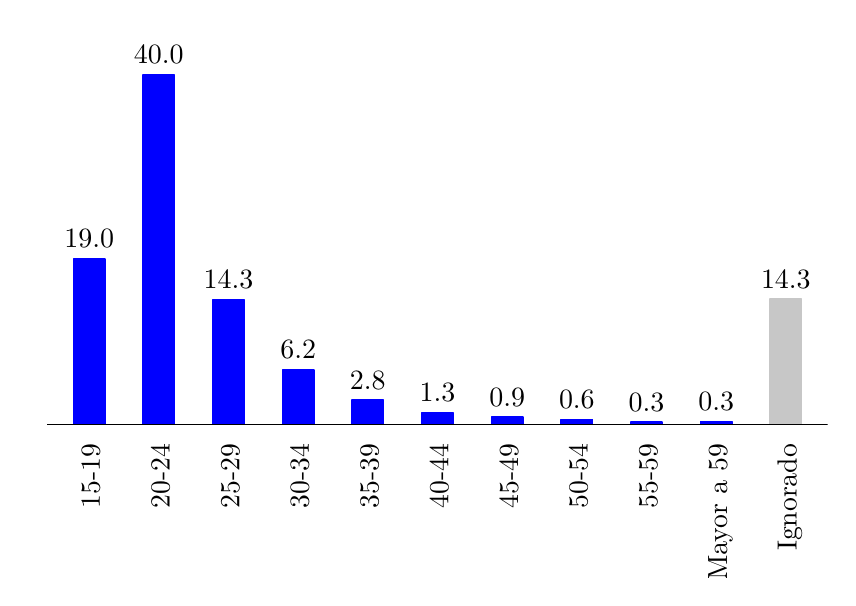
\begin{tikzpicture}[x=1pt,y=1pt]  % Created by tikzDevice version 0.7.0 on 2015-08-28 16:20:10
% !TEX encoding = UTF-8 Unicode
\definecolor[named]{fillColor}{rgb}{1.00,1.00,1.00}
\path[use as bounding box,fill=fillColor,fill opacity=0.00] (0,0) rectangle (289.08,198.74);
\begin{scope}
\path[clip] (  0.00,  0.00) rectangle (289.08,198.74);
\definecolor[named]{drawColor}{rgb}{1.00,1.00,1.00}

\path[draw=drawColor,line width= 0.6pt,line join=round,line cap=round] (  0.00,  0.00) rectangle (289.08,198.74);
\end{scope}
\begin{scope}
\path[clip] (  0.00,  0.00) rectangle (289.08,198.74);

\path[] (  7.11, 55.39) rectangle (289.08,181.67);

\path[] ( 22.22, 55.39) --
	( 22.22,181.67);

\path[] ( 47.39, 55.39) --
	( 47.39,181.67);

\path[] ( 72.57, 55.39) --
	( 72.57,181.67);

\path[] ( 97.75, 55.39) --
	( 97.75,181.67);

\path[] (122.92, 55.39) --
	(122.92,181.67);

\path[] (148.10, 55.39) --
	(148.10,181.67);

\path[] (173.27, 55.39) --
	(173.27,181.67);

\path[] (198.45, 55.39) --
	(198.45,181.67);

\path[] (223.62, 55.39) --
	(223.62,181.67);

\path[] (248.80, 55.39) --
	(248.80,181.67);

\path[] (273.97, 55.39) --
	(273.97,181.67);
\definecolor[named]{drawColor}{rgb}{0.00,0.00,1.00}
\definecolor[named]{fillColor}{rgb}{0.00,0.00,1.00}

\path[draw=drawColor,line width= 0.6pt,line join=round,fill=fillColor] ( 16.55, 55.39) rectangle ( 27.88,115.21);

\path[draw=drawColor,line width= 0.6pt,line join=round,fill=fillColor] ( 41.73, 55.39) rectangle ( 53.06,181.67);

\path[draw=drawColor,line width= 0.6pt,line join=round,fill=fillColor] ( 66.91, 55.39) rectangle ( 78.23,100.50);

\path[draw=drawColor,line width= 0.6pt,line join=round,fill=fillColor] ( 92.08, 55.39) rectangle (103.41, 75.09);

\path[draw=drawColor,line width= 0.6pt,line join=round,fill=fillColor] (117.26, 55.39) rectangle (128.59, 64.15);

\path[draw=drawColor,line width= 0.6pt,line join=round,fill=fillColor] (142.43, 55.39) rectangle (153.76, 59.63);

\path[draw=drawColor,line width= 0.6pt,line join=round,fill=fillColor] (167.61, 55.39) rectangle (178.94, 58.08);

\path[draw=drawColor,line width= 0.6pt,line join=round,fill=fillColor] (192.78, 55.39) rectangle (204.11, 57.21);

\path[draw=drawColor,line width= 0.6pt,line join=round,fill=fillColor] (217.96, 55.39) rectangle (229.29, 56.24);

\path[draw=drawColor,line width= 0.6pt,line join=round,fill=fillColor] (243.13, 55.39) rectangle (254.46, 56.41);
\definecolor[named]{drawColor}{rgb}{0.78,0.78,0.78}
\definecolor[named]{fillColor}{rgb}{0.78,0.78,0.78}

\path[draw=drawColor,line width= 0.6pt,line join=round,fill=fillColor] (268.31, 55.39) rectangle (279.64,100.63);
\definecolor[named]{drawColor}{rgb}{0.00,0.00,0.00}
\definecolor[named]{fillColor}{rgb}{0.00,0.00,0.00}

\path[draw=drawColor,line width= 0.1pt,line join=round,fill=fillColor] (  7.11, 55.39) -- (289.08, 55.39);

\node[text=drawColor,anchor=base,inner sep=0pt, outer sep=0pt, scale=  1.01] at ( 22.22,119.17) {19.0};

\node[text=drawColor,anchor=base,inner sep=0pt, outer sep=0pt, scale=  1.01] at ( 47.39,185.63) {40.0};

\node[text=drawColor,anchor=base,inner sep=0pt, outer sep=0pt, scale=  1.01] at ( 72.57,104.45) {14.3};

\node[text=drawColor,anchor=base,inner sep=0pt, outer sep=0pt, scale=  1.01] at ( 97.75, 79.04) {6.2};

\node[text=drawColor,anchor=base,inner sep=0pt, outer sep=0pt, scale=  1.01] at (122.92, 68.10) {2.8};

\node[text=drawColor,anchor=base,inner sep=0pt, outer sep=0pt, scale=  1.01] at (148.10, 63.59) {1.3};

\node[text=drawColor,anchor=base,inner sep=0pt, outer sep=0pt, scale=  1.01] at (173.27, 62.03) {0.9};

\node[text=drawColor,anchor=base,inner sep=0pt, outer sep=0pt, scale=  1.01] at (198.45, 61.17) {0.6};

\node[text=drawColor,anchor=base,inner sep=0pt, outer sep=0pt, scale=  1.01] at (223.62, 60.20) {0.3};

\node[text=drawColor,anchor=base,inner sep=0pt, outer sep=0pt, scale=  1.01] at (248.80, 60.37) {0.3};

\node[text=drawColor,anchor=base,inner sep=0pt, outer sep=0pt, scale=  1.01] at (273.97,104.59) {14.3};
\end{scope}
\begin{scope}
\path[clip] (  0.00,  0.00) rectangle (289.08,198.74);

\path[] (  7.11, 55.39) --
	(  7.11,181.67);
\end{scope}
\begin{scope}
\path[clip] (  0.00,  0.00) rectangle (289.08,198.74);

\path[] (  7.11, 55.39) --
	(289.08, 55.39);
\end{scope}
\begin{scope}
\path[clip] (  0.00,  0.00) rectangle (289.08,198.74);

\path[] ( 22.22, 51.12) --
	( 22.22, 55.39);

\path[] ( 47.39, 51.12) --
	( 47.39, 55.39);

\path[] ( 72.57, 51.12) --
	( 72.57, 55.39);

\path[] ( 97.75, 51.12) --
	( 97.75, 55.39);

\path[] (122.92, 51.12) --
	(122.92, 55.39);

\path[] (148.10, 51.12) --
	(148.10, 55.39);

\path[] (173.27, 51.12) --
	(173.27, 55.39);

\path[] (198.45, 51.12) --
	(198.45, 55.39);

\path[] (223.62, 51.12) --
	(223.62, 55.39);

\path[] (248.80, 51.12) --
	(248.80, 55.39);

\path[] (273.97, 51.12) --
	(273.97, 55.39);
\end{scope}
\begin{scope}
\path[clip] (  0.00,  0.00) rectangle (289.08,198.74);
\definecolor[named]{drawColor}{rgb}{0.00,0.00,0.00}

\node[text=drawColor,rotate= 90.00,anchor=base east,inner sep=0pt, outer sep=0pt, scale=  1.00] at ( 26.13, 48.28) {15-19};

\node[text=drawColor,rotate= 90.00,anchor=base east,inner sep=0pt, outer sep=0pt, scale=  1.00] at ( 51.30, 48.28) {20-24};

\node[text=drawColor,rotate= 90.00,anchor=base east,inner sep=0pt, outer sep=0pt, scale=  1.00] at ( 76.48, 48.28) {25-29};

\node[text=drawColor,rotate= 90.00,anchor=base east,inner sep=0pt, outer sep=0pt, scale=  1.00] at (101.65, 48.28) {30-34};

\node[text=drawColor,rotate= 90.00,anchor=base east,inner sep=0pt, outer sep=0pt, scale=  1.00] at (126.83, 48.28) {35-39};

\node[text=drawColor,rotate= 90.00,anchor=base east,inner sep=0pt, outer sep=0pt, scale=  1.00] at (152.01, 48.28) {40-44};

\node[text=drawColor,rotate= 90.00,anchor=base east,inner sep=0pt, outer sep=0pt, scale=  1.00] at (177.18, 48.28) {45-49};

\node[text=drawColor,rotate= 90.00,anchor=base east,inner sep=0pt, outer sep=0pt, scale=  1.00] at (202.36, 48.28) {50-54};

\node[text=drawColor,rotate= 90.00,anchor=base east,inner sep=0pt, outer sep=0pt, scale=  1.00] at (227.53, 48.28) {55-59};

\node[text=drawColor,rotate= 90.00,anchor=base east,inner sep=0pt, outer sep=0pt, scale=  1.00] at (252.71, 48.28) {Mayor a  59};

\node[text=drawColor,rotate= 90.00,anchor=base east,inner sep=0pt, outer sep=0pt, scale=  1.00] at (277.88, 48.28) {Ignorado};
\end{scope}
  \end{tikzpicture}}{Instituto Nacional de Estadística, con datos del Ministerio de Educación}

\cajota{Cobertura bruta en los departamentos}{Los departamentos con las menores tasas brutas de cobertura en básico en el 2014 fueron: Alta Verapaz 44.0\%, Huehuetenango  39.9\% y Quiché 39.4\%.
	
	Los departamentos con las más altas tasas brutas de cobertura en básico:  Guatemala 110.4\%, El Progreso 88.7\% y Sacatepequez 86.1\%.}{Tasa bruta de cobertura del ciclo de educación básica}{Por departamento, año 2014, en porcentaje}{\includegraphics[width=52\cuadri]{graficas/basicos/1_10.pdf}}{Instituto Nacional de Estadística, con datos del Ministerio de Educación}

\cajita{Cobertura neta}{La tasa neta de cobertura en básico es la relación que existe entre la parte de la inscripción inicial que se encuentra en la edad escolar de 13 a 15 años y la población de esa misma edad.
	
	 En el año 2009 fue del 40.3\% y en el 2014 fue de 44.9\%, presentando un crecimiento de 4.7 puntos porcentuales.}{Tasa neta de cobertura del ciclo de educación básica}{República de Guatemala, serie histórica, en porcentaje}{\ \\[0mm]\begin{tikzpicture}[x=1pt,y=1pt]  % Created by tikzDevice version 0.7.0 on 2015-08-31 18:25:50
% !TEX encoding = UTF-8 Unicode
\definecolor[named]{fillColor}{rgb}{1.00,1.00,1.00}
\path[use as bounding box,fill=fillColor,fill opacity=0.00] (0,0) rectangle (289.08,198.74);
\begin{scope}
\path[clip] (  0.00,  0.00) rectangle (289.08,198.74);
\definecolor[named]{drawColor}{rgb}{1.00,1.00,1.00}

\path[draw=drawColor,line width= 0.6pt,line join=round,line cap=round] (  0.00,  0.00) rectangle (289.08,198.74);
\end{scope}
\begin{scope}
\path[clip] (  0.00,  0.00) rectangle (289.08,198.74);

\path[] (  1.64, 17.78) rectangle (280.54,191.48);

\path[] (  1.64, 53.87) --
	(280.54, 53.87);

\path[] (  1.64,110.27) --
	(280.54,110.27);

\path[] (  1.64,166.67) --
	(280.54,166.67);

\path[] (  1.64, 25.67) --
	(280.54, 25.67);

\path[] (  1.64, 82.07) --
	(280.54, 82.07);

\path[] (  1.64,138.47) --
	(280.54,138.47);

\path[] ( 33.83, 17.78) --
	( 33.83,191.48);

\path[] ( 87.46, 17.78) --
	( 87.46,191.48);

\path[] (141.09, 17.78) --
	(141.09,191.48);

\path[] (194.73, 17.78) --
	(194.73,191.48);

\path[] (248.36, 17.78) --
	(248.36,191.48);
\definecolor[named]{drawColor}{rgb}{0.00,0.00,1.00}

\path[draw=drawColor,line width= 1.7pt,line join=round] ( 33.83,141.85) --
	( 87.46,171.18) --
	(141.09,176.82) --
	(194.73,174.56) --
	(248.36,183.59);
\definecolor[named]{drawColor}{rgb}{0.00,0.00,0.00}

\node[text=drawColor,anchor=base,inner sep=0pt, outer sep=0pt, scale=  1.01] at ( 33.83,129.98) {40.3};

\node[text=drawColor,anchor=base east,inner sep=0pt, outer sep=0pt, scale=  1.01] at ( 84.34,171.18) {42.9};

\node[text=drawColor,anchor=base,inner sep=0pt, outer sep=0pt, scale=  1.01] at (141.09,180.78) {43.4};

\node[text=drawColor,anchor=base,inner sep=0pt, outer sep=0pt, scale=  1.01] at (194.73,162.69) {43.2};

\node[text=drawColor,anchor=base,inner sep=0pt, outer sep=0pt, scale=  1.01] at (248.36,187.54) {44.0};
\definecolor[named]{fillColor}{rgb}{0.00,0.00,0.00}

\path[draw=drawColor,line width= 0.1pt,line join=round,fill=fillColor] (  1.64, 25.67) -- (280.54, 25.67);
\end{scope}
\begin{scope}
\path[clip] (  0.00,  0.00) rectangle (289.08,198.74);

\path[] (  1.64, 17.78) --
	(  1.64,191.48);
\end{scope}
\begin{scope}
\path[clip] (  0.00,  0.00) rectangle (289.08,198.74);

\path[] (  0.00, 25.67) --
	(  1.64, 25.67);

\path[] (  0.00, 82.07) --
	(  1.64, 82.07);

\path[] (  0.00,138.47) --
	(  1.64,138.47);
\end{scope}
\begin{scope}
\path[clip] (  0.00,  0.00) rectangle (289.08,198.74);

\path[] (  1.64, 17.78) --
	(280.54, 17.78);
\end{scope}
\begin{scope}
\path[clip] (  0.00,  0.00) rectangle (289.08,198.74);

\path[] ( 33.83, 13.51) --
	( 33.83, 17.78);

\path[] ( 87.46, 13.51) --
	( 87.46, 17.78);

\path[] (141.09, 13.51) --
	(141.09, 17.78);

\path[] (194.73, 13.51) --
	(194.73, 17.78);

\path[] (248.36, 13.51) --
	(248.36, 17.78);
\end{scope}
\begin{scope}
\path[clip] (  0.00,  0.00) rectangle (289.08,198.74);
\definecolor[named]{drawColor}{rgb}{0.00,0.00,0.00}

\node[text=drawColor,anchor=base,inner sep=0pt, outer sep=0pt, scale=  1.00] at ( 33.83,  2.85) {2009};

\node[text=drawColor,anchor=base,inner sep=0pt, outer sep=0pt, scale=  1.00] at ( 87.46,  2.85) {2010};

\node[text=drawColor,anchor=base,inner sep=0pt, outer sep=0pt, scale=  1.00] at (141.09,  2.85) {2011};

\node[text=drawColor,anchor=base,inner sep=0pt, outer sep=0pt, scale=  1.00] at (194.73,  2.85) {2012};

\node[text=drawColor,anchor=base,inner sep=0pt, outer sep=0pt, scale=  1.00] at (248.36,  2.85) {2014};
\end{scope}
  \end{tikzpicture}}{Instituto Nacional de Estadística, con datos del Ministerio de Educación}

\cajita{Cobertura neta por sexo}{La tasa neta de cobertura en básico por sexo fue de 46.1\% para hombres y 43.8\% para las mujeres.}{Tasa neta de cobertura del ciclo de educación básica, por sexo}{República de Guatemala, año 2014, en porcentaje}{\ \\[0mm]\begin{tikzpicture}[x=1pt,y=1pt]  % Created by tikzDevice version 0.7.0 on 2015-09-01 14:24:00
% !TEX encoding = UTF-8 Unicode
\definecolor[named]{fillColor}{rgb}{1.00,1.00,1.00}
\path[use as bounding box,fill=fillColor,fill opacity=0.00] (0,0) rectangle (289.08,198.74);
\begin{scope}
\path[clip] (  0.00,  0.00) rectangle (289.08,198.74);
\definecolor[named]{drawColor}{rgb}{1.00,1.00,1.00}

\path[draw=drawColor,line width= 0.6pt,line join=round,line cap=round] (  0.00,  0.00) rectangle (289.08,198.74);
\end{scope}
\begin{scope}
\path[clip] (  0.00,  0.00) rectangle (289.08,198.74);

\path[] (  1.64, 17.78) rectangle (280.54,191.48);

\path[] (  1.64, 47.21) --
	(280.54, 47.21);

\path[] (  1.64, 90.30) --
	(280.54, 90.30);

\path[] (  1.64,133.39) --
	(280.54,133.39);

\path[] (  1.64,176.48) --
	(280.54,176.48);

\path[] (  1.64, 25.67) --
	(280.54, 25.67);

\path[] (  1.64, 68.76) --
	(280.54, 68.76);

\path[] (  1.64,111.85) --
	(280.54,111.85);

\path[] (  1.64,154.93) --
	(280.54,154.93);

\path[] ( 33.83, 17.78) --
	( 33.83,191.48);

\path[] ( 87.46, 17.78) --
	( 87.46,191.48);

\path[] (141.09, 17.78) --
	(141.09,191.48);

\path[] (194.73, 17.78) --
	(194.73,191.48);

\path[] (248.36, 17.78) --
	(248.36,191.48);
\definecolor[named]{drawColor}{rgb}{0.00,0.00,1.00}

\path[draw=drawColor,line width= 1.7pt,line join=round] ( 33.83, 96.77) --
	( 87.46,123.48) --
	(141.09,133.39) --
	(194.73,167.64) --
	(248.36,183.59);
\definecolor[named]{drawColor}{rgb}{0.00,0.00,0.00}

\node[text=drawColor,anchor=base,inner sep=0pt, outer sep=0pt, scale=  1.01] at ( 33.83, 84.90) {53.0};

\node[text=drawColor,anchor=base east,inner sep=0pt, outer sep=0pt, scale=  1.01] at ( 84.34,123.48) {65.4};

\node[text=drawColor,anchor=base east,inner sep=0pt, outer sep=0pt, scale=  1.01] at (137.98,133.39) {70.0};

\node[text=drawColor,anchor=base east,inner sep=0pt, outer sep=0pt, scale=  1.01] at (191.61,167.64) {85.9};

\node[text=drawColor,anchor=base,inner sep=0pt, outer sep=0pt, scale=  1.01] at (248.36,187.54) {93.3};
\definecolor[named]{fillColor}{rgb}{0.00,0.00,0.00}

\path[draw=drawColor,line width= 0.1pt,line join=round,fill=fillColor] (  1.64, 25.67) -- (280.54, 25.67);
\end{scope}
\begin{scope}
\path[clip] (  0.00,  0.00) rectangle (289.08,198.74);

\path[] (  1.64, 17.78) --
	(  1.64,191.48);
\end{scope}
\begin{scope}
\path[clip] (  0.00,  0.00) rectangle (289.08,198.74);

\path[] (  0.00, 25.67) --
	(  1.64, 25.67);

\path[] (  0.00, 68.76) --
	(  1.64, 68.76);

\path[] (  0.00,111.85) --
	(  1.64,111.85);

\path[] (  0.00,154.93) --
	(  1.64,154.93);
\end{scope}
\begin{scope}
\path[clip] (  0.00,  0.00) rectangle (289.08,198.74);

\path[] (  1.64, 17.78) --
	(280.54, 17.78);
\end{scope}
\begin{scope}
\path[clip] (  0.00,  0.00) rectangle (289.08,198.74);

\path[] ( 33.83, 13.51) --
	( 33.83, 17.78);

\path[] ( 87.46, 13.51) --
	( 87.46, 17.78);

\path[] (141.09, 13.51) --
	(141.09, 17.78);

\path[] (194.73, 13.51) --
	(194.73, 17.78);

\path[] (248.36, 13.51) --
	(248.36, 17.78);
\end{scope}
\begin{scope}
\path[clip] (  0.00,  0.00) rectangle (289.08,198.74);
\definecolor[named]{drawColor}{rgb}{0.00,0.00,0.00}

\node[text=drawColor,anchor=base,inner sep=0pt, outer sep=0pt, scale=  1.00] at ( 33.83,  2.85) {1987};

\node[text=drawColor,anchor=base,inner sep=0pt, outer sep=0pt, scale=  1.00] at ( 87.46,  2.85) {1995};

\node[text=drawColor,anchor=base,inner sep=0pt, outer sep=0pt, scale=  1.00] at (141.09,  2.85) {1998/99};

\node[text=drawColor,anchor=base,inner sep=0pt, outer sep=0pt, scale=  1.00] at (194.73,  2.85) {2002};

\node[text=drawColor,anchor=base,inner sep=0pt, outer sep=0pt, scale=  1.00] at (248.36,  2.85) {2008/09};
\end{scope}
  \end{tikzpicture}}{Instituto Nacional de Estadística, con datos del Ministerio de Educación}

\cajota{Cobertura neta en los departamentos}{Los departamentos con las menores tasas  netas de cobertura en básico en el 2014 fueron: Huehuetenango 26.1\%, Quiché 24.7\% y Alta Verapaz 24.4\%.
	
	 Los departamentos con las mayores tasas netas de cobertura en básico fueron: Guatemala 72.5\%, El Progreso 60.5\% y Sacatepéquez 58.4\%.}{Tasa neta de cobertura del ciclo de educación básica}{Por departamento, año 2014, en porcentaje}{\includegraphics[width=52\cuadri]{graficas/basicos/1_13.pdf}}{Instituto Nacional de Estadística, con datos del Ministerio de Educación}




\cajita{Repitencia}{La tasa de repitencia en básico es la relación que existe entre el número de repitentes y el número de alumnos que en el año  estaban inscritos en el mismo grado.
	
	En el año 2009 el 3.1\% y en el año 2014 fue de 4.0\%, presentando un crecimiento de 0.9 puntos porcentuales.}{Tasa de repitencia del ciclo de educación básica}{República de Guatemala, serie histórica, en porcentaje}{\ \\[0mm]\begin{tikzpicture}[x=1pt,y=1pt]  % Created by tikzDevice version 0.10.1 on 2016-02-29 12:51:49
% !TEX encoding = UTF-8 Unicode
\definecolor{fillColor}{RGB}{255,255,255}
\path[use as bounding box,fill=fillColor,fill opacity=0.00] (0,0) rectangle (289.08,198.74);
\begin{scope}
\path[clip] (  0.00,  0.00) rectangle (289.08,198.74);

\path[] (  0.00,  0.00) rectangle (289.08,198.74);
\end{scope}
\begin{scope}
\path[clip] (  0.00,  0.00) rectangle (289.08,198.74);

\path[] ( -4.90, 15.61) rectangle (280.54,191.48);

\path[] (  0.00, 52.00) --
	(280.54, 52.00);

\path[] (  0.00,108.80) --
	(280.54,108.80);

\path[] (  0.00,165.60) --
	(280.54,165.60);

\path[] (  0.00, 23.61) --
	(280.54, 23.61);

\path[] (  0.00, 80.40) --
	(280.54, 80.40);

\path[] (  0.00,137.20) --
	(280.54,137.20);

\path[] ( 22.73, 15.61) --
	( 22.73,191.48);

\path[] ( 68.76, 15.61) --
	( 68.76,191.48);

\path[] (114.80, 15.61) --
	(114.80,191.48);

\path[] (160.84, 15.61) --
	(160.84,191.48);

\path[] (206.88, 15.61) --
	(206.88,191.48);

\path[] (252.92, 15.61) --
	(252.92,191.48);
\definecolor{drawColor}{RGB}{0,0,255}

\path[draw=drawColor,line width= 1.7pt,line join=round] ( 22.73,110.51) --
	( 68.76,107.67) --
	(114.80,103.12) --
	(160.84,183.49) --
	(206.88,152.53) --
	(252.92,138.34);
\definecolor{drawColor}{RGB}{0,0,0}

\node[text=drawColor,anchor=base,inner sep=0pt, outer sep=0pt, scale=  1.02] at ( 22.73,114.48) {3.1};

\node[text=drawColor,anchor=base west,inner sep=0pt, outer sep=0pt, scale=  1.02] at ( 68.76,111.64) {3.0};

\node[text=drawColor,anchor=base,inner sep=0pt, outer sep=0pt, scale=  1.02] at (114.80, 91.21) {2.8};

\node[text=drawColor,anchor=base,inner sep=0pt, outer sep=0pt, scale=  1.02] at (160.84,187.46) {5.6};

\node[text=drawColor,anchor=base west,inner sep=0pt, outer sep=0pt, scale=  1.02] at (206.88,156.51) {4.5};

\node[text=drawColor,anchor=base,inner sep=0pt, outer sep=0pt, scale=  1.02] at (252.92,126.42) {4.0};

\path[draw=drawColor,line width= 0.1pt,line join=round] (  0.00, 23.61) -- (280.54, 23.61);

\path[] ( -4.90, 15.61) rectangle (280.54,191.48);
\end{scope}
\begin{scope}
\path[clip] (  0.00,  0.00) rectangle (289.08,198.74);

\path[] (  0.00, 15.61) --
	(280.54, 15.61);
\end{scope}
\begin{scope}
\path[clip] (  0.00,  0.00) rectangle (289.08,198.74);

\path[] ( 22.73, 12.86) --
	( 22.73, 15.61);

\path[] ( 68.76, 12.86) --
	( 68.76, 15.61);

\path[] (114.80, 12.86) --
	(114.80, 15.61);

\path[] (160.84, 12.86) --
	(160.84, 15.61);

\path[] (206.88, 12.86) --
	(206.88, 15.61);

\path[] (252.92, 12.86) --
	(252.92, 15.61);
\end{scope}
\begin{scope}
\path[clip] (  0.00,  0.00) rectangle (289.08,198.74);
\definecolor{drawColor}{RGB}{0,0,0}

\node[text=drawColor,anchor=base,inner sep=0pt, outer sep=0pt, scale=  1.00] at ( 22.73,  2.85) {2009};

\node[text=drawColor,anchor=base,inner sep=0pt, outer sep=0pt, scale=  1.00] at ( 68.76,  2.85) {2010};

\node[text=drawColor,anchor=base,inner sep=0pt, outer sep=0pt, scale=  1.00] at (114.80,  2.85) {2011};

\node[text=drawColor,anchor=base,inner sep=0pt, outer sep=0pt, scale=  1.00] at (160.84,  2.85) {2012};

\node[text=drawColor,anchor=base,inner sep=0pt, outer sep=0pt, scale=  1.00] at (206.88,  2.85) {2013};

\node[text=drawColor,anchor=base,inner sep=0pt, outer sep=0pt, scale=  1.00] at (252.92,  2.85) {2014};
\end{scope}
  \end{tikzpicture}}{Instituto Nacional de Estadística, con datos del Ministerio de Educación}

\cajita{Repitencia por sexo}{La tasa de repitencia en básico por sexo fue del 4.3\% para hombres y 3.7\% para las mujeres.}{Tasa de repitencia del ciclo de educación básica, por sexo}{República de Guatemala, año 2014, en porcentaje}{\ \\[0mm]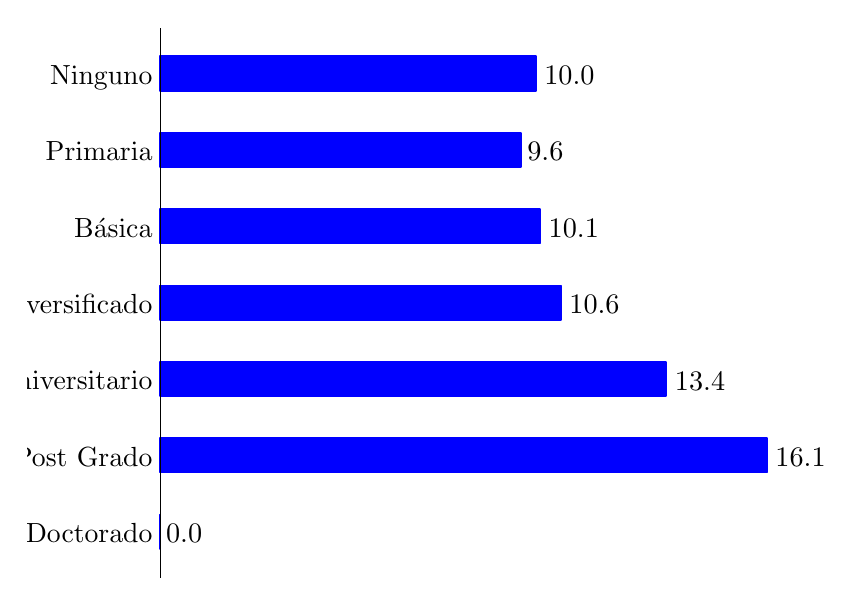
\begin{tikzpicture}[x=1pt,y=1pt]  % Created by tikzDevice version 0.10.1 on 2016-02-29 14:42:48
% !TEX encoding = UTF-8 Unicode
\definecolor{fillColor}{RGB}{255,255,255}
\path[use as bounding box,fill=fillColor,fill opacity=0.00] (0,0) rectangle (289.08,198.74);
\begin{scope}
\path[clip] (  0.00,  0.00) rectangle (289.08,198.74);

\path[] (  0.00,  0.00) rectangle (289.08,198.74);
\end{scope}
\begin{scope}
\path[clip] (  0.00,  0.00) rectangle (289.08,198.74);

\path[] ( 47.80,  0.00) rectangle (267.09,198.74);

\path[] ( 47.80, 16.56) --
	(267.09, 16.56);

\path[] ( 47.80, 44.16) --
	(267.09, 44.16);

\path[] ( 47.80, 71.77) --
	(267.09, 71.77);

\path[] ( 47.80, 99.37) --
	(267.09, 99.37);

\path[] ( 47.80,126.97) --
	(267.09,126.97);

\path[] ( 47.80,154.58) --
	(267.09,154.58);

\path[] ( 47.80,182.18) --
	(267.09,182.18);
\definecolor{drawColor}{RGB}{0,0,255}
\definecolor{fillColor}{RGB}{0,0,255}

\path[draw=drawColor,line width= 0.6pt,line join=round,fill=fillColor] ( 47.80, 10.35) rectangle ( 47.80, 22.77);

\path[draw=drawColor,line width= 0.6pt,line join=round,fill=fillColor] ( 47.80, 37.95) rectangle (267.09, 50.38);

\path[draw=drawColor,line width= 0.6pt,line join=round,fill=fillColor] ( 47.80, 65.56) rectangle (230.77, 77.98);

\path[draw=drawColor,line width= 0.6pt,line join=round,fill=fillColor] ( 47.80, 93.16) rectangle (192.63,105.58);

\path[draw=drawColor,line width= 0.6pt,line join=round,fill=fillColor] ( 47.80,120.76) rectangle (185.14,133.19);

\path[draw=drawColor,line width= 0.6pt,line join=round,fill=fillColor] ( 47.80,148.37) rectangle (178.32,160.79);

\path[draw=drawColor,line width= 0.6pt,line join=round,fill=fillColor] ( 47.80,175.97) rectangle (183.58,188.39);
\definecolor{drawColor}{RGB}{0,0,0}

\path[draw=drawColor,line width= 0.1pt,line join=round] ( 47.80,  0.00) -- ( 47.80,198.74);

\node[text=drawColor,anchor=base west,inner sep=0pt, outer sep=0pt, scale=  1.02] at ( 50.03, 12.59) {0.0};

\node[text=drawColor,anchor=base west,inner sep=0pt, outer sep=0pt, scale=  1.02] at (270.21, 40.19) {16.1};

\node[text=drawColor,anchor=base west,inner sep=0pt, outer sep=0pt, scale=  1.02] at (233.89, 67.80) {13.4};

\node[text=drawColor,anchor=base west,inner sep=0pt, outer sep=0pt, scale=  1.02] at (195.76, 95.40) {10.6};

\node[text=drawColor,anchor=base west,inner sep=0pt, outer sep=0pt, scale=  1.02] at (188.27,123.00) {10.1};

\node[text=drawColor,anchor=base west,inner sep=0pt, outer sep=0pt, scale=  1.02] at (180.56,150.61) {9.6};

\node[text=drawColor,anchor=base west,inner sep=0pt, outer sep=0pt, scale=  1.02] at (186.71,178.21) {10.0};

\path[] ( 47.80,  0.00) rectangle (267.09,198.74);
\end{scope}
\begin{scope}
\path[clip] (  0.00,  0.00) rectangle (289.08,198.74);

\path[] ( 47.80,  0.00) --
	( 47.80,198.74);
\end{scope}
\begin{scope}
\path[clip] (  0.00,  0.00) rectangle (289.08,198.74);
\definecolor{drawColor}{RGB}{0,0,0}

\node[text=drawColor,anchor=base east,inner sep=0pt, outer sep=0pt, scale=  1.00] at ( 45.05, 12.65) {Doctorado};

\node[text=drawColor,anchor=base east,inner sep=0pt, outer sep=0pt, scale=  1.00] at ( 45.05, 40.26) {Post Grado};

\node[text=drawColor,anchor=base east,inner sep=0pt, outer sep=0pt, scale=  1.00] at ( 45.05, 67.86) {Universitario};

\node[text=drawColor,anchor=base east,inner sep=0pt, outer sep=0pt, scale=  1.00] at ( 45.05, 95.46) {Diversificado};

\node[text=drawColor,anchor=base east,inner sep=0pt, outer sep=0pt, scale=  1.00] at ( 45.05,123.07) {Básica};

\node[text=drawColor,anchor=base east,inner sep=0pt, outer sep=0pt, scale=  1.00] at ( 45.05,150.67) {Primaria};

\node[text=drawColor,anchor=base east,inner sep=0pt, outer sep=0pt, scale=  1.00] at ( 45.05,178.27) {Ninguno};
\end{scope}
\begin{scope}
\path[clip] (  0.00,  0.00) rectangle (289.08,198.74);

\path[] ( 45.05, 16.56) --
	( 47.80, 16.56);

\path[] ( 45.05, 44.16) --
	( 47.80, 44.16);

\path[] ( 45.05, 71.77) --
	( 47.80, 71.77);

\path[] ( 45.05, 99.37) --
	( 47.80, 99.37);

\path[] ( 45.05,126.97) --
	( 47.80,126.97);

\path[] ( 45.05,154.58) --
	( 47.80,154.58);

\path[] ( 45.05,182.18) --
	( 47.80,182.18);
\end{scope}
  \end{tikzpicture}}{Instituto Nacional de Estadística, con datos del Ministerio de Educación}

\cajota{Repitencia en los departamentos}{Los departamentos con las menores tasas de repitencia en básico en el 2013 fueron: Retalhuleu 2.2\%, Petén 2.0\% y Jutiapa 1.7\%.
	
	 Los departamentos con las mayores tasas de repitencia en básico fueron: Sacatepéquez 8.0\%, Sololá 6.8\% y Totonicapán 5.7\%. El departamento de Guatemala presentó una tasa de repitencia de 4.3\%.}{Tasa de repitencia del ciclo de educación básica}{Por departamento, año 2014, en porcentaje}{\includegraphics[width=52\cuadri]{graficas/basicos/1_16.pdf}}{Instituto Nacional de Estadística, con datos del Ministerio de Educación}






\cajita{Sobre-edad}{La tasa de sobre-edad en básico es la relación que existe entre la cantidad de alumnos inscritos en los diferentes grados de un nivel educativo, con dos o más años de atraso escolar por encima de la edad correspondiente al grado de estudio.
	
	En el año 2009 fue del 34\% y en el año 2014 fue de 23.6\%, el cual fue una disminución de  10.4 puntos porcentuales.}{Tasa de sobre-edad del ciclo de educación básica}{República de Guatemala, serie histórica, en porcentaje}{\ \\[0mm]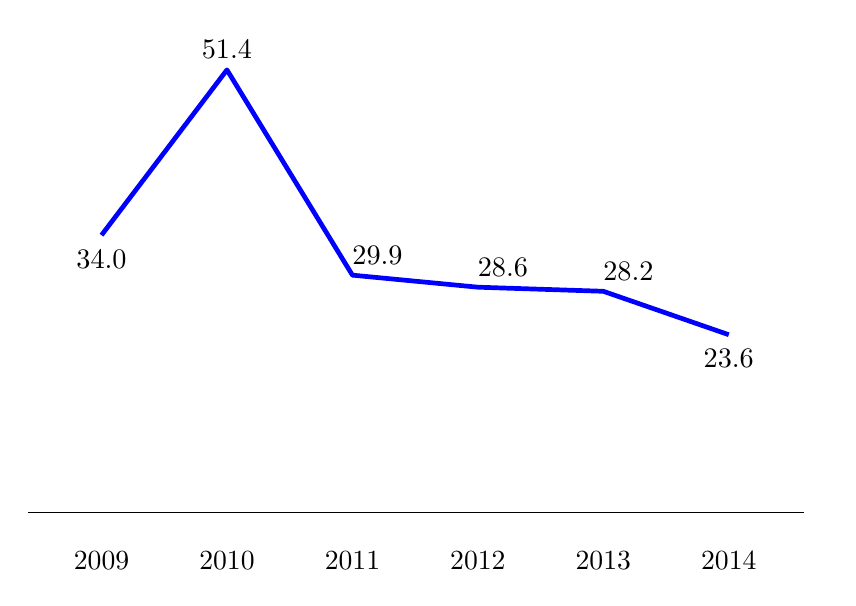
\begin{tikzpicture}[x=1pt,y=1pt]  % Created by tikzDevice version 0.10.1 on 2016-02-29 12:52:16
% !TEX encoding = UTF-8 Unicode
\definecolor{fillColor}{RGB}{255,255,255}
\path[use as bounding box,fill=fillColor,fill opacity=0.00] (0,0) rectangle (289.08,198.74);
\begin{scope}
\path[clip] (  0.00,  0.00) rectangle (289.08,198.74);

\path[] (  0.00,  0.00) rectangle (289.08,198.74);
\end{scope}
\begin{scope}
\path[clip] (  0.00,  0.00) rectangle (289.08,198.74);

\path[] ( -0.52, 15.61) rectangle (280.54,191.48);

\path[] (  0.00, 23.61) --
	(280.54, 23.61);

\path[] (  0.00, 58.09) --
	(280.54, 58.09);

\path[] (  0.00, 92.58) --
	(280.54, 92.58);

\path[] (  0.00,127.07) --
	(280.54,127.07);

\path[] (  0.00,161.56) --
	(280.54,161.56);

\path[] (  0.00, 40.85) --
	(280.54, 40.85);

\path[] (  0.00, 75.34) --
	(280.54, 75.34);

\path[] (  0.00,109.82) --
	(280.54,109.82);

\path[] (  0.00,144.31) --
	(280.54,144.31);

\path[] (  0.00,178.80) --
	(280.54,178.80);

\path[] ( 26.68, 15.61) --
	( 26.68,191.48);

\path[] ( 72.01, 15.61) --
	( 72.01,191.48);

\path[] (117.35, 15.61) --
	(117.35,191.48);

\path[] (162.68, 15.61) --
	(162.68,191.48);

\path[] (208.01, 15.61) --
	(208.01,191.48);

\path[] (253.34, 15.61) --
	(253.34,191.48);
\definecolor{drawColor}{RGB}{0,0,255}

\path[draw=drawColor,line width= 1.7pt,line join=round] ( 26.68,123.76) --
	( 72.01,183.49) --
	(117.35,109.31) --
	(162.68,104.96) --
	(208.01,103.48) --
	(253.34, 87.79);
\definecolor{drawColor}{RGB}{0,0,0}

\node[text=drawColor,anchor=base,inner sep=0pt, outer sep=0pt, scale=  1.02] at ( 26.68,111.84) {34.0};

\node[text=drawColor,anchor=base,inner sep=0pt, outer sep=0pt, scale=  1.02] at ( 72.01,187.46) {51.4};

\node[text=drawColor,anchor=base west,inner sep=0pt, outer sep=0pt, scale=  1.02] at (117.35,113.28) {29.9};

\node[text=drawColor,anchor=base west,inner sep=0pt, outer sep=0pt, scale=  1.02] at (162.68,108.93) {28.6};

\node[text=drawColor,anchor=base west,inner sep=0pt, outer sep=0pt, scale=  1.02] at (208.01,107.45) {28.2};

\node[text=drawColor,anchor=base,inner sep=0pt, outer sep=0pt, scale=  1.02] at (253.34, 75.87) {23.6};

\path[draw=drawColor,line width= 0.1pt,line join=round] (  0.00, 23.61) -- (280.54, 23.61);

\path[] ( -0.52, 15.61) rectangle (280.54,191.48);
\end{scope}
\begin{scope}
\path[clip] (  0.00,  0.00) rectangle (289.08,198.74);

\path[] (  0.00, 15.61) --
	(280.54, 15.61);
\end{scope}
\begin{scope}
\path[clip] (  0.00,  0.00) rectangle (289.08,198.74);

\path[] ( 26.68, 12.86) --
	( 26.68, 15.61);

\path[] ( 72.01, 12.86) --
	( 72.01, 15.61);

\path[] (117.35, 12.86) --
	(117.35, 15.61);

\path[] (162.68, 12.86) --
	(162.68, 15.61);

\path[] (208.01, 12.86) --
	(208.01, 15.61);

\path[] (253.34, 12.86) --
	(253.34, 15.61);
\end{scope}
\begin{scope}
\path[clip] (  0.00,  0.00) rectangle (289.08,198.74);
\definecolor{drawColor}{RGB}{0,0,0}

\node[text=drawColor,anchor=base,inner sep=0pt, outer sep=0pt, scale=  1.00] at ( 26.68,  2.85) {2009};

\node[text=drawColor,anchor=base,inner sep=0pt, outer sep=0pt, scale=  1.00] at ( 72.01,  2.85) {2010};

\node[text=drawColor,anchor=base,inner sep=0pt, outer sep=0pt, scale=  1.00] at (117.35,  2.85) {2011};

\node[text=drawColor,anchor=base,inner sep=0pt, outer sep=0pt, scale=  1.00] at (162.68,  2.85) {2012};

\node[text=drawColor,anchor=base,inner sep=0pt, outer sep=0pt, scale=  1.00] at (208.01,  2.85) {2013};

\node[text=drawColor,anchor=base,inner sep=0pt, outer sep=0pt, scale=  1.00] at (253.34,  2.85) {2014};
\end{scope}
  \end{tikzpicture}}{Instituto Nacional de Estadística, con datos del Ministerio de Educación}

\cajita{Sobre-edad por sexo}{La tasa de sobre-edad en básico por sexo en el 2014 fue de 26.5\% para hombres y 20.3\% para las mujeres.}{Tasa de sobre-edad del ciclo de educación básica, por sexo}{República de Guatemala, año 2014, en porcentaje}{\ \\[0mm]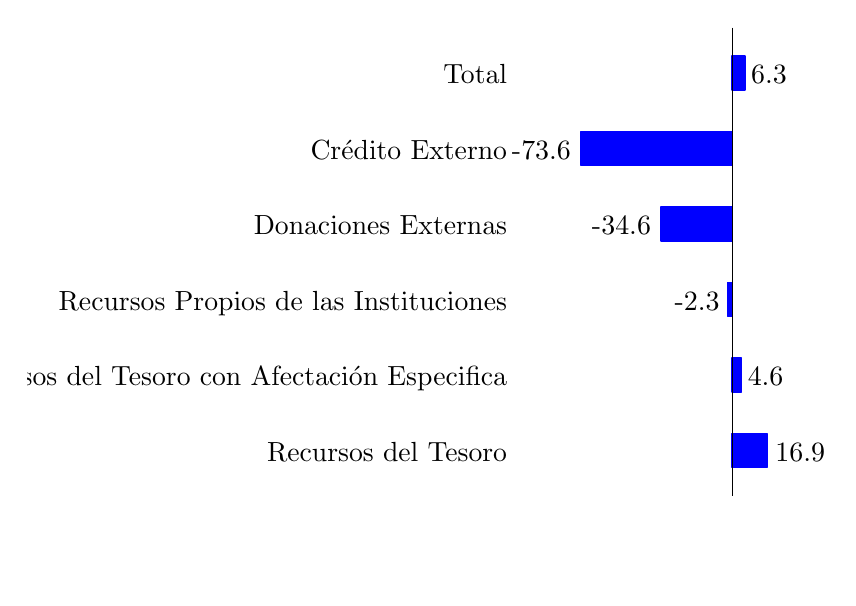
\begin{tikzpicture}[x=1pt,y=1pt]  % Created by tikzDevice version 0.7.0 on 2015-08-28 16:35:09
% !TEX encoding = UTF-8 Unicode
\definecolor[named]{fillColor}{rgb}{1.00,1.00,1.00}
\path[use as bounding box,fill=fillColor,fill opacity=0.00] (0,0) rectangle (289.08,198.74);
\begin{scope}
\path[clip] (  0.00,  0.00) rectangle (289.08,198.74);
\definecolor[named]{drawColor}{rgb}{1.00,1.00,1.00}

\path[draw=drawColor,line width= 0.6pt,line join=round,line cap=round] (  0.00,  0.00) rectangle (289.08,198.74);
\end{scope}
\begin{scope}
\path[clip] (  0.00,  0.00) rectangle (289.08,198.74);

\path[] (199.99, 29.60) rectangle (267.09,198.74);

\path[] (199.99, 45.97) --
	(267.09, 45.97);

\path[] (199.99, 73.25) --
	(267.09, 73.25);

\path[] (199.99,100.53) --
	(267.09,100.53);

\path[] (199.99,127.81) --
	(267.09,127.81);

\path[] (199.99,155.09) --
	(267.09,155.09);

\path[] (199.99,182.37) --
	(267.09,182.37);
\definecolor[named]{drawColor}{rgb}{0.00,0.00,1.00}
\definecolor[named]{fillColor}{rgb}{0.00,0.00,1.00}

\path[draw=drawColor,line width= 0.6pt,line join=round,fill=fillColor] (254.56, 39.83) rectangle (267.09, 52.11);

\path[draw=drawColor,line width= 0.6pt,line join=round,fill=fillColor] (254.56, 67.11) rectangle (257.97, 79.39);

\path[draw=drawColor,line width= 0.6pt,line join=round,fill=fillColor] (252.85, 94.39) rectangle (254.56,106.67);

\path[draw=drawColor,line width= 0.6pt,line join=round,fill=fillColor] (228.90,121.67) rectangle (254.56,133.95);

\path[draw=drawColor,line width= 0.6pt,line join=round,fill=fillColor] (199.99,148.95) rectangle (254.56,161.23);

\path[draw=drawColor,line width= 0.6pt,line join=round,fill=fillColor] (254.56,176.24) rectangle (259.23,188.51);
\definecolor[named]{drawColor}{rgb}{0.00,0.00,0.00}
\definecolor[named]{fillColor}{rgb}{0.00,0.00,0.00}

\path[draw=drawColor,line width= 0.1pt,line join=round,fill=fillColor] (254.56, 29.60) -- (254.56,198.74);

\node[text=drawColor,anchor=base west,inner sep=0pt, outer sep=0pt, scale=  1.01] at (270.20, 42.01) {16.9};

\node[text=drawColor,anchor=base west,inner sep=0pt, outer sep=0pt, scale=  1.01] at (260.20, 69.29) {4.6};

\node[text=drawColor,anchor=base east,inner sep=0pt, outer sep=0pt, scale=  1.01] at (250.06, 96.57) {-2.3};

\node[text=drawColor,anchor=base east,inner sep=0pt, outer sep=0pt, scale=  1.01] at (225.23,123.86) {-34.6};

\node[text=drawColor,anchor=base east,inner sep=0pt, outer sep=0pt, scale=  1.01] at (196.31,151.14) {-73.6};

\node[text=drawColor,anchor=base west,inner sep=0pt, outer sep=0pt, scale=  1.01] at (261.46,178.42) {6.3};
\end{scope}
\begin{scope}
\path[clip] (  0.00,  0.00) rectangle (289.08,198.74);

\path[] (199.99, 29.60) --
	(199.99,198.74);
\end{scope}
\begin{scope}
\path[clip] (  0.00,  0.00) rectangle (289.08,198.74);
\definecolor[named]{drawColor}{rgb}{0.00,0.00,0.00}

\node[text=drawColor,anchor=base east,inner sep=0pt, outer sep=0pt, scale=  1.00] at (173.23, 42.06) {Recursos del Tesoro};

\node[text=drawColor,anchor=base east,inner sep=0pt, outer sep=0pt, scale=  1.00] at (173.23, 69.34) {Recursos del Tesoro con Afectaci\'on Especifica};

\node[text=drawColor,anchor=base east,inner sep=0pt, outer sep=0pt, scale=  1.00] at (173.23, 96.62) {Recursos Propios de las Instituciones};

\node[text=drawColor,anchor=base east,inner sep=0pt, outer sep=0pt, scale=  1.00] at (173.23,123.90) {Donaciones Externas};

\node[text=drawColor,anchor=base east,inner sep=0pt, outer sep=0pt, scale=  1.00] at (173.23,151.18) {Cr\'edito Externo};

\node[text=drawColor,anchor=base east,inner sep=0pt, outer sep=0pt, scale=  1.00] at (173.23,178.47) {Total};
\end{scope}
\begin{scope}
\path[clip] (  0.00,  0.00) rectangle (289.08,198.74);

\path[] (173.23, 45.97) --
	(177.50, 45.97);

\path[] (173.23, 73.25) --
	(177.50, 73.25);

\path[] (173.23,100.53) --
	(177.50,100.53);

\path[] (173.23,127.81) --
	(177.50,127.81);

\path[] (173.23,155.09) --
	(177.50,155.09);

\path[] (173.23,182.37) --
	(177.50,182.37);
\end{scope}
\begin{scope}
\path[clip] (  0.00,  0.00) rectangle (289.08,198.74);

\path[] (199.99, 29.60) --
	(267.09, 29.60);
\end{scope}
  \end{tikzpicture}}{Instituto Nacional de Estadística, con datos del Ministerio de Educación}

\cajota{Sobre-edad en los departamentos}{El mapa muestra en color celeste los departamentos con las menores tasas de sobre-edad en básico fueron: Totonicapán 19.0\%, Chimaltenango 17.8\% y Quetzaltenango 15.6\%.
	
	 Los departamentos con las mayores tasas  de sobre-edad en básico: Alta Verapaz 37.6\%, Petén 28.1\% y Quiché 27.5\%.
	 
	 El departamento de Guatemala tuvo un 24.8\%.}{Tasa de sobre-edad del ciclo de educación básica}{Por departamento, año 2014, en porcentaje}{\includegraphics[width=52\cuadri]{graficas/basicos/1_19.pdf}}{Instituto Nacional de Estadística, con datos del Ministerio de Educación}





\cajita{Deserción}{La tasa de deserción en básico se refiere a la cantidad de alumnos que no concluyen el ciclo lectivo.
	
	En el año fue 2009 el 8.2\% y en el año 2014 fue de 4.1\%, que fue una disminución de 4.1 puntos porcentuales.}{Tasa de deserción del ciclo de educación básica}{República de Guatemala, serie histórica, en porcentaje}{\ \\[0mm]\begin{tikzpicture}[x=1pt,y=1pt]  % Created by tikzDevice version 0.7.0 on 2015-08-31 18:28:05
% !TEX encoding = UTF-8 Unicode
\definecolor[named]{fillColor}{rgb}{1.00,1.00,1.00}
\path[use as bounding box,fill=fillColor,fill opacity=0.00] (0,0) rectangle (289.08,198.74);
\begin{scope}
\path[clip] (  0.00,  0.00) rectangle (289.08,198.74);
\definecolor[named]{drawColor}{rgb}{1.00,1.00,1.00}

\path[draw=drawColor,line width= 0.6pt,line join=round,line cap=round] (  0.00,  0.00) rectangle (289.08,198.74);
\end{scope}
\begin{scope}
\path[clip] (  0.00,  0.00) rectangle (289.08,198.74);

\path[] (  8.28, 17.78) rectangle (280.54,191.48);

\path[] (  8.28, 44.84) --
	(280.54, 44.84);

\path[] (  8.28, 83.16) --
	(280.54, 83.16);

\path[] (  8.28,121.49) --
	(280.54,121.49);

\path[] (  8.28,159.82) --
	(280.54,159.82);

\path[] (  8.28, 25.67) --
	(280.54, 25.67);

\path[] (  8.28, 64.00) --
	(280.54, 64.00);

\path[] (  8.28,102.33) --
	(280.54,102.33);

\path[] (  8.28,140.66) --
	(280.54,140.66);

\path[] (  8.28,178.99) --
	(280.54,178.99);

\path[] ( 39.69, 17.78) --
	( 39.69,191.48);

\path[] ( 92.05, 17.78) --
	( 92.05,191.48);

\path[] (144.41, 17.78) --
	(144.41,191.48);

\path[] (196.77, 17.78) --
	(196.77,191.48);

\path[] (249.13, 17.78) --
	(249.13,191.48);
\definecolor[named]{drawColor}{rgb}{0.00,0.00,1.00}

\path[draw=drawColor,line width= 1.7pt,line join=round] ( 39.69,151.39) --
	( 92.05,183.59) --
	(144.41,105.40) --
	(196.77,131.46) --
	(249.13,116.13);
\definecolor[named]{drawColor}{rgb}{0.00,0.00,0.00}

\node[text=drawColor,anchor=base,inner sep=0pt, outer sep=0pt, scale=  1.01] at ( 39.69,139.52) {8.2};

\node[text=drawColor,anchor=base,inner sep=0pt, outer sep=0pt, scale=  1.01] at ( 92.05,187.54) {10.3};

\node[text=drawColor,anchor=base,inner sep=0pt, outer sep=0pt, scale=  1.01] at (144.41, 93.53) {5.2};

\node[text=drawColor,anchor=base,inner sep=0pt, outer sep=0pt, scale=  1.01] at (196.77,135.42) {6.9};

\node[text=drawColor,anchor=base,inner sep=0pt, outer sep=0pt, scale=  1.01] at (249.13,104.26) {5.9};
\definecolor[named]{fillColor}{rgb}{0.00,0.00,0.00}

\path[draw=drawColor,line width= 0.1pt,line join=round,fill=fillColor] (  8.28, 25.67) -- (280.54, 25.67);
\end{scope}
\begin{scope}
\path[clip] (  0.00,  0.00) rectangle (289.08,198.74);

\path[] (  8.28, 17.78) --
	(  8.28,191.48);
\end{scope}
\begin{scope}
\path[clip] (  0.00,  0.00) rectangle (289.08,198.74);
\definecolor[named]{drawColor}{rgb}{1.00,1.00,1.00}

\node[text=drawColor,text opacity=0.00,anchor=base east,inner sep=0pt, outer sep=0pt, scale=  1.00] at (  1.17, 21.76) {0.0};

\node[text=drawColor,text opacity=0.00,anchor=base east,inner sep=0pt, outer sep=0pt, scale=  1.00] at (  1.17, 60.09) {2.5};

\node[text=drawColor,text opacity=0.00,anchor=base east,inner sep=0pt, outer sep=0pt, scale=  1.00] at (  1.17, 98.42) {5.0};

\node[text=drawColor,text opacity=0.00,anchor=base east,inner sep=0pt, outer sep=0pt, scale=  1.00] at (  1.17,136.75) {7.5};

\node[text=drawColor,text opacity=0.00,anchor=base east,inner sep=0pt, outer sep=0pt, scale=  1.00] at (  1.17,175.08) {10.0};
\end{scope}
\begin{scope}
\path[clip] (  0.00,  0.00) rectangle (289.08,198.74);

\path[] (  4.01, 25.67) --
	(  8.28, 25.67);

\path[] (  4.01, 64.00) --
	(  8.28, 64.00);

\path[] (  4.01,102.33) --
	(  8.28,102.33);

\path[] (  4.01,140.66) --
	(  8.28,140.66);

\path[] (  4.01,178.99) --
	(  8.28,178.99);
\end{scope}
\begin{scope}
\path[clip] (  0.00,  0.00) rectangle (289.08,198.74);

\path[] (  8.28, 17.78) --
	(280.54, 17.78);
\end{scope}
\begin{scope}
\path[clip] (  0.00,  0.00) rectangle (289.08,198.74);

\path[] ( 39.69, 13.51) --
	( 39.69, 17.78);

\path[] ( 92.05, 13.51) --
	( 92.05, 17.78);

\path[] (144.41, 13.51) --
	(144.41, 17.78);

\path[] (196.77, 13.51) --
	(196.77, 17.78);

\path[] (249.13, 13.51) --
	(249.13, 17.78);
\end{scope}
\begin{scope}
\path[clip] (  0.00,  0.00) rectangle (289.08,198.74);
\definecolor[named]{drawColor}{rgb}{0.00,0.00,0.00}

\node[text=drawColor,anchor=base,inner sep=0pt, outer sep=0pt, scale=  1.00] at ( 39.69,  2.85) {2009};

\node[text=drawColor,anchor=base,inner sep=0pt, outer sep=0pt, scale=  1.00] at ( 92.05,  2.85) {2010};

\node[text=drawColor,anchor=base,inner sep=0pt, outer sep=0pt, scale=  1.00] at (144.41,  2.85) {2011};

\node[text=drawColor,anchor=base,inner sep=0pt, outer sep=0pt, scale=  1.00] at (196.77,  2.85) {2012};

\node[text=drawColor,anchor=base,inner sep=0pt, outer sep=0pt, scale=  1.00] at (249.13,  2.85) {2014};
\end{scope}
  \end{tikzpicture}}{Instituto Nacional de Estadística, con datos del Ministerio de Educación}

\cajita{Deserción por sexo}{La tasa de deserción en básico por sexo, representó el 5.2\% para hombres y 2.8\% para las mujeres.}{Tasa de deserción del ciclo de educación básica, por sexo}{República de Guatemala, año 2014, en porcentaje}{\ \\[0mm]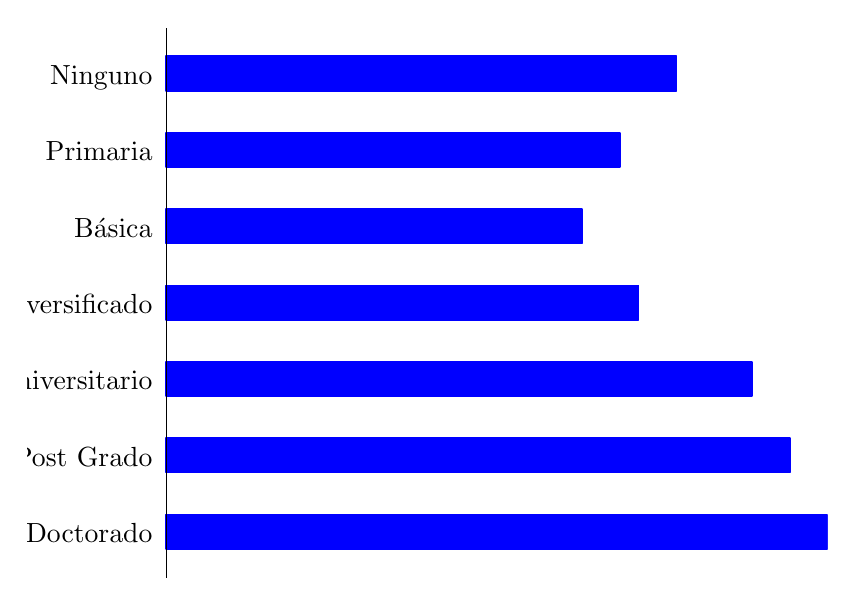
\begin{tikzpicture}[x=1pt,y=1pt]  % Created by tikzDevice version 0.10.1 on 2016-02-29 14:47:24
% !TEX encoding = UTF-8 Unicode
\definecolor{fillColor}{RGB}{255,255,255}
\path[use as bounding box,fill=fillColor,fill opacity=0.00] (0,0) rectangle (289.08,198.74);
\begin{scope}
\path[clip] (  0.00,  0.00) rectangle (289.08,198.74);

\path[] (  0.00,  0.00) rectangle (289.08,198.74);
\end{scope}
\begin{scope}
\path[clip] (  0.00,  0.00) rectangle (289.08,198.74);

\path[] ( 50.00,  0.00) rectangle (289.08,198.74);

\path[] ( 50.00, 16.56) --
	(289.08, 16.56);

\path[] ( 50.00, 44.16) --
	(289.08, 44.16);

\path[] ( 50.00, 71.77) --
	(289.08, 71.77);

\path[] ( 50.00, 99.37) --
	(289.08, 99.37);

\path[] ( 50.00,126.97) --
	(289.08,126.97);

\path[] ( 50.00,154.58) --
	(289.08,154.58);

\path[] ( 50.00,182.18) --
	(289.08,182.18);
\definecolor{drawColor}{RGB}{0,0,255}
\definecolor{fillColor}{RGB}{0,0,255}

\path[draw=drawColor,line width= 0.6pt,line join=round,fill=fillColor] ( 50.00, 10.35) rectangle (289.08, 22.77);

\path[draw=drawColor,line width= 0.6pt,line join=round,fill=fillColor] ( 50.00, 37.95) rectangle (275.42, 50.38);

\path[draw=drawColor,line width= 0.6pt,line join=round,fill=fillColor] ( 50.00, 65.56) rectangle (261.76, 77.98);

\path[draw=drawColor,line width= 0.6pt,line join=round,fill=fillColor] ( 50.00, 93.16) rectangle (220.77,105.58);

\path[draw=drawColor,line width= 0.6pt,line join=round,fill=fillColor] ( 50.00,120.76) rectangle (200.28,133.19);

\path[draw=drawColor,line width= 0.6pt,line join=round,fill=fillColor] ( 50.00,148.37) rectangle (213.94,160.79);

\path[draw=drawColor,line width= 0.6pt,line join=round,fill=fillColor] ( 50.00,175.97) rectangle (234.43,188.39);
\definecolor{drawColor}{RGB}{0,0,0}

\path[draw=drawColor,line width= 0.1pt,line join=round] ( 50.00,  0.00) -- ( 50.00,198.74);

\path[] ( 50.00,  0.00) rectangle (289.08,198.74);
\end{scope}
\begin{scope}
\path[clip] (  0.00,  0.00) rectangle (289.08,198.74);

\path[] ( 50.00,  0.00) --
	( 50.00,198.74);
\end{scope}
\begin{scope}
\path[clip] (  0.00,  0.00) rectangle (289.08,198.74);
\definecolor{drawColor}{RGB}{0,0,0}

\node[text=drawColor,anchor=base east,inner sep=0pt, outer sep=0pt, scale=  1.00] at ( 45.05, 12.65) {Doctorado};

\node[text=drawColor,anchor=base east,inner sep=0pt, outer sep=0pt, scale=  1.00] at ( 45.05, 40.26) {Post Grado};

\node[text=drawColor,anchor=base east,inner sep=0pt, outer sep=0pt, scale=  1.00] at ( 45.05, 67.86) {Universitario};

\node[text=drawColor,anchor=base east,inner sep=0pt, outer sep=0pt, scale=  1.00] at ( 45.05, 95.46) {Diversificado};

\node[text=drawColor,anchor=base east,inner sep=0pt, outer sep=0pt, scale=  1.00] at ( 45.05,123.07) {Básica};

\node[text=drawColor,anchor=base east,inner sep=0pt, outer sep=0pt, scale=  1.00] at ( 45.05,150.67) {Primaria};

\node[text=drawColor,anchor=base east,inner sep=0pt, outer sep=0pt, scale=  1.00] at ( 45.05,178.27) {Ninguno};
\end{scope}
\begin{scope}
\path[clip] (  0.00,  0.00) rectangle (289.08,198.74);

\path[] ( 47.25, 16.56) --
	( 50.00, 16.56);

\path[] ( 47.25, 44.16) --
	( 50.00, 44.16);

\path[] ( 47.25, 71.77) --
	( 50.00, 71.77);

\path[] ( 47.25, 99.37) --
	( 50.00, 99.37);

\path[] ( 47.25,126.97) --
	( 50.00,126.97);

\path[] ( 47.25,154.58) --
	( 50.00,154.58);

\path[] ( 47.25,182.18) --
	( 50.00,182.18);
\end{scope}
  \end{tikzpicture}}{Instituto Nacional de Estadística, con datos del Ministerio de Educación}

\cajota{Deserción en los departamentos}{El mapa muestra en color celeste los departamentos con las menores tasas de deserción en básicos, que en el 2013 fueron: Izabal 2.9\%, Guatemala 2.6\% y Quetzaltenango 1.3\%.
	
	 Los departamentos con las mayores tasas  de deserción en básico: Huehuetenango 7.0\%, El Progreso 6.9\% y Sololá 6.3\%.}{Tasa de deserción del ciclo de educación básica}{Por departamento, año 2014, en porcentaje}{\includegraphics[width=52\cuadri]{graficas/basicos/1_22.pdf}}{Instituto Nacional de Estadística, con datos del Ministerio de Educación}




\cajita{Aprobación}{La tasa de aprobación en básico se refiere a la cantidad de alumnos que culminaron y aprobaron el ciclo lectivo.
	
	En el año 2009 fue del 68.4\% y en el año 2014 fue de 71.6\%, que representó un aumento en 3.2 puntos porcentuales.}{Tasa de aprobación del ciclo de educación básica}{República de Guatemala, serie histórica, en porcentaje}{\ \\[0mm]\begin{tikzpicture}[x=1pt,y=1pt]  % Created by tikzDevice version 0.7.0 on 2015-08-28 13:10:46
% !TEX encoding = UTF-8 Unicode
\definecolor[named]{fillColor}{rgb}{1.00,1.00,1.00}
\path[use as bounding box,fill=fillColor,fill opacity=0.00] (0,0) rectangle (289.08,198.74);
\begin{scope}
\path[clip] (  0.00,  0.00) rectangle (289.08,198.74);
\definecolor[named]{drawColor}{rgb}{1.00,1.00,1.00}

\path[draw=drawColor,line width= 0.6pt,line join=round,line cap=round] (  0.00,  0.00) rectangle (289.08,198.74);
\end{scope}
\begin{scope}
\path[clip] (  0.00,  0.00) rectangle (289.08,198.74);

\path[] (  8.28, 17.78) rectangle (280.54,191.48);

\path[] (  8.28, 46.23) --
	(280.54, 46.23);

\path[] (  8.28, 87.36) --
	(280.54, 87.36);

\path[] (  8.28,128.48) --
	(280.54,128.48);

\path[] (  8.28,169.61) --
	(280.54,169.61);

\path[] (  8.28, 25.67) --
	(280.54, 25.67);

\path[] (  8.28, 66.80) --
	(280.54, 66.80);

\path[] (  8.28,107.92) --
	(280.54,107.92);

\path[] (  8.28,149.04) --
	(280.54,149.04);

\path[] (  8.28,190.17) --
	(280.54,190.17);

\path[] ( 39.69, 17.78) --
	( 39.69,191.48);

\path[] ( 92.05, 17.78) --
	( 92.05,191.48);

\path[] (144.41, 17.78) --
	(144.41,191.48);

\path[] (196.77, 17.78) --
	(196.77,191.48);

\path[] (249.13, 17.78) --
	(249.13,191.48);
\definecolor[named]{drawColor}{rgb}{0.00,0.00,1.00}

\path[draw=drawColor,line width= 1.7pt,line join=round] ( 39.69,163.85) --
	( 92.05,127.66) --
	(144.41,153.98) --
	(196.77,160.56) --
	(249.13,183.59);
\definecolor[named]{drawColor}{rgb}{0.00,0.00,0.00}

\node[text=drawColor,anchor=base,inner sep=0pt, outer sep=0pt, scale=  1.01] at ( 39.69,167.80) {68.4};

\node[text=drawColor,anchor=base,inner sep=0pt, outer sep=0pt, scale=  1.01] at ( 92.05,115.79) {66.2};

\node[text=drawColor,anchor=base east,inner sep=0pt, outer sep=0pt, scale=  1.01] at (141.30,153.98) {67.8};

\node[text=drawColor,anchor=base east,inner sep=0pt, outer sep=0pt, scale=  1.01] at (193.65,160.56) {68.2};

\node[text=drawColor,anchor=base,inner sep=0pt, outer sep=0pt, scale=  1.01] at (249.13,187.54) {69.6};
\definecolor[named]{fillColor}{rgb}{0.00,0.00,0.00}

\path[draw=drawColor,line width= 0.1pt,line join=round,fill=fillColor] (  8.28, 25.67) -- (280.54, 25.67);
\end{scope}
\begin{scope}
\path[clip] (  0.00,  0.00) rectangle (289.08,198.74);

\path[] (  8.28, 17.78) --
	(  8.28,191.48);
\end{scope}
\begin{scope}
\path[clip] (  0.00,  0.00) rectangle (289.08,198.74);
\definecolor[named]{drawColor}{rgb}{1.00,1.00,1.00}

\node[text=drawColor,text opacity=0.00,anchor=base east,inner sep=0pt, outer sep=0pt, scale=  1.00] at (  1.17, 21.76) {60.0};

\node[text=drawColor,text opacity=0.00,anchor=base east,inner sep=0pt, outer sep=0pt, scale=  1.00] at (  1.17, 62.89) {62.5};

\node[text=drawColor,text opacity=0.00,anchor=base east,inner sep=0pt, outer sep=0pt, scale=  1.00] at (  1.17,104.01) {65.0};

\node[text=drawColor,text opacity=0.00,anchor=base east,inner sep=0pt, outer sep=0pt, scale=  1.00] at (  1.17,145.13) {67.5};

\node[text=drawColor,text opacity=0.00,anchor=base east,inner sep=0pt, outer sep=0pt, scale=  1.00] at (  1.17,186.26) {70.0};
\end{scope}
\begin{scope}
\path[clip] (  0.00,  0.00) rectangle (289.08,198.74);

\path[] (  4.01, 25.67) --
	(  8.28, 25.67);

\path[] (  4.01, 66.80) --
	(  8.28, 66.80);

\path[] (  4.01,107.92) --
	(  8.28,107.92);

\path[] (  4.01,149.04) --
	(  8.28,149.04);

\path[] (  4.01,190.17) --
	(  8.28,190.17);
\end{scope}
\begin{scope}
\path[clip] (  0.00,  0.00) rectangle (289.08,198.74);

\path[] (  8.28, 17.78) --
	(280.54, 17.78);
\end{scope}
\begin{scope}
\path[clip] (  0.00,  0.00) rectangle (289.08,198.74);

\path[] ( 39.69, 13.51) --
	( 39.69, 17.78);

\path[] ( 92.05, 13.51) --
	( 92.05, 17.78);

\path[] (144.41, 13.51) --
	(144.41, 17.78);

\path[] (196.77, 13.51) --
	(196.77, 17.78);

\path[] (249.13, 13.51) --
	(249.13, 17.78);
\end{scope}
\begin{scope}
\path[clip] (  0.00,  0.00) rectangle (289.08,198.74);
\definecolor[named]{drawColor}{rgb}{0.00,0.00,0.00}

\node[text=drawColor,anchor=base,inner sep=0pt, outer sep=0pt, scale=  1.00] at ( 39.69,  2.85) {2009};

\node[text=drawColor,anchor=base,inner sep=0pt, outer sep=0pt, scale=  1.00] at ( 92.05,  2.85) {2010};

\node[text=drawColor,anchor=base,inner sep=0pt, outer sep=0pt, scale=  1.00] at (144.41,  2.85) {2011};

\node[text=drawColor,anchor=base,inner sep=0pt, outer sep=0pt, scale=  1.00] at (196.77,  2.85) {2012};

\node[text=drawColor,anchor=base,inner sep=0pt, outer sep=0pt, scale=  1.00] at (249.13,  2.85) {2014};
\end{scope}
  \end{tikzpicture}}{Instituto Nacional de Estadística, con datos del Ministerio de Educación}

\cajita{Aprobación por sexo}{La tasa de aprobación en básico por sexo, representó el 67.8\% para hombres y 75.7\% para las mujeres.}{Tasa de aprobación del ciclo de educación básica, por sexo}{República de Guatemala, año 2014, en porcentaje}{\ \\[0mm]\begin{tikzpicture}[x=1pt,y=1pt]  \input{graficas/basicos/1_24.tex}  \end{tikzpicture}}{Instituto Nacional de Estadística, con datos del Ministerio de Educación}

\cajota{Aprobación en los departamentos}{Los departamentos con las menores tasas de aprobación en básico en el 2014 fueron: Chimaltenango 68.1\%, Quetzaltenango 63.2\% y Sacatepéquez 61.1\%,
	
	 Los departamentos con las mayores tasas de aprobación en básico fueron: Petén 79.6\%, Chiquimula 78.3\% y Quiché 77.2\%. 
	 
	 El departamento de Guatemala presentó una tasa de aprobación de 70.6\%.}{Tasa de aprobación del ciclo de educación básica}{Por departamento, año 2014, en porcentaje}{\includegraphics[width=52\cuadri]{graficas/basicos/1_25.pdf}}{Instituto Nacional de Estadística, con datos del Ministerio de Educación}



